\documentclass[11pt,letterpaper]{article}
\usepackage[utf8]{inputenc}
\usepackage[english]{babel}
\usepackage{amsmath}
\usepackage{amsfonts}
\usepackage{amssymb}
\usepackage[left=1in,right=1in,top=1in,bottom=1in]{geometry}
\usepackage{fancyhdr}
\usepackage{tikz}
\usepackage{graphicx}
\usepackage{float}
\usepackage[style=numeric, sorting=none]{biblatex}
\usepackage{subfig}
\usepackage{subfloat}
\usepackage{verbatim}
\addbibresource{citation.bib}
\def\hpd{homeless population density}
\def\ct{census track}
\def\k{$\textbf{k}$}

\begin{document}

\begin{titlepage}
\begin{center}
\vspace*{6cm}

\huge\textbf{Homeless Population}\\[3mm]
\Large Ryan Du, Sanjay Shukla, Hannah Ross, Xiang Yang Ng\\[1mm]

Math 199, Spring 2018

Advisor: Michael Lindstrom
\vfill
Draft Known Issue:
\begin{itemize}
\item Ryan (Neural Network)
\begin{itemize}
    \item The text in typewriter font are comments
    \item Method section, some of the math are not perfectly concrete
    \item Citation is not complete and accurate.
\end{itemize}
\end{itemize}
\end{center}
\end{titlepage}

\tableofcontents 

\newpage

\section{Introduction}

Homelessness is a prevalent issue in the Los Angeles area, and it is an issue that touches many different people in society. Previous models of homeless migration have acknowledged how homeless people are portrayed as highly mobile, and yet the migration behavior has not been systematically analyzed. 

There are a variety of forces that move homeless individuals including planned physical and social change programs such as urban renewal, slum clearance, highway construction, ‘Greyhound therapy’, and police sweeps of encampments. In a study predicting the movement of homeless young adults, HYA’s were identified as a subset of the population that were most receptive to care provided by agencies. This motivates our systematic study of homelessness which can serve to better inform agency initiatives that serve the homeless young adult population \cite{doi:10.1086/696129}.


The homeless migrant population that we intend to analyze includes a variety of sub-populations, each with their own unique causes for homelessness and motivations for moving. Among these sub-populations are homeless young adults, of which 60 percent self-identify as travelers. In one investigation into the correlates of homelessness in adolescents, 37 percent of homeless young adults are reported to of left home due to parent disapproval, 33 percent due to parental sexual abuse, and 51 percent were thrown out by their parents. Over 47 percent of homeless adolescents report a history of sexual abuse with parents, and nearly 37 percent self-identify as LGBTQ in orientation \cite{litreview}.

These statistics remind us that the causes of homelessness can stretch beyond high costs of living or lack of employment. They serve as evidence that homelessness is the culmination of both economic and sociological circumstances.


Another significant sub-population of the greater Los Angeles homeless population are the homeless veterans of Los Angeles. In a study conducted by the American Journal of Public Health, it was discovered that homeless veterans and homeless non-veterans have very contrasting profiles. Veterans are more likely to be white, educated, to have a history of marriage, and were more likely to have alcohol issues rather than drug issues. In interviews conducted with 33 chronically and 26 acutely homeless veterans receiving transitional housing services in LA from 2003 to 2005, both groups had substantial physical, psychiatric, and social impairment. Their answers to interview questions revealed how health and substance abuse interacted with loss of support and eviction to exacerbate homelessness. In understanding this sub-group of the homeless population, it reminds us to consider alternative factors that need to be treated and addressed in order to treat the chronic issue of homelessness.


A study into the migration of veterans who received homeless services from the Department of Veterans Affairs analyzed the migration patterns for 113,000 homeless veterans who initiated use of the VA homeless services in 2011 or 2013. The study's model showed an estimated 0.9 percent gain in homeless veterans for every 10 degrees of average temperature gain \cite{VA}.Interestingly, in-migration tended to roughly balance out-migration in a region.

In understanding the fluctuations and patterns of homelessness, we will be in a better position to inform more impactful and efficient uses of resources that are being directed towards the homeless population.



\section{Data Management}
We used data from several sources: the Los Angeles Homeless Services Authority (LAHSA),
the housing and rental website Zillow, the public data platform DataLA, the Los Angeles County Metropolitan Transportation Authority, and the American Community Surveys.

We used LAHSA to obtain data about estimates of homeless populations by census track in the years 2017. 
Estimates describe counts of both unsheltered and sheltered homeless people, with additional data describing features of the homeless population itself, including the number of people in tents, cars, vans, and makeshift shelters. 

All data on census tract boundaries came from shapefiles on Los Angeles Geohub, a public platform for
geolocation data from Los Angeles County. The two main housing indices that we used were Zillow Rent Index (ZRI) and Zillow Home Value Index (ZHVI). The former tracks the median rent while the latter tracks the median home value within a certain area. We obtained both for all zip codes and then converted them to census tracts by locally averaging over zip codes.

We found information on features, i.e restaurants, overnight parking citations, crimes, total population for all census tracts through DataLA, an open data platform maintained by the city of Los Angeles. After obtaining street addresses for each of these features, we converted them into latitude/longitude points using Google Maps Geocoding API through Python scripting. Locations were converted from latitude/longitude points to California State Planar feet using MATLAB code "SP Proj" [11] that we obtained from Mathworks. Each state plane (x,y) coordinate, corresponding to a feature, was assigned to a census tract in MATLAB using Los Angeles shapefiles.

Locations of coffee shops were obtained by iteratively searching for coffee shops within a small radius using the Google Places API through Python scripting, which produced street addresses and latitude/longitude points, while latitude/longitude of homeless shelters and services were obtained from Los Angeles Geohub, whose data is maintained by the County of Los Angeles Location Management System. We then assigned these latitude/longitude points to census tracts using a similar process as above.

Finally, we obtained estimates of the median household incomes per census tract as of 2014, 2015, and 2016 from the
American Community Survey, a five-year estimate conducted by the United States Census Bureau. Geographic data was downloaded in geodatabase format and converted to a spreadsheet using the open source
geographic information systems software QGIS.

For information on grocery store locations, we used the address locations listed on YellowPages.com for all Ralphs and Trader Joes locations in the greater Los Angeles area. The street addresses from the site were web scraped using the open source SelectorGadget tool to extract CSS features from the web site, and using the rvest library in R Studio to integrate the information into data objects. The web-scraped street address locations were then converted into latitude and longitude geocode locations using the ggmap library in R studio, and the Google Maps Geocoding API.

The distances to the nearest Ralphs and nearest Trader Joes were calculated for each census tract by finding the store locations with the minimum haversine distance to the centroid of each census tract. This was computed using the haversine distance function from the geosphere library for R studio.

Similarly, the information for the proximity of each census tract to the nearest public library was obtained by using the latitude and longitude locations for all public library locations available on DataLA. Public library locations data were available on DataLA as a dataset with observations for each public library listed in Los Angeles. The street addresses of these public libraries were converted into latitude/longitude points with the Google Maps Geocoding API. We identified the minimum haversine distances from the centroid of each census tract to each public library location.

\section{Techniques and Models}

\subsection{Normalizing Data into Percentiles}
Los Angeles had certain features that exhibited huge disparities among census tracts such as Median Household Incomes and Zillow Home and Rent Index. In order to account for these large disparities, we normalized the data according to percentile ranks. First, suppose we have a data matrix, $\textbf{D}	\in\mathbb{R}^{nxm}$ where the rows represent the census tracts and the columns represents the features associated with the census tracks. Then, we rank all the elements in the column from 1 to the number of observations in the column. If some elements have the same value, then they have the average rank. Denote the census track i for feature j converted to its percentile rank be entries, $\textbf{R}^{ij}$, where $i\in\{1,2,...,n\}$ and $j\in\{1,2,...,m\}$. We'll divide all of the entries by the number of census tracks, such that the new normalized matrix be $\textbf{A}$, where for all i,j,
\begin{align}
  \textbf{A}_{ij}  = \frac{\textbf{R}^{ij}}{n}  
\end{align}\\

\subsection{Topic Modeling}
Using the data normalized into percentiles we are left with a ${\rm I\!R}^{nxm}$ data matrix denoted \textbf{A}. Let $\textbf{A}_{i.}$ corresponds to a row of a census tract and with the features within that census tract, $\textbf{A}_{.j}$ correspond to a column of only census tracts or only an individual feature, and $\textbf{A}_{ij}$ correspond to element $(i,j)$.

We used nonnegative matrix factorization (NMF) in order to reduce the dimensions of our data to a topic matrix, $\textbf{H}^{nxk}$  and a weight weight matrix, $\textbf{W}^{kxm} $ which would approximate to our data matrix such that  \textbf{k} is the number of topics, $\textbf{W, H} > \textbf{0}$  and $\textbf{A} \approx \textbf{WH}$.

 To obtain the matrices for \textbf{H} and \textbf{W}, we minimize the Frobenius Norm by minimizing the least-squares function \cite{NIPS2000_1861}:
\begin{align}
\Vert \textbf{A}_{.  j} - \textbf{WH}_{.j} \Vert ^{2}
\end{align}

By compressing our data into smaller matrices, \textbf{H} and \textbf{W}, we reduce the dimensions of the data and will help avoid over-fitting when making predictive inferences on the relations between topics and their associated weights . 

We varied the rank \textbf{k} from $k=2$ to $k = 8$  in order to test whether a different number of topics could yield weight and topic matrices that would better represent the data. For each non-negative matrix factorization with varying rank \textbf{k}, we selected the top 10 census tracts with the highest weights for each topic and the homeless population density and plotted the centroids over a map of Los Angeles in order to visualize the clusters of data.

Moreover, for all \textbf{k}, we also find the correlation between the weights of each topic and the homeless population density. This is because we want to analyse the relationship between the topic matrix and the homeless population density to see if we could identify dynamics in the homeless population that could be explained by the topics. Denote $\textbf{W}_{.i}$, where i is the $i^{th}$ column of \textbf{A} and $\textbf{HPD}$ be homeless population density vector for all of the census tracks. The correlation between the weights of each topic and the homeless population density,$\rho(\textbf{HPD}, \textbf{W}_{.i})$:
\begin{align}
\rho(\textbf{HPD}, \textbf{W}_{.i})= \frac{1}{N-1}\sum_{k=1}^{n}\left(\frac{\textbf{HPD}_{k}-\mu_{\textbf{HPD}}}{\sigma_{\textbf{HPD}}}\right)\left(\frac{\textbf{W}_{ki}-\mu_{\textbf{W}_{.i}}}{\sigma_{\textbf{W}_{.i}}}\right)
\end{align}
where $\mu_{\textbf{HPD}}$ is the mean of $\textbf{HPD}$, $\sigma_{\textbf{HPD}}$ is the standard deviation of $\textbf{HPD}$, $\mu_{\textbf{W}_{.i}}$ is the mean of $\textbf{W}_{.i}$, $\sigma_{\textbf{W}_{.i}}$ is the standard deviation of $\textbf{W}_{.i}$
\begin{flushleft}

\end{flushleft}
After finding the correlation, we take the 2 topics that have the highest positive and highest negative correlation respectively with the homeless population density. That's because the higher the absolute value of the correlation, the better the topics are at explaining the homeless population. First, convert the census tracks to its corresponding longitudes and latitudes. We then plot a heat map graph of weights for each topic and homeless population density on the longitude-latitude plane. 

We also find the local "variance" of the census track, by first normalizing the columns as z-scores. Then for each census tract with their corresponding features, $\textbf{A}_{i.}$, obtain the 5 "nearest" census tracks based on their "distance", i.e Frobenius norm of the pair of longitude and latitude of the census track and that of all the other census tracks. Denote $\textbf{A}_{k_{j}.}$ to be one of the "nearest" census tracks, where  $k_{j} \neq i$ and $j\in\{1,2,3,4,5\}$. Then we form a local data matrix with all the features within of the census tracks and its neighbours, i.e form a matrix $B^{i}\in \mathbb{R}^{jxm}$, such that 
\begin{align}B^{i} = \begin{pmatrix} -\textbf{A}_{i.}- \\
 -\textbf{A}_{k_{1}.}-\\ 
 -\textbf{A}_{k_{2}.}-\\
 -\textbf{A}_{k_{3}.}-\\
 -\textbf{A}_{k_{4}.}-\\
 -\textbf{A}_{k_{5}.}-\\
 \end{pmatrix}
\end{align}

At last, from (3), we take the sum of squares of all the elements of $B_{i}$, which we denote $SSB^{i}$:
\begin{align}
SSB^{i} = \sum_{j=1}^{5}\sum_{l=1}^{m}\Vert B^{i}_{jm} \Vert ^{2}
\end{align}
\subsection{Linear Models}

We created three linear models to predict the variation in three different categories of the homeless population. We divided the homeless population into three distinct categories: the shelter homeless population (totShelterPeople), the in-vehicle homeless population (totCarPeople, totVanPeople, and totCamperPeople), and the street homeless population (totTentPeople, totEncampPeople). We tried to explain variation in each category of the homeless population using the other homeless categories  and the collected features of each census tract including distance to the nearest Ralphs, distance to the nearest Trader Joes, distance to the nearest public library, the number of citations, the number of coffee shops, the number of restaurants, the number of shelters, the total number of cars, the 2015 ZRI, the 2016 ZRI, the 2017 ZRI, the 2015 ZHVI, the 2016 ZHVI, the 2017 ZHVI, the median home income, the number of affordable housing units,  the number of bus stops , the 2015 Housed Population, the total 2015 homeless population, the total 2016 homeless population, and census tract square millage. 

In the modeling process for each of these three homeless population categories, we controlled for issues of high multicolinearity by eliminating predictors that had variation inflation factors greater than 10, corresponding to redundant predictors whose variations are more than 90\% explained by the variation of the other predictors (5). This is in line with Hair et. al. (1995), which maintains that 10 is the maximum level of acceptable Variance Inflation Factor scores. In addition, we imposed transformations on the response variables in order to avoid violations of our models assumptions regarding constant variance and normality of the residuals.
\begin{align}
    &\mathrm {VIF_{i}} ={\frac {1}{1-R_{i}^{2}}}
\end{align}
    
   % \mathbb{R_{i}^{2}}

    where (6) is the variation of the ith predictor that is explained by the remaining n-1 predictors.


Next, we constructed models for the three homeless populations using a forward stepwise regression process. In each step, this stepwise regression process will consider a variable for addition from the set of explanatory variables based on some prespecified criterion. We constructed models using both Akaike Information Criterion (AIC) and then Bayesian Information Criterion (BIC) as criterions. These are criteria for model selection that measure the trade-off between model fit and complexity of the model.  Lower AIC or BIC values indicate a better fit. Both AIC and BIC reward goodness of fit, and have penalties for too many predictors. BIC’s penalty for adding predictors is greater than AIC’s penalty which leads to BIC’s tendency to produce underfitting models, and AIC’s tendency to produce overfitting models. Below, k is the number of predictors, and $\hat L$ is the maximum value of the likelihood function for the model.

\begin{align}
    &\mathrm {AIC} =2k-2\ln({\hat {L}})\\
    &\mathrm {BIC} ={\ln(n)k-2\ln({\hat {L}})}.\ 
\end{align}

The forward step process begins with no predictors, and then proceeds to add predictors that will create a model with the lowest AIC and BIC values. Predictors are added individually until adding predictors no longer improves the calculated AIC or BIC for the model.

\subsection{Neural Networks}

We used neural networks to analyze the complex relationship between the time-dynamic data and the change in homeless population. Neural networks is a method that gets it's inspiration from the neurons of the human brain. The basic structure of a neural network is represented by the figure below. 

\def\layersep{2.5cm}

\begin{figure}[H]
\centering
\begin{tikzpicture}[shorten >=1pt,->,draw=black!50, node distance=\layersep]
    \tikzstyle{every pin edge}=[<-,shorten <=1pt]
    \tikzstyle{neuron}=[circle,fill=black!25,minimum size=17pt,inner sep=0pt]
    \tikzstyle{input neuron}=[neuron, fill=green!50];
    \tikzstyle{output neuron}=[neuron, fill=red!50];
    \tikzstyle{hidden neuron}=[neuron, fill=blue!50];
    \tikzstyle{annot} = [text width=4em, text centered]

    % Draw the input layer nodes
    \foreach \name / \y in {1,...,4}
    % This is the same as writing \foreach \name / \y in {1/1,2/2,3/3,4/4}
        \node[input neuron, pin=left:Input \#\y] (I-\name) at (0,-\y) {};

    % Draw the hidden layer nodes
    \foreach \name / \y in {1,...,5}
        \path[yshift=0.5cm]
            node[hidden neuron] (H-\name) at (\layersep,-\y cm) {};

    % Draw the output layer node
    \node[output neuron,pin={[pin edge={->}]right:Output}, right of=H-3] (O) {};

    % Connect every node in the input layer with every node in the
    % hidden layer.
    \foreach \source in {1,...,4}
        \foreach \dest in {1,...,5}
            \path (I-\source) edge (H-\dest);

    % Connect every node in the hidden layer with the output layer
    \foreach \source in {1,...,5}
        \path (H-\source) edge (O);

    % Annotate the layers
    \node[annot,above of=H-1, node distance=1cm] (hl) {Hidden layer};
    \node[annot,left of=hl] {Input layer};
    \node[annot,right of=hl] {Output layer};
\end{tikzpicture}
\caption{Structure of neural network}
\end{figure}

Imagine we have a size $m$ data-set with $n$ features with entries $(x_i,y_i)$, where $x_i$ is the feature value of a record and $y_i$ is the correct output.

Let's first stipulate some notations: We will use $W_{jk}^l$ denote the entry at $(j,k)$ in the weight matrix that connects the $(l-1)^{\text{th}}$ layer to the $l^{\text{th}}$ layer. Similarly, we  use $b_j^l$ for the bias at the $j^{\text{th}}$ position in the $l^{\text{th}}$ layer; use $h^l$ for the activation function of the $l^{\text{th}}$ layer; use $a_j^l$ for the activation for the activation at the $j^{\text{th}}$ position in the $l^{\text{th}}$ layer. \texttt{More detailed graph and the notation should be reflected on graph}

With these notation, we have the equation of the relation of activation at the $j^{\text{th}}$ position in the $l^{\text{th}}$ layer to the $(l-1)^{\text{th}}$ layer:
\begin{align}
&z_j^l=W^l_{jk}a_k^{l-1}+b^l_j &a^l=h^l(z^l) \label{eq:1}
\end{align}

We can rewrite the above equation with vectored form:
\begin{align*}
&z^l=W^la^{l-1}+b^l &a^l=h^l(z^l)
\end{align*}

The activation functions used in out models are: relu, sigmoid, and softmax. The relu function output the original input if the input in positive, 0 if the input is negative:
\begin{align}
\left\{
	\begin{array}{ll}
	h(z)=z&{\rm if~} z\leq 0\\
	h(z)=0&{\rm if~} z<0.
	\end{array}
\right.
\end{align}

\begin{figure}[H]
\centering
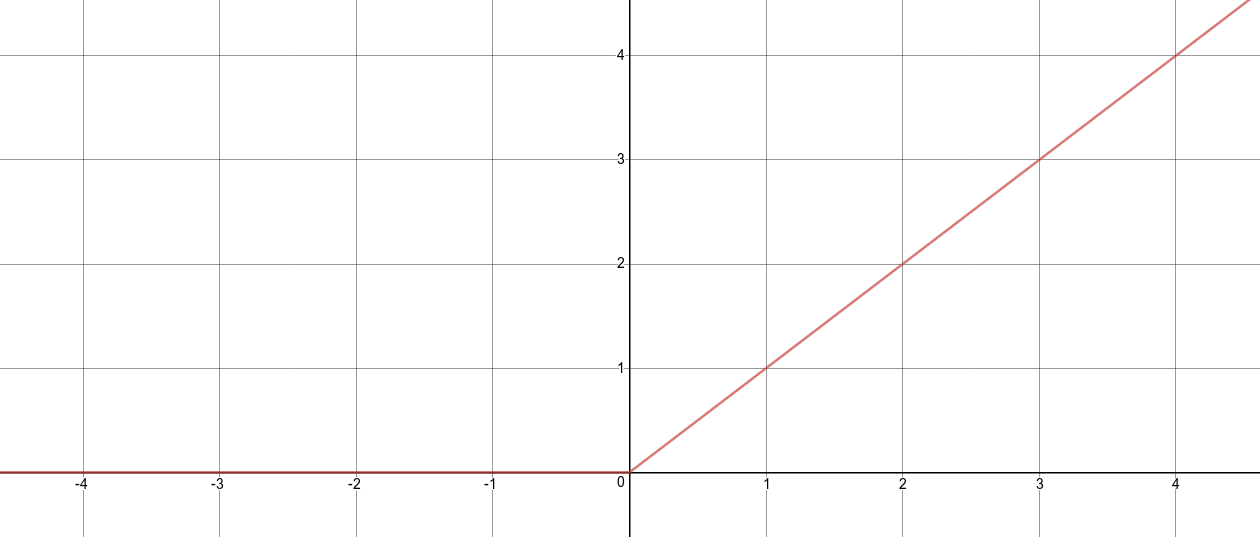
\includegraphics[scale=.15]{relu.png}
\caption{This figure shows the shape of the relu function.}
\end{figure}

The sigmoid function always output a number between -1 and 1. If has a steeper rate of increase when the input is near 0:
\begin{align}
h(x)=\frac{1}{1+e^{-x}}
\end{align}

\begin{figure}[H]
\centering
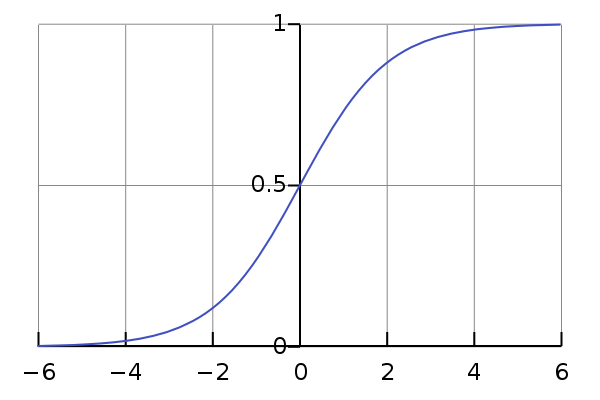
\includegraphics[scale=.3]{Logistic-curve.png}
\caption{This figure shows the shape of the sigmoid function.}
\end{figure}

The softmax function is a generalization of the logistic function that "squashes" a vector of arbitrary real values to a vector of real values, where each entry is in the range (0, 1), and all the entries adds up to 1:
$$h(z_j)={\frac {e^{z_{j}}}{\sum _{k=1}^{K}e^{z_{k}}}}$$

The algorithm learns how to best fit the data-set by trying to minimize a cost function. In our model, we used the cross-entropy cost function: \texttt{math needs more accurate}
\begin{align}
C = - \frac{1}{N}\sum_i^N\sum_{j} y_{ij} \log (a^L_{ij})\label{eq:2}
\end{align}

The method we used to minimize the cost is gradient descent. All weights and biases are updated against the direction of the cost function gradient for the values at that iteration. The learning
rate $\alpha$ is the size of step each iteration takes. For example, from the $i^{th}$ iteration to the $(i+1)^{th}$ iteration, the weight and bias should be updated by:
\begin{align}
&W^l_{i+1}=W_i^l-\alpha\frac{\partial C}{\partial W^l_{i}} &b^l_{i+1}=b_i^l-\alpha\frac{\partial C}{\partial b^l_{i}}
\end{align}

Adam is a variation of gradient descent. Adam calculates estimates of the mean and variance of the gradient and uses the ratio of the two to adjust the effective learning rate $\alpha$ for each parameter\cite{adam}.

In order to actually compute the gradient of the cost function against each elements of the weight and bias in each layer, we apply the chain rule repeatedly. This way of finding the gradient is called backpropagation\cite{NNDL}. The chain rule can be written out as this:
\begin{align}
&\frac{\partial C}{\partial b_k^l} = \frac{\partial C}{\partial a^L}\frac{\partial a^L}{\partial a^{L-1}}\frac{\partial a^{L-1}}{\partial a^{L-2}}\cdots \frac{\partial a^{l+1}}{\partial a^{l}}\cdot \frac{\partial a^{l}}{\partial b_k^l} \label{eq:3}\\
&\frac{\partial C}{\partial W_{pq}^l} = \frac{\partial C}{\partial a^L}\frac{\partial a^L}{\partial a^{L-1}}\frac{\partial a^{L-1}}{\partial a^{L-2}}\cdots \frac{\partial a^{l+1}}{\partial a^{l}}\cdot \frac{\partial a^{l}}{\partial W_{pq}^l} \label{eq:4}
\end{align}

We thus need to derive each term in the previous formula.

To make writing these formulas easier, we will be using the Einstein Summation notation where repeated indices are implicitly summed over. For example:
$$a_{ik}a_{ij}\equiv \sum_ia_{ik}a_{ij}$$

We will also be using the the Kronecker Delta, i.e:
$$\delta_{ij}=
	\left\{
		\begin{array}{ll}
		1&{\rm when~} i=j\\
		0&{\rm when~} i\neq j.
		\end{array}
	\right.
$$

From the equation of the cost function \ref{eq:2}, we can see that: \texttt{Work out math}
\begin{align}
\frac{\partial C}{\partial a^L_{ij}}&=\frac{-1}{N}\frac{y_{ij}}{a_{ij}} \label{eq:5}
\end{align}

The activation function for the $l^{\text{th}}$ layer $h^l$ is a function from $z^l$ to $a^l$, therefore:
\begin{align}
&\frac{\partial a_i^l}{\partial z_j^l} = \frac{\partial h_i^l(z_j^l)}{z_j^l} = \mathsf{J^l_{ij}}\nonumber\\
&\frac{\partial a^l}{\partial z^l} = \mathsf{J^l} \text{\ \ \ \ \ (the Jacobian matrix)} \label{eq:6}
\end{align}

From equation \ref{eq:1}, it is obvious that:
\begin{align}
\frac{\partial z_j^L}{\partial b_k^L}=\delta_{jk} \label{eq:7}
\end{align}

Also from equation \ref{eq:1}, we can see that:
\begin{align}
\frac{\partial z_j^l}{\partial W_{pq}^l}&=\frac{\partial}{\partial W_{pq}^l}(W^l_{jk}a_k^{l-1}+b_j^l)\nonumber\\
&= \delta_{jp}\delta_{kq}a_k^{l-1} = \delta_{jp}a_q^{l-1} \label{eq:8}
\end{align}

We can thus derive the function for the gradient: $\frac{\partial a_i^l}{\partial b_k^l}$ and $\frac{\partial a_i^l}{\partial W_{pq}^l}$\\
From \ref{eq:6} and \ref{eq:7}:
\begin{align}
\frac{\partial a_i^l}{\partial b_k^l} = \left(\frac{\partial a_i^l}{\partial z_j^l}\right)\delta_{kj} = \frac{\partial a_i^l}{\partial z_k^l} \label{eq:9}
\end{align}
From \ref{eq:6} and \ref{eq:8}:
\begin{align}
\frac{\partial a_i^l}{\partial W_{pq}^l}=\left(\frac{\partial a_i^l}{\partial z_j^l}\right)\delta_{jp}a_q^{l-1}=\left(\frac{\partial a_i^l}{\partial z_p^l}\right)a_q^{l-1} \label{eq:10}
\end{align}

To derive the expression for $\displaystyle \frac{\partial a^l}{\partial a^{l-1}}$, we have:
\begin{align}
\frac{\partial a_i^l}{\partial a_k^{l-1}}=\frac{\partial a_i^l}{\partial z_j^{l}}\frac{\partial z_j^l}{\partial a_k^{l-1}} \label{eq:11}
\end{align}
According to \ref{eq:1}:
\begin{align}
\frac{\partial z_j^l}{\partial a_k^{l-1}}=W_{jk}^l \label{eq:12}
\end{align}
Therefore we can use \ref{eq:6}, \ref{eq:12} and \ref{eq:11} to calculate:
\begin{align}
\frac{\partial a_i^l}{\partial a_k^{l-1}} = \mathsf{J^l_{ij}}W_{jk}^l \label{eq:13}
\end{align}
Now we have all the elements to calculate \ref{eq:3} and \ref{eq:4}

For neural network, it is also good practice to normalize the input data so that the data is on the same scale. There are two method that we used: Z-score and Principle Component Analysis (PCA). The data matrix $X$ is of dimension $\mathbb{R}^{m\times n}$, each row is a data point ($m$ of them) and each point has $n$ features.\\
Z-score normalization makes each feature (the column of our matrix) has 0 mean and 1 standard deviation. We first calculate the mean of of each column:
\begin{align}
M_j = \frac{\sum_i X_{ij}}{m}
\end{align}
Then we can calculate the standard deviation of the column:
\begin{align}
S_j = \sqrt{\frac{\sum_i {(X_{ij}-M_j)^2}}{m-1}}
\end{align}
The Z-score of the data in a column would be:
\begin{align}
Z_{ij}=\frac{X_{ij}-M_j}{S_j}
\end{align}
We do this calculation for each number in our matrix X, we can get the Z-score normalized data matrix Z, where the data in each column has a mean of 0 and the standard deviation of 1.

Principal component analysis (PCA) is a procedure that uses an orthogonal transformation to convert matrix variables into a set of linearly independent vectors called principal components. This transformation is defined in such a way that the first principal component has the largest possible variance (i.e.: accounts for as much of the variability in the data as possible), and each succeeding component in turn has the highest variance possible under the constraint that it is orthogonal to the preceding components. The resulting vectors are an orthogonal basis. PCA is sensitive to the relative scaling of the original variables, therefore we use the normalized $Z$ matrix derived above\cite{PCA}.

We use $T$ to denote the full principal components decomposition matrix of $Z$. It is common nowadays to use single value decomposition (SVD) to derive the matrix $T$.
\begin{align}
&Z = U\Sigma W^T\\
&T = ZW
\end{align}
And each column of $T$ is the principle component of $Z$, and column with smaller index explain more variance in the data. \texttt{More detailed math? Like about why they have the largest variance}

There are 818 census tracks that all the data we desire to use are reliable. The features we used are in two groups:
\begin{itemize}
\item Static: Citations, Coffee, Restaurants,Shelters, Crime Count, Bus Stops, Tract size in Square Miles;
\item Time Dynamic: Available Housing Units, Total Housing Units, Total Vacant Units, Unemployment Rate, Below Poverty Rate, Medium Rent As Percent Of Gross Income, Total Population, Medium Household Income, Medium Rent, Medium Value, Medium Monthly Housing Costs, ZRI, ZHVI.
\end{itemize}
For data in the static group, we took the value of 2016 and assumed that there is not much yearly changes. For data in the time dynamic group, we have data from 2014, 2015, and 2016.

We tried a ternary classification for the change of numbers of homeless populations in a census track. We implemented the neural networks in Tensorflow, a popular machine learning system\cite{Tensorflow}.

First, we divide the change in homeless population into three buckets. Roughly, the lower bucket represent a significant decrease in homeless population, the middle bucket represent a small, insignificant variation in the homeless population, and the higher bucket represent a significant increase in homeless population.

We used static data and time dynamic data (single year and change between years), to try to classify the change in homeless population. More specifically, for the time dynamic data, we used the change from 2014 to 2015 and the data of 2015 to classify the change in homeless population from 2015 to 2016; and the change from 2015 to 2016 and the data of 2016 to classify the change in homeless population from 2016 to 2017. We used the change of features of previous years to predict the change in homeless population because (1) ACS did not release the data for 2017 yet, and (2) the homeless population data is gathered during January, changes in previous years are reflected in changed in the year later \texttt{[cite data source]}. We compiled the data of changes in two years together and split them up with a ratio and 70\% and 30\%, 70\% of the data is used as the training set and 30\% of the data is used as the testing set.

We tried different method of preprocessing the data:
\begin{itemize}
\item Normalization
\item Principal Component Analysis (PCA)
\end{itemize}
We tried different cut off point for the buckets.\\
We tested different neural net work structure. We did trials on:
\begin{itemize}
\item Number of layers
\item Number of neurons in each layer
\item Activation function
	\begin{itemize}
	\item Relu
	\item Sigmoid
	\item Softmax
	\end{itemize}
\item Learning rate
\item Optimizer
	\begin{itemize}
	\item stochastic gradient descent
	\item Adam
	\end{itemize}
\end{itemize}

\section{Results}

\subsection{Topic Modeling}
By matching the top ten census tracts with correlating topics to homeless density with the centroid latitude and longitude coordinate, we were able to plot the geospatial locations of the census tracts with for a given topic. For each varying \textbf{k} the maps are as followed:

\begin{subfigures}
\begin{figure}[H]\centering
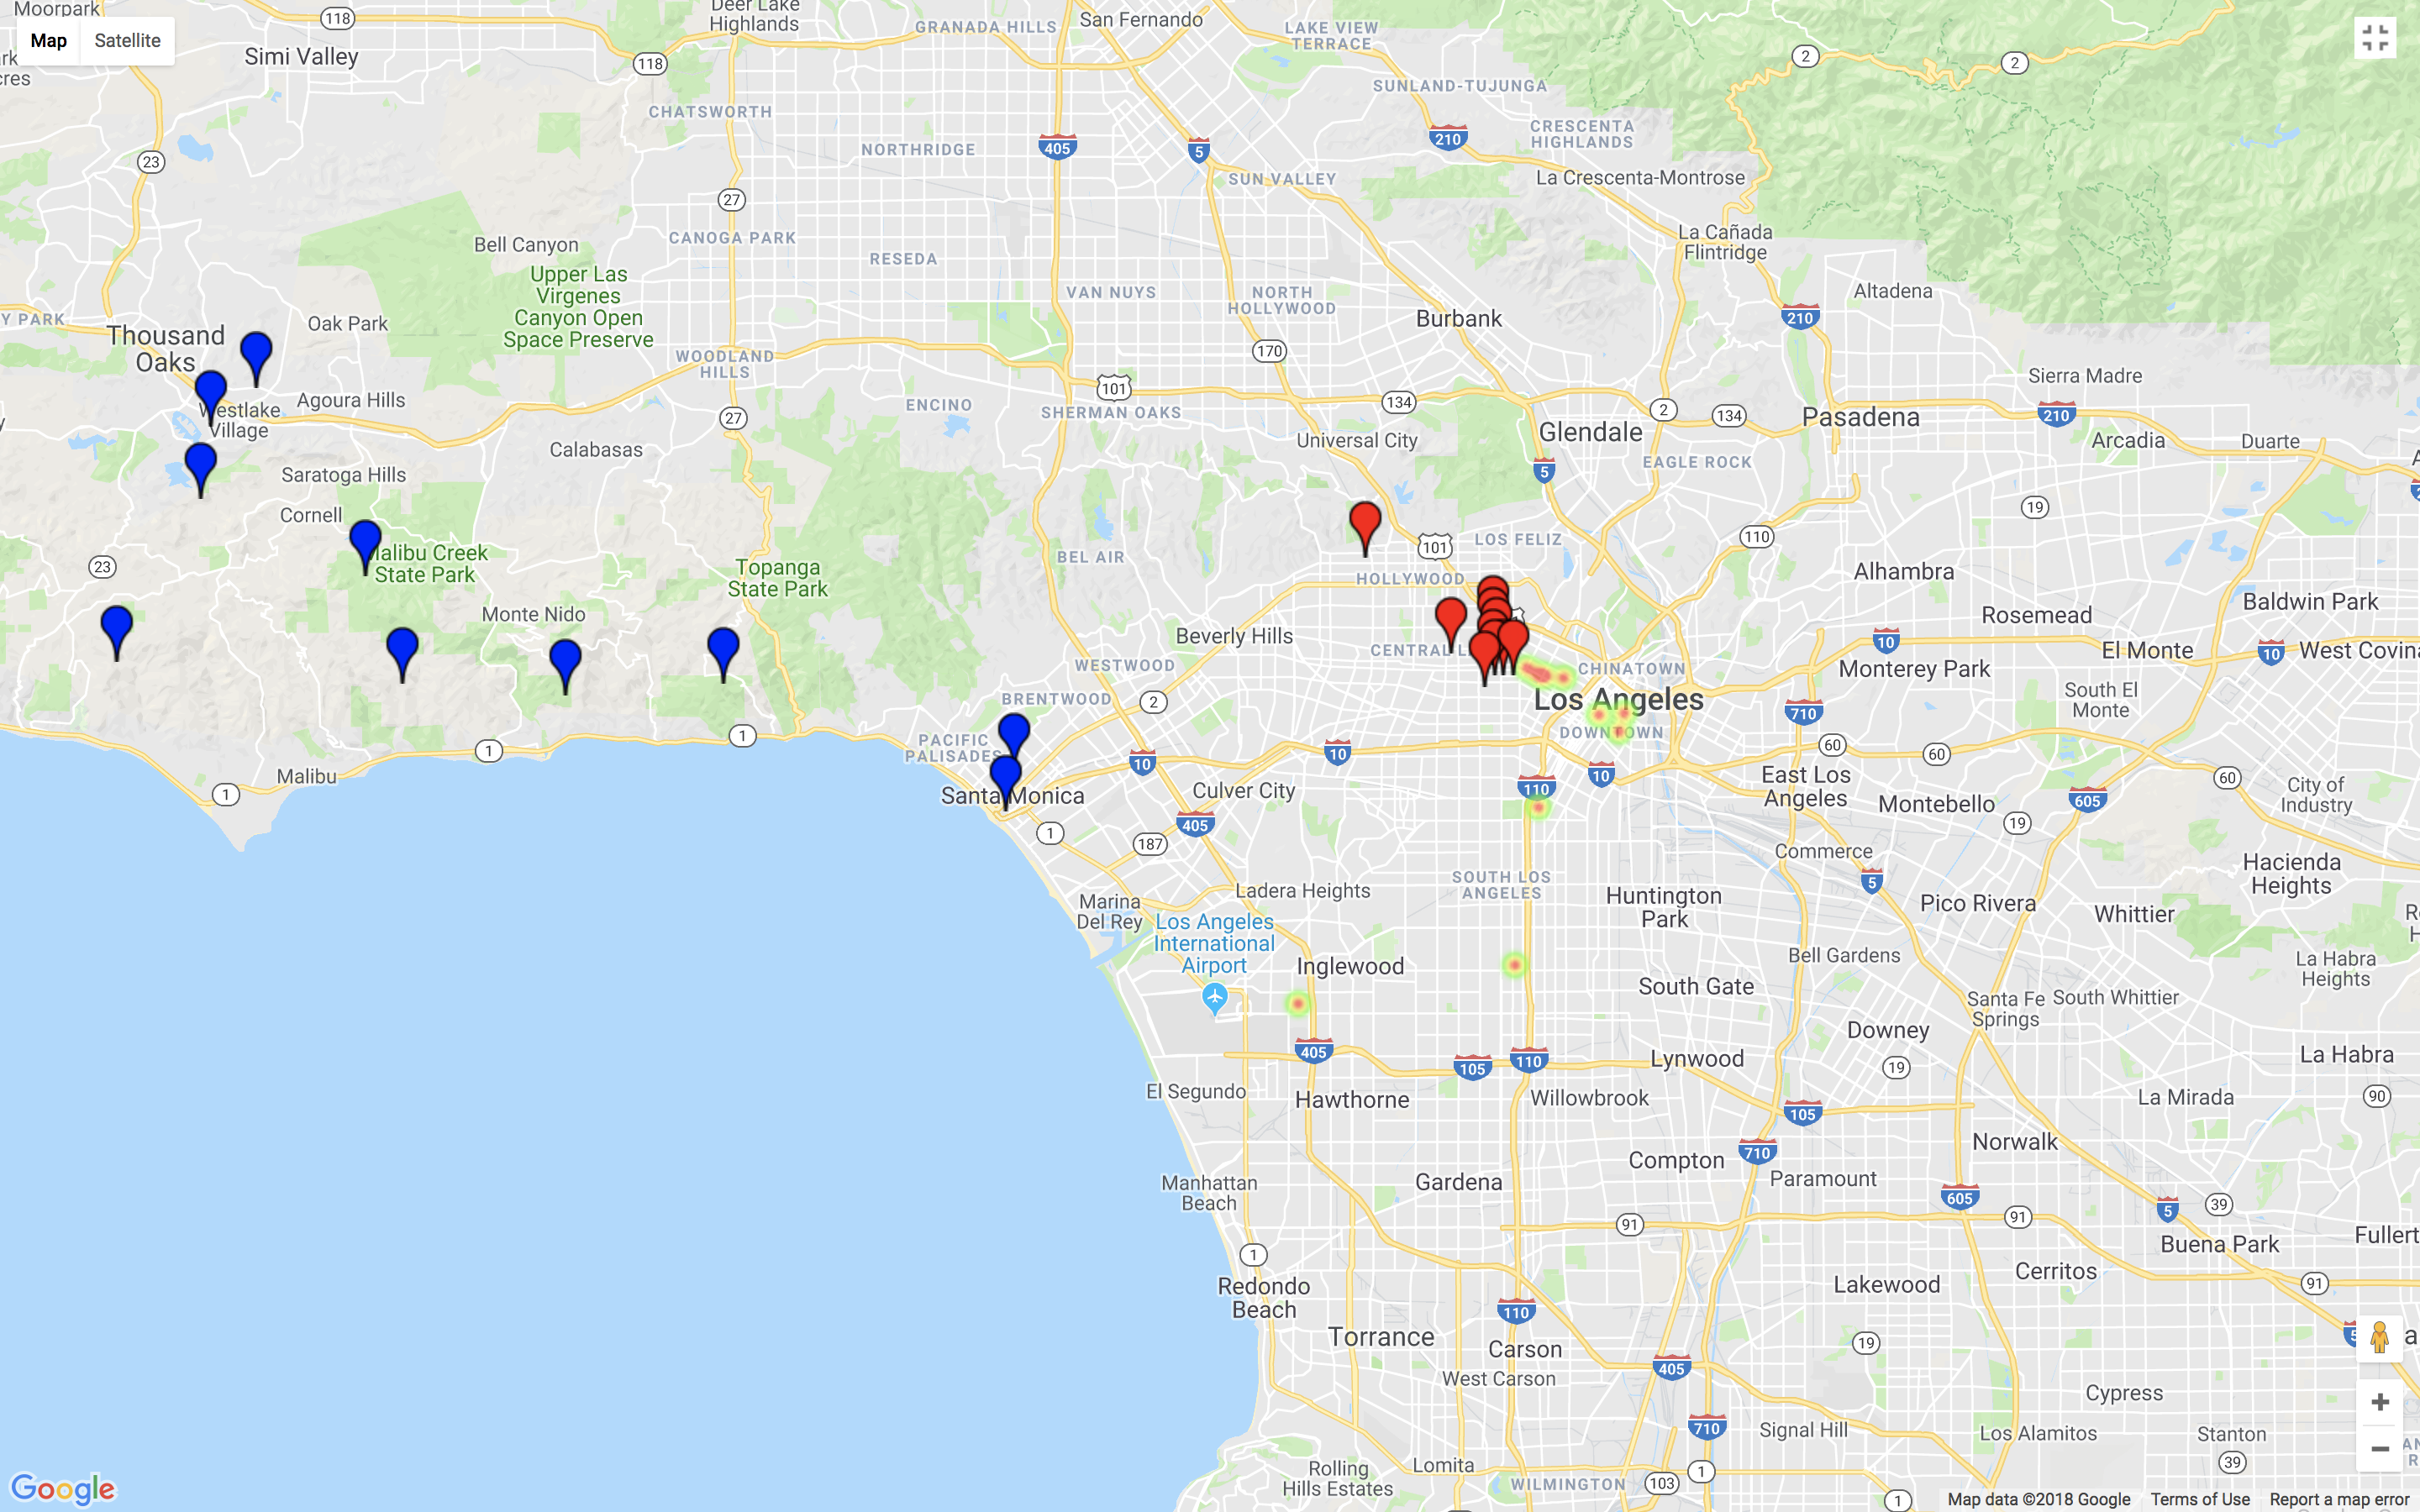
\includegraphics[width=\linewidth, height=0.4\textheight]{k=2.png}
\caption{$k=2$}
\end{figure}
%
\begin{figure}[H]\centering
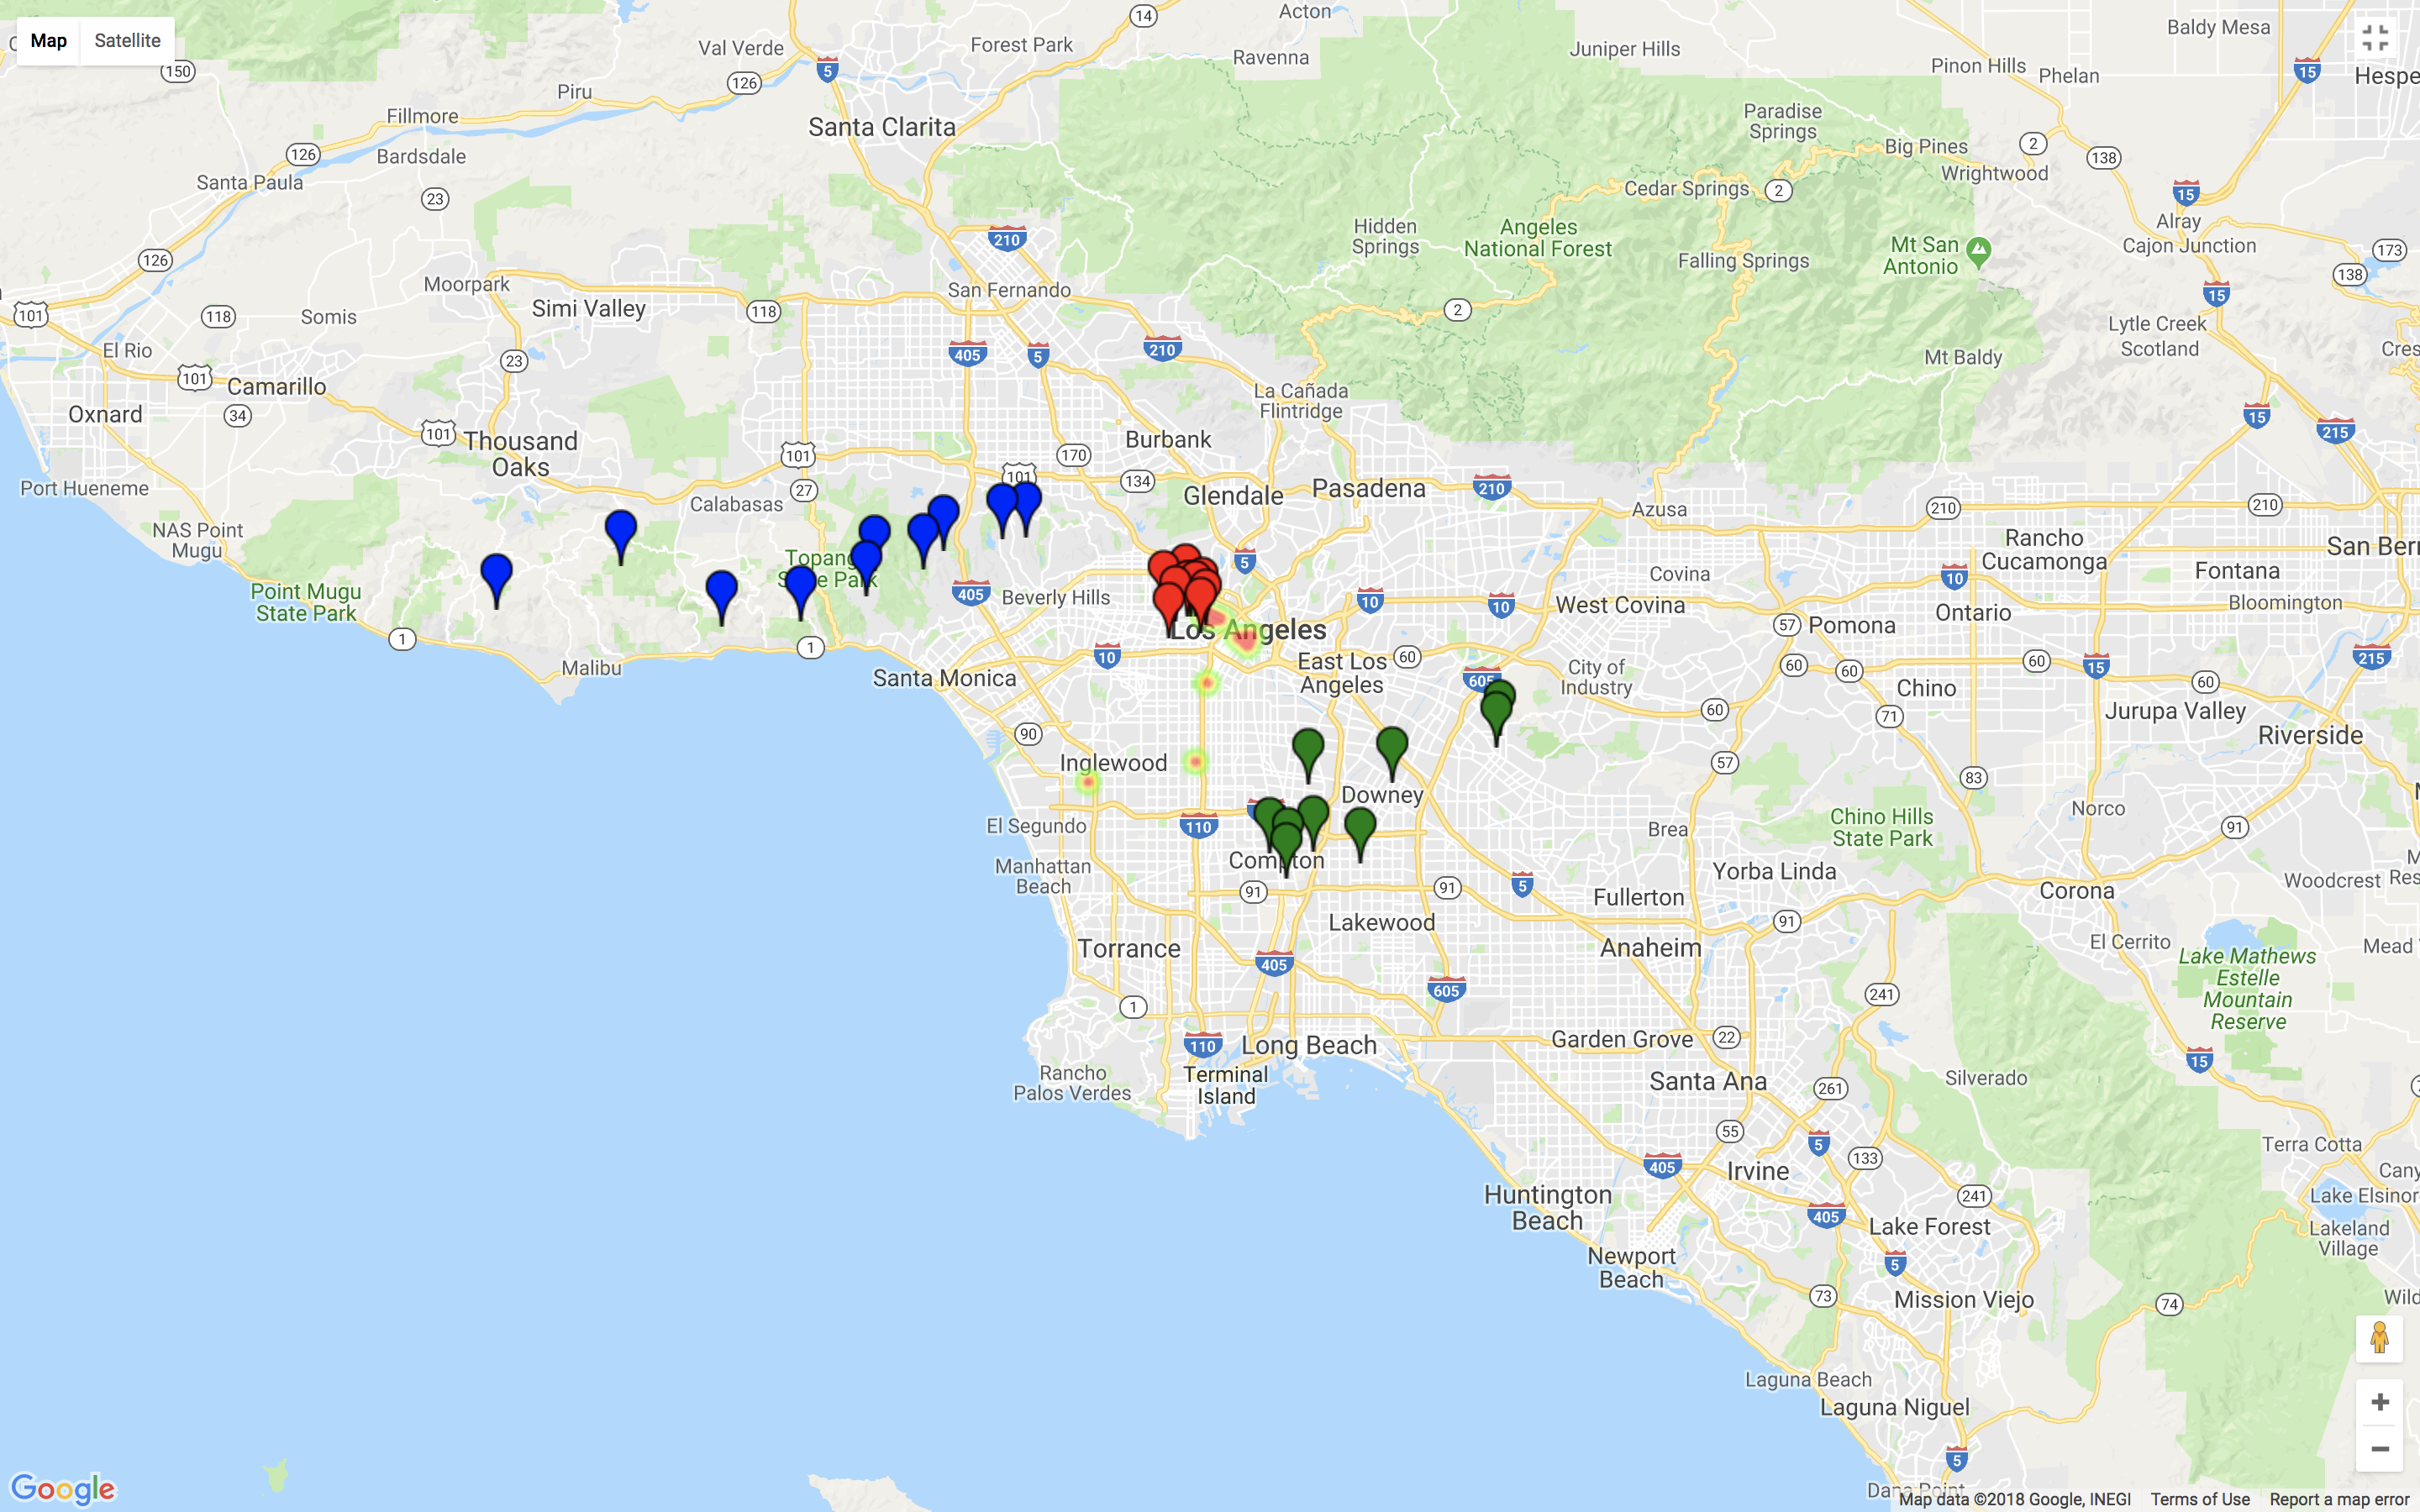
\includegraphics[width=\linewidth, height=0.4\textheight]{k=3.png}
\caption{$k=3$}
\end{figure}
%
\begin{figure}[H]\centering
  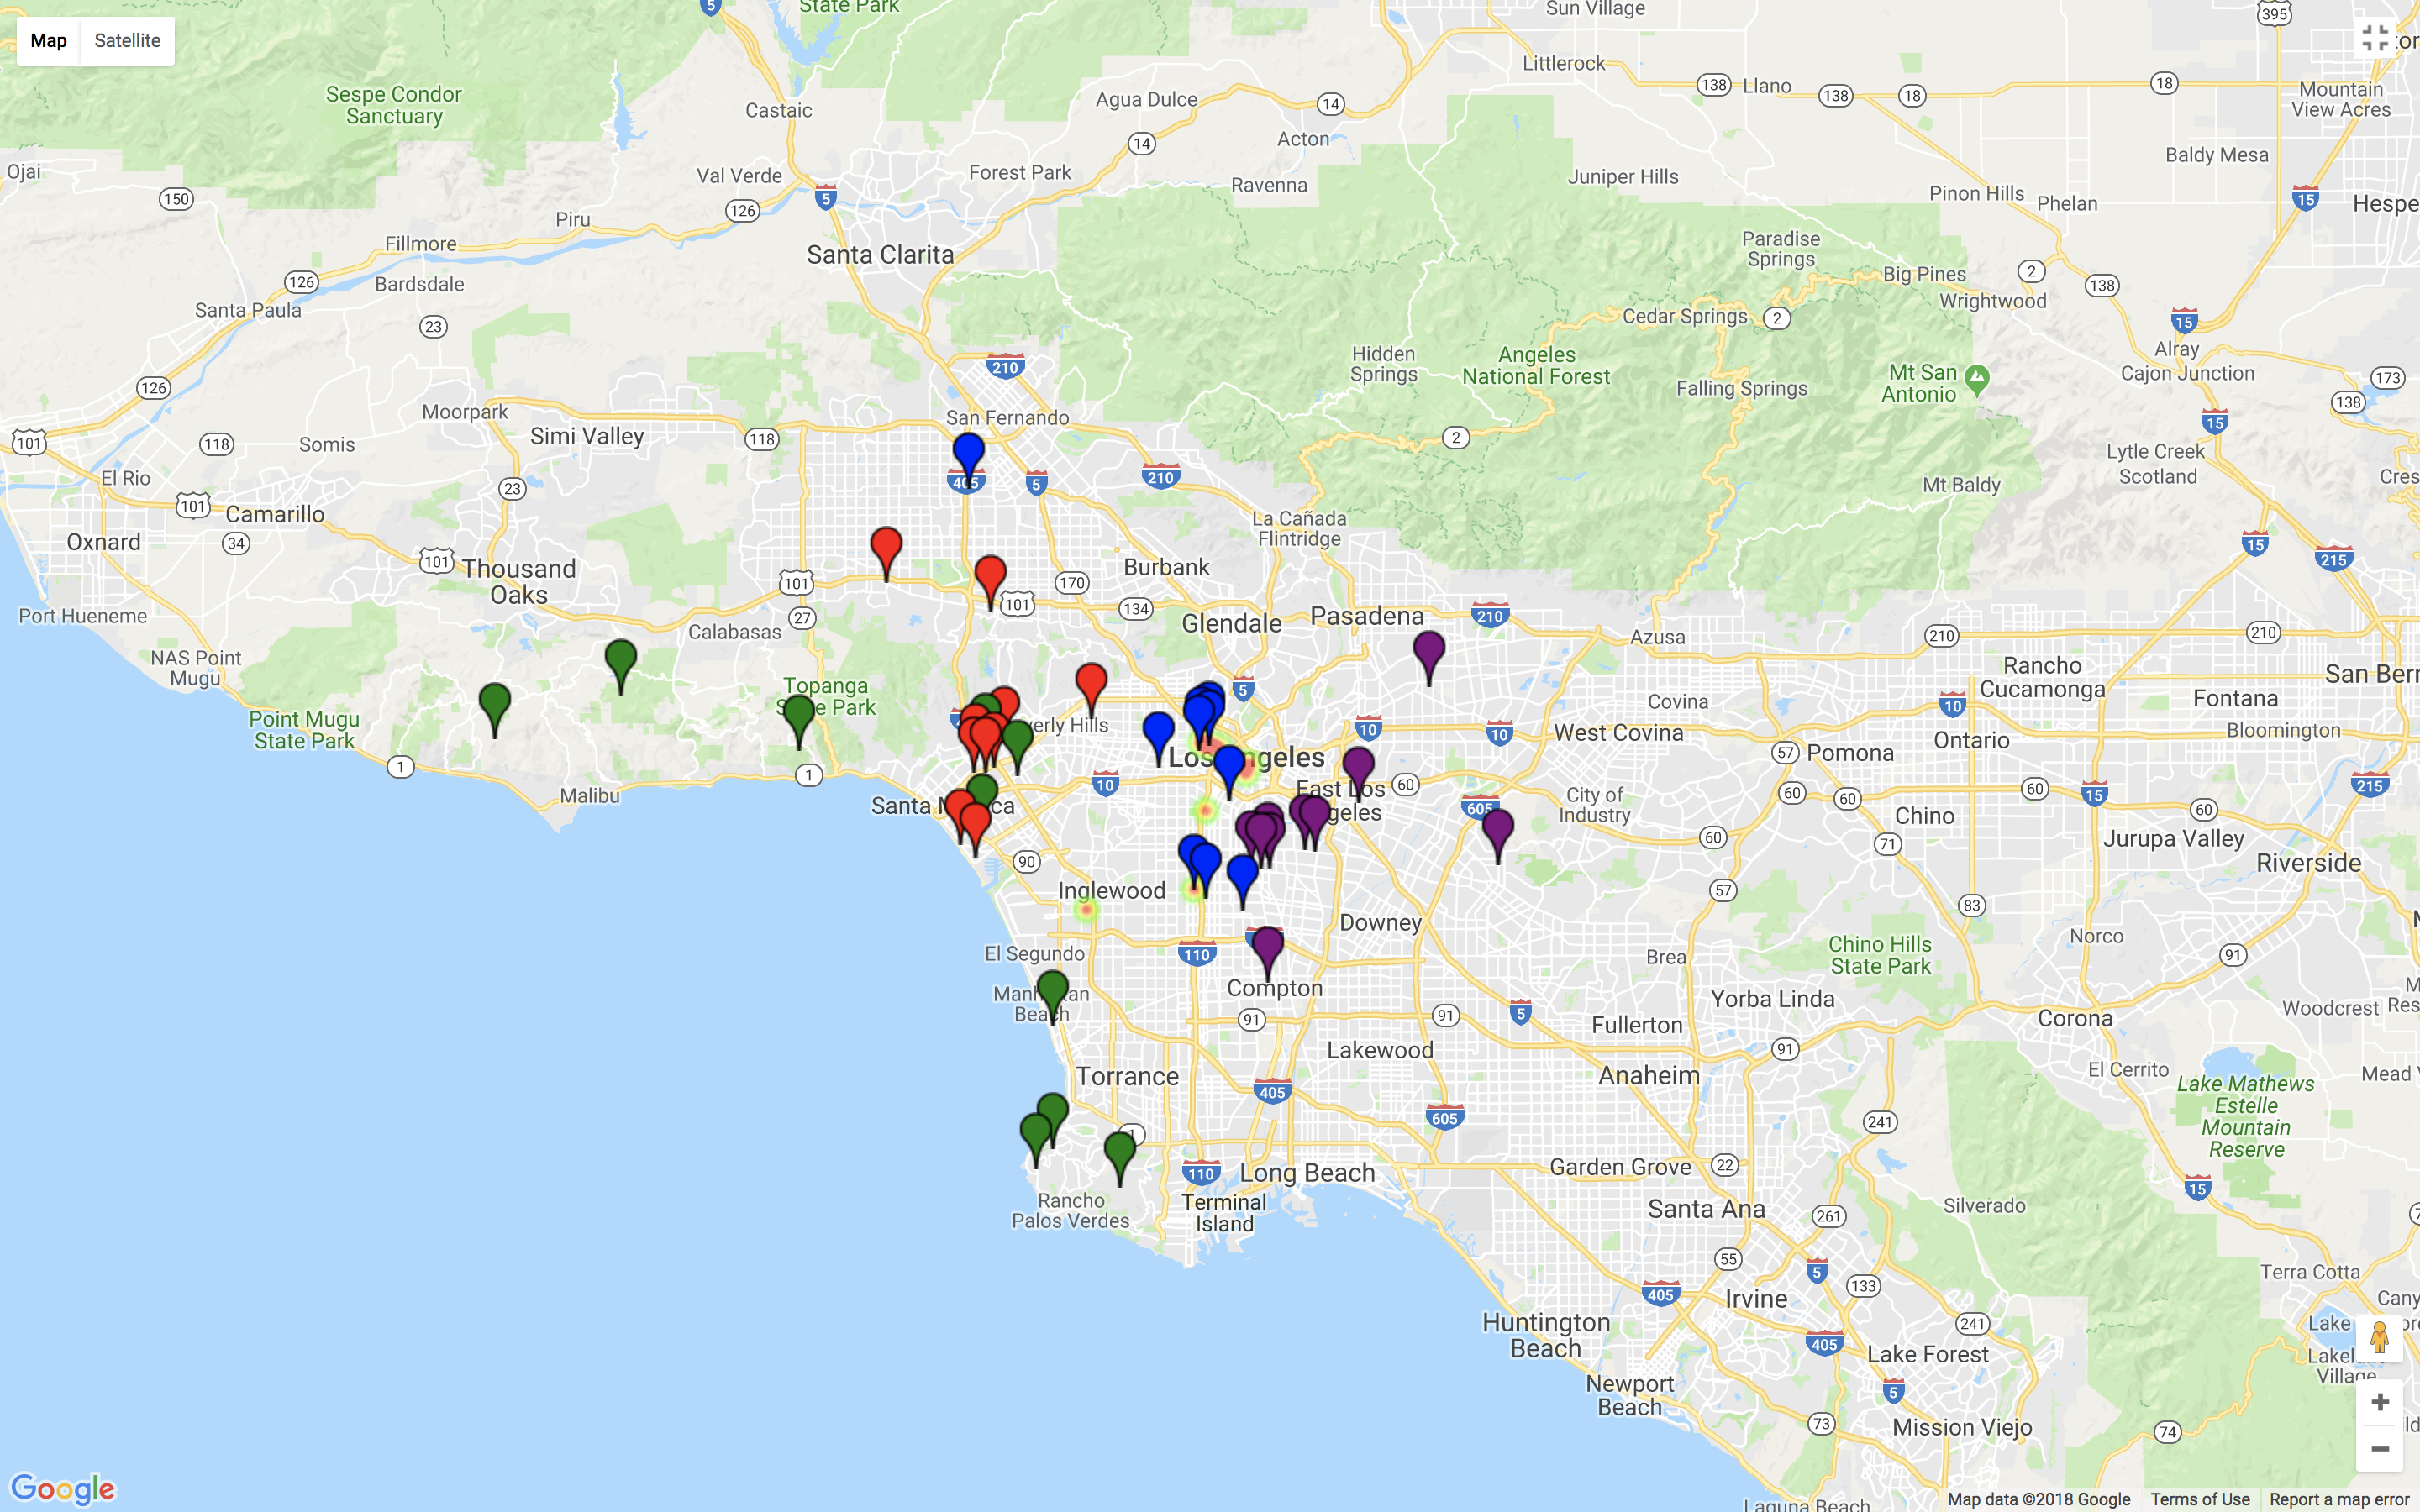
\includegraphics[width=\linewidth, height=0.4\textheight]{k=4.png}
  \caption{$k=4$}
\end{figure}
%
\begin{figure}[H]\centering
  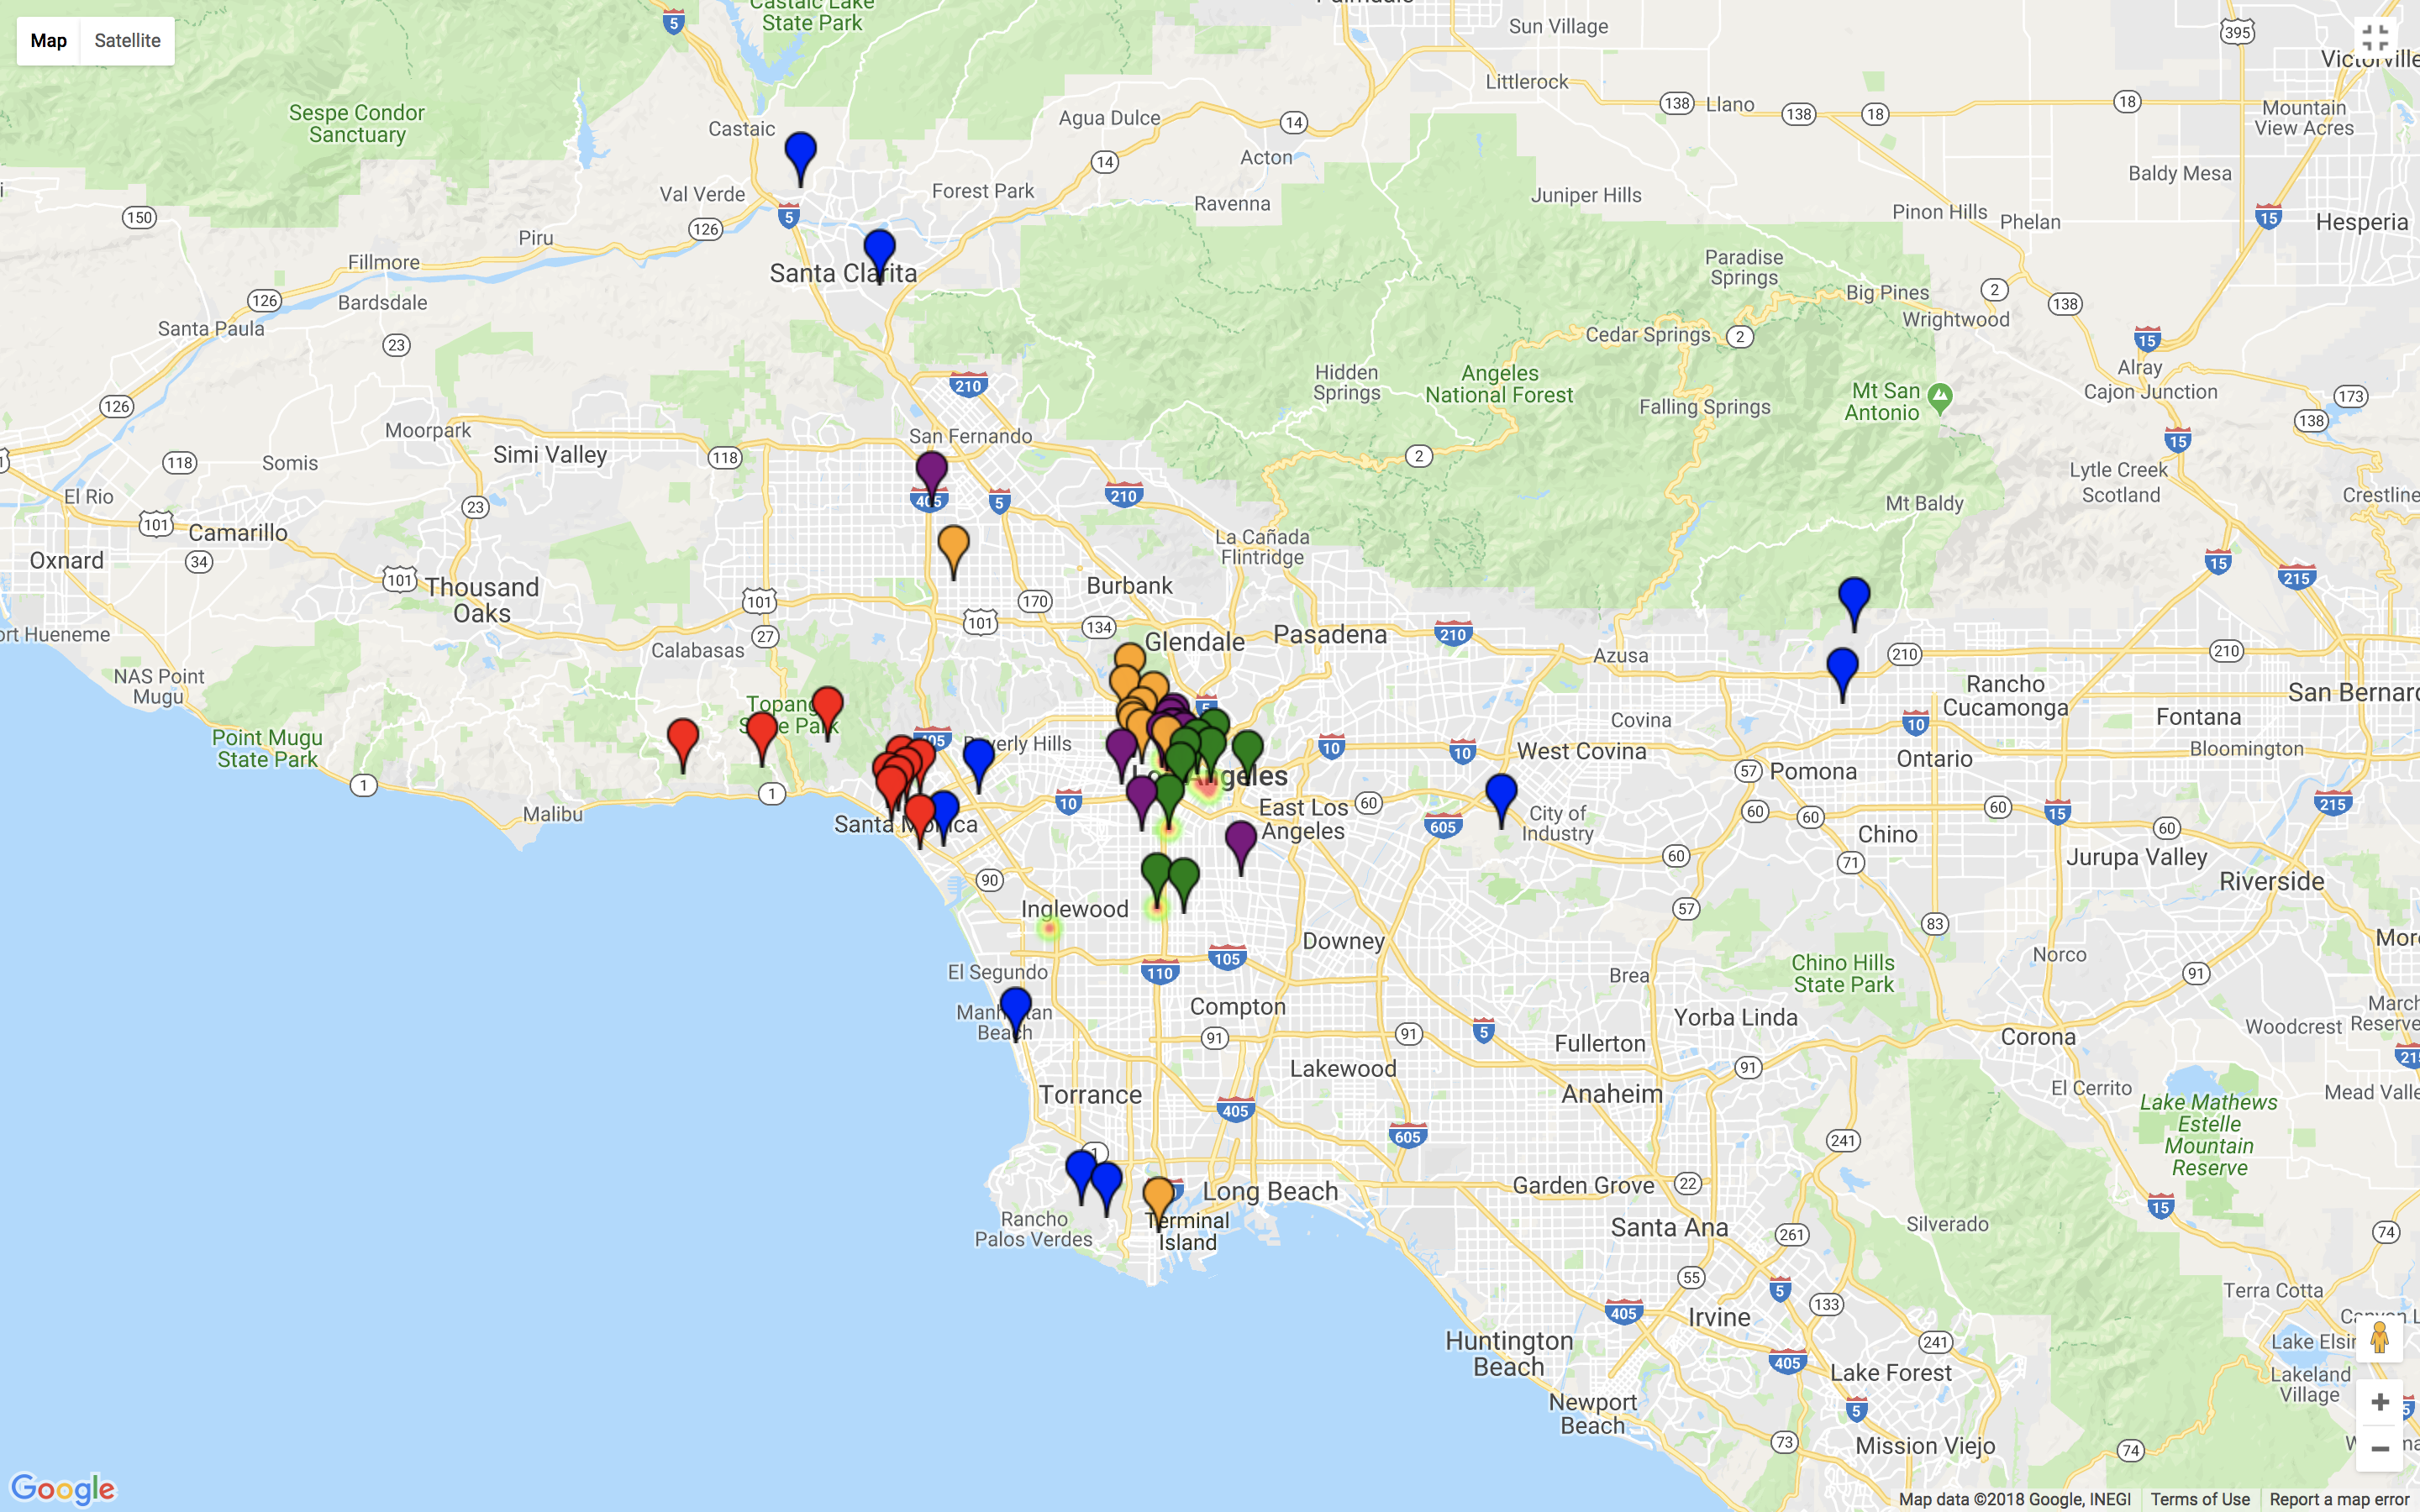
\includegraphics[width=\linewidth, height=0.4\textheight]{k=5.png}
  \caption{$k=5$}
\end{figure}

\begin{figure}[H]\centering
  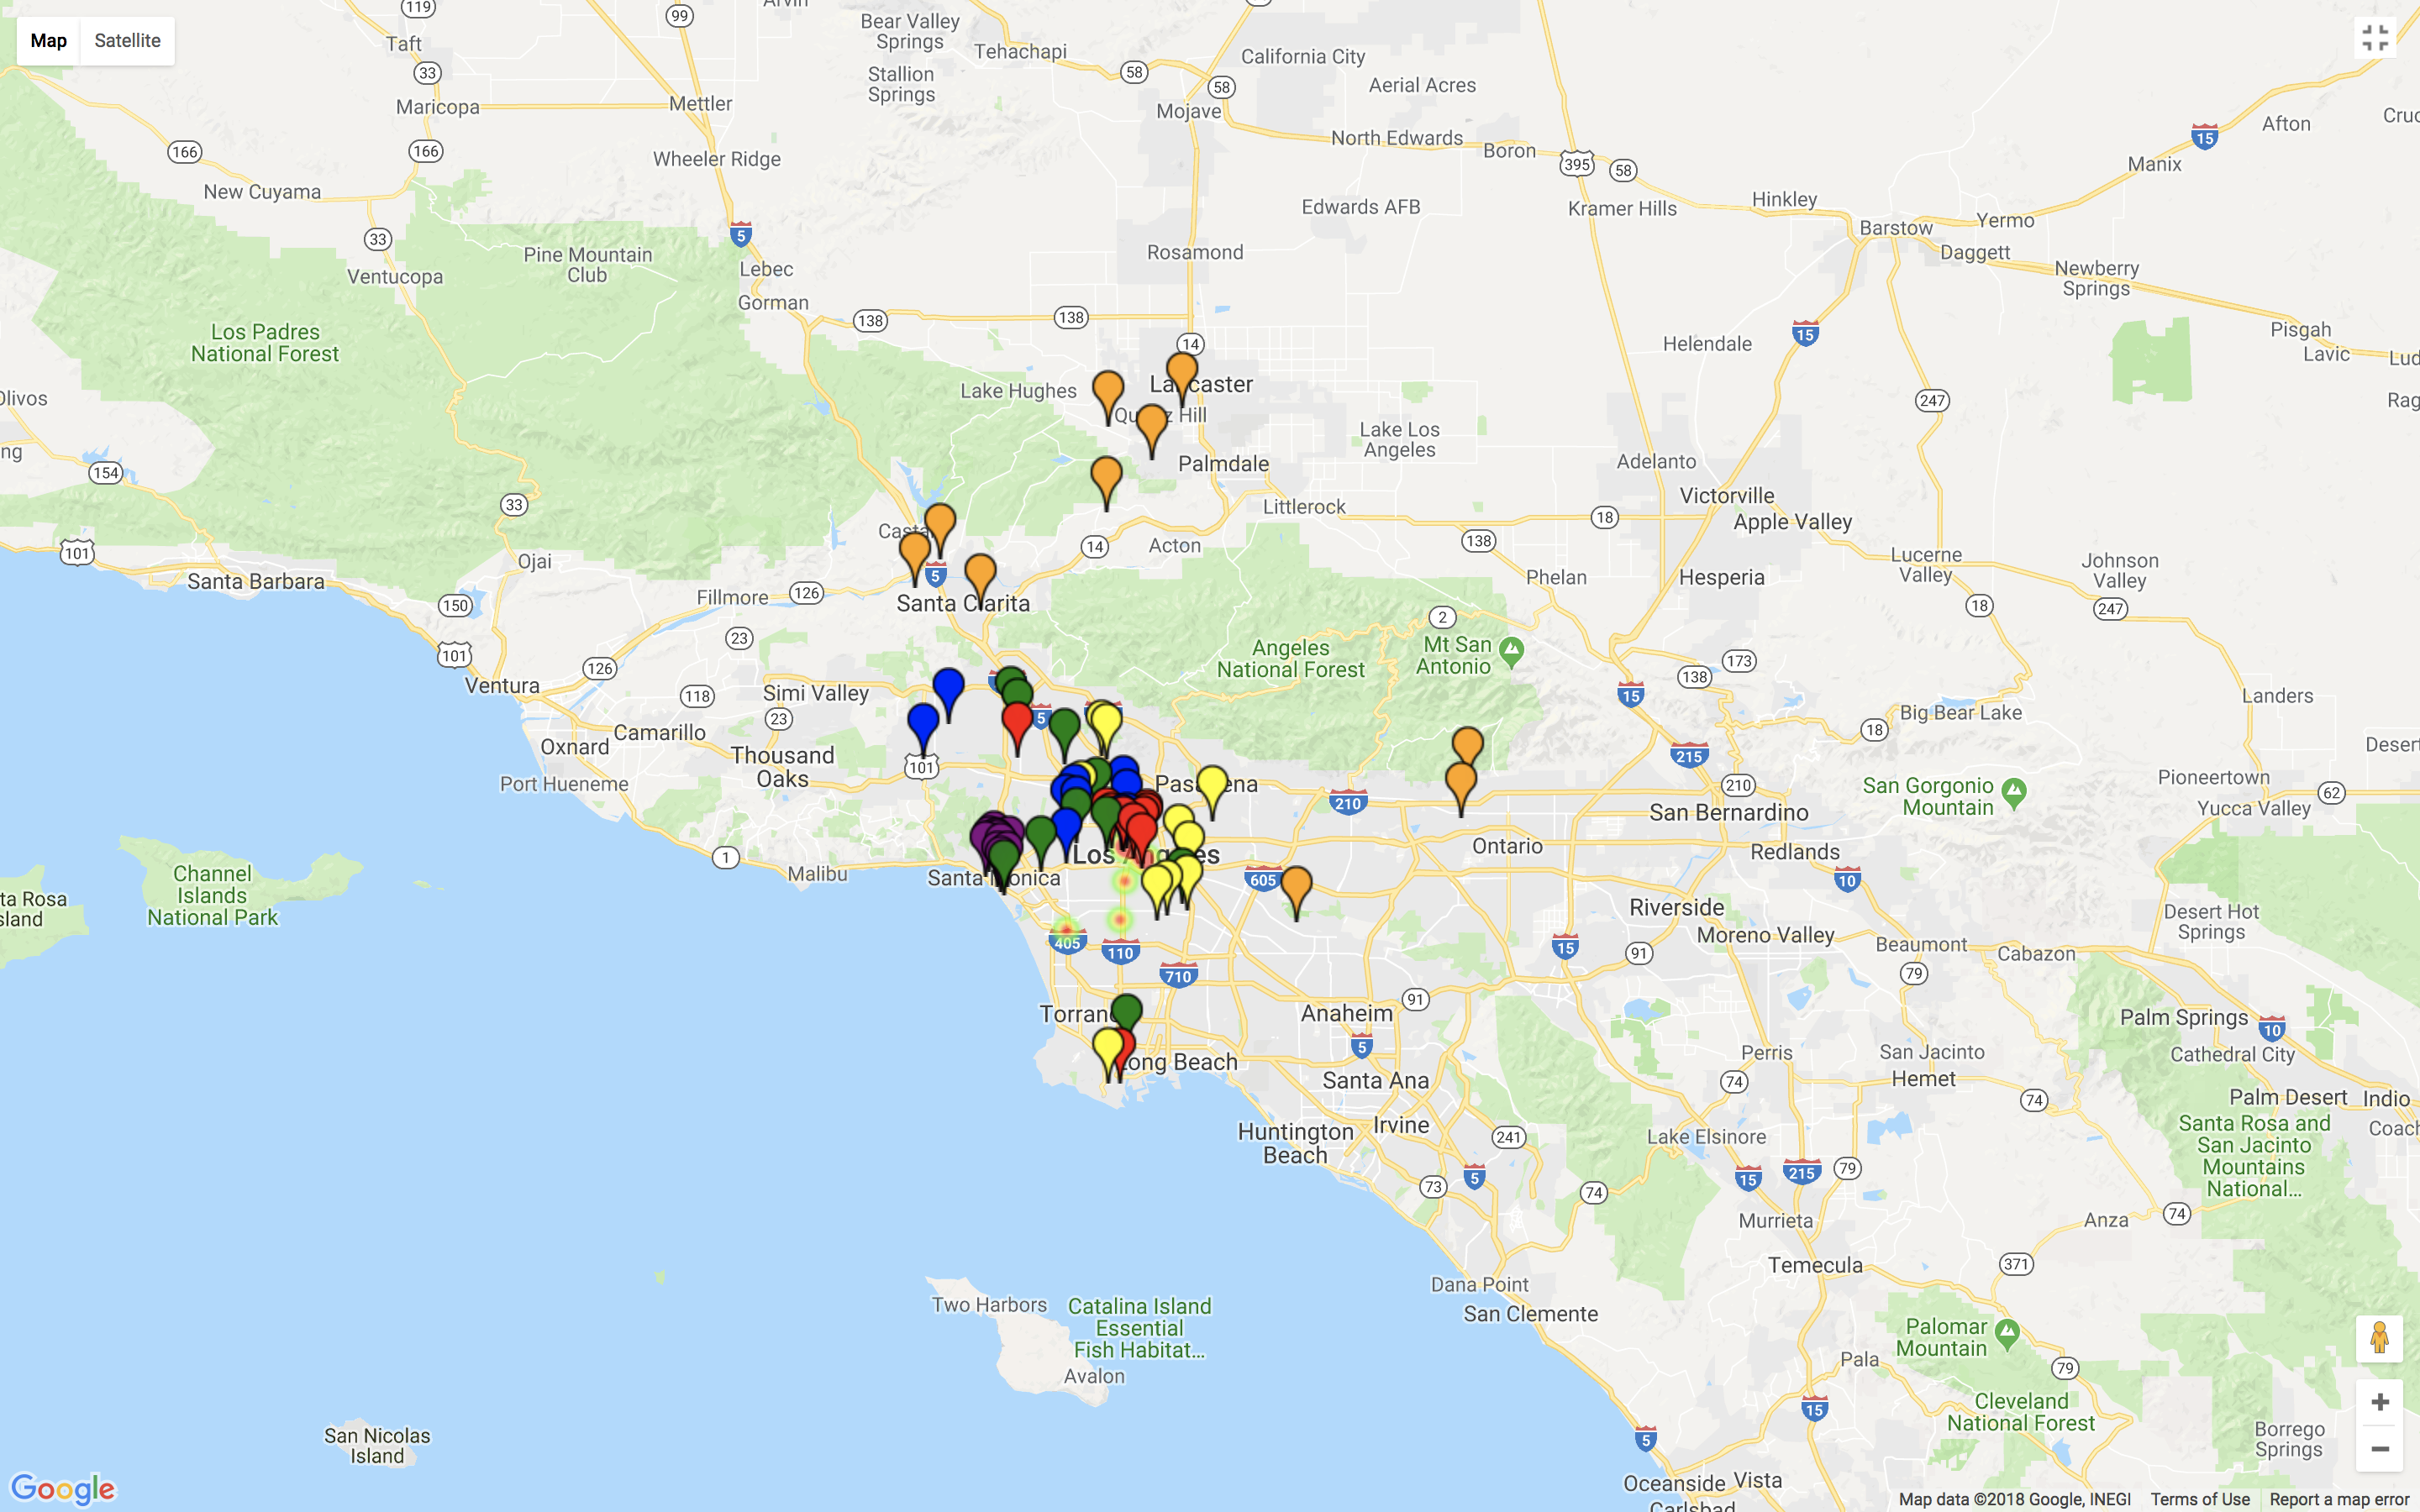
\includegraphics[width=\linewidth, height=0.4\textheight]{k=6.png}
  \caption{$k=6$}
\end{figure}
%
\begin{figure}[H]\centering
  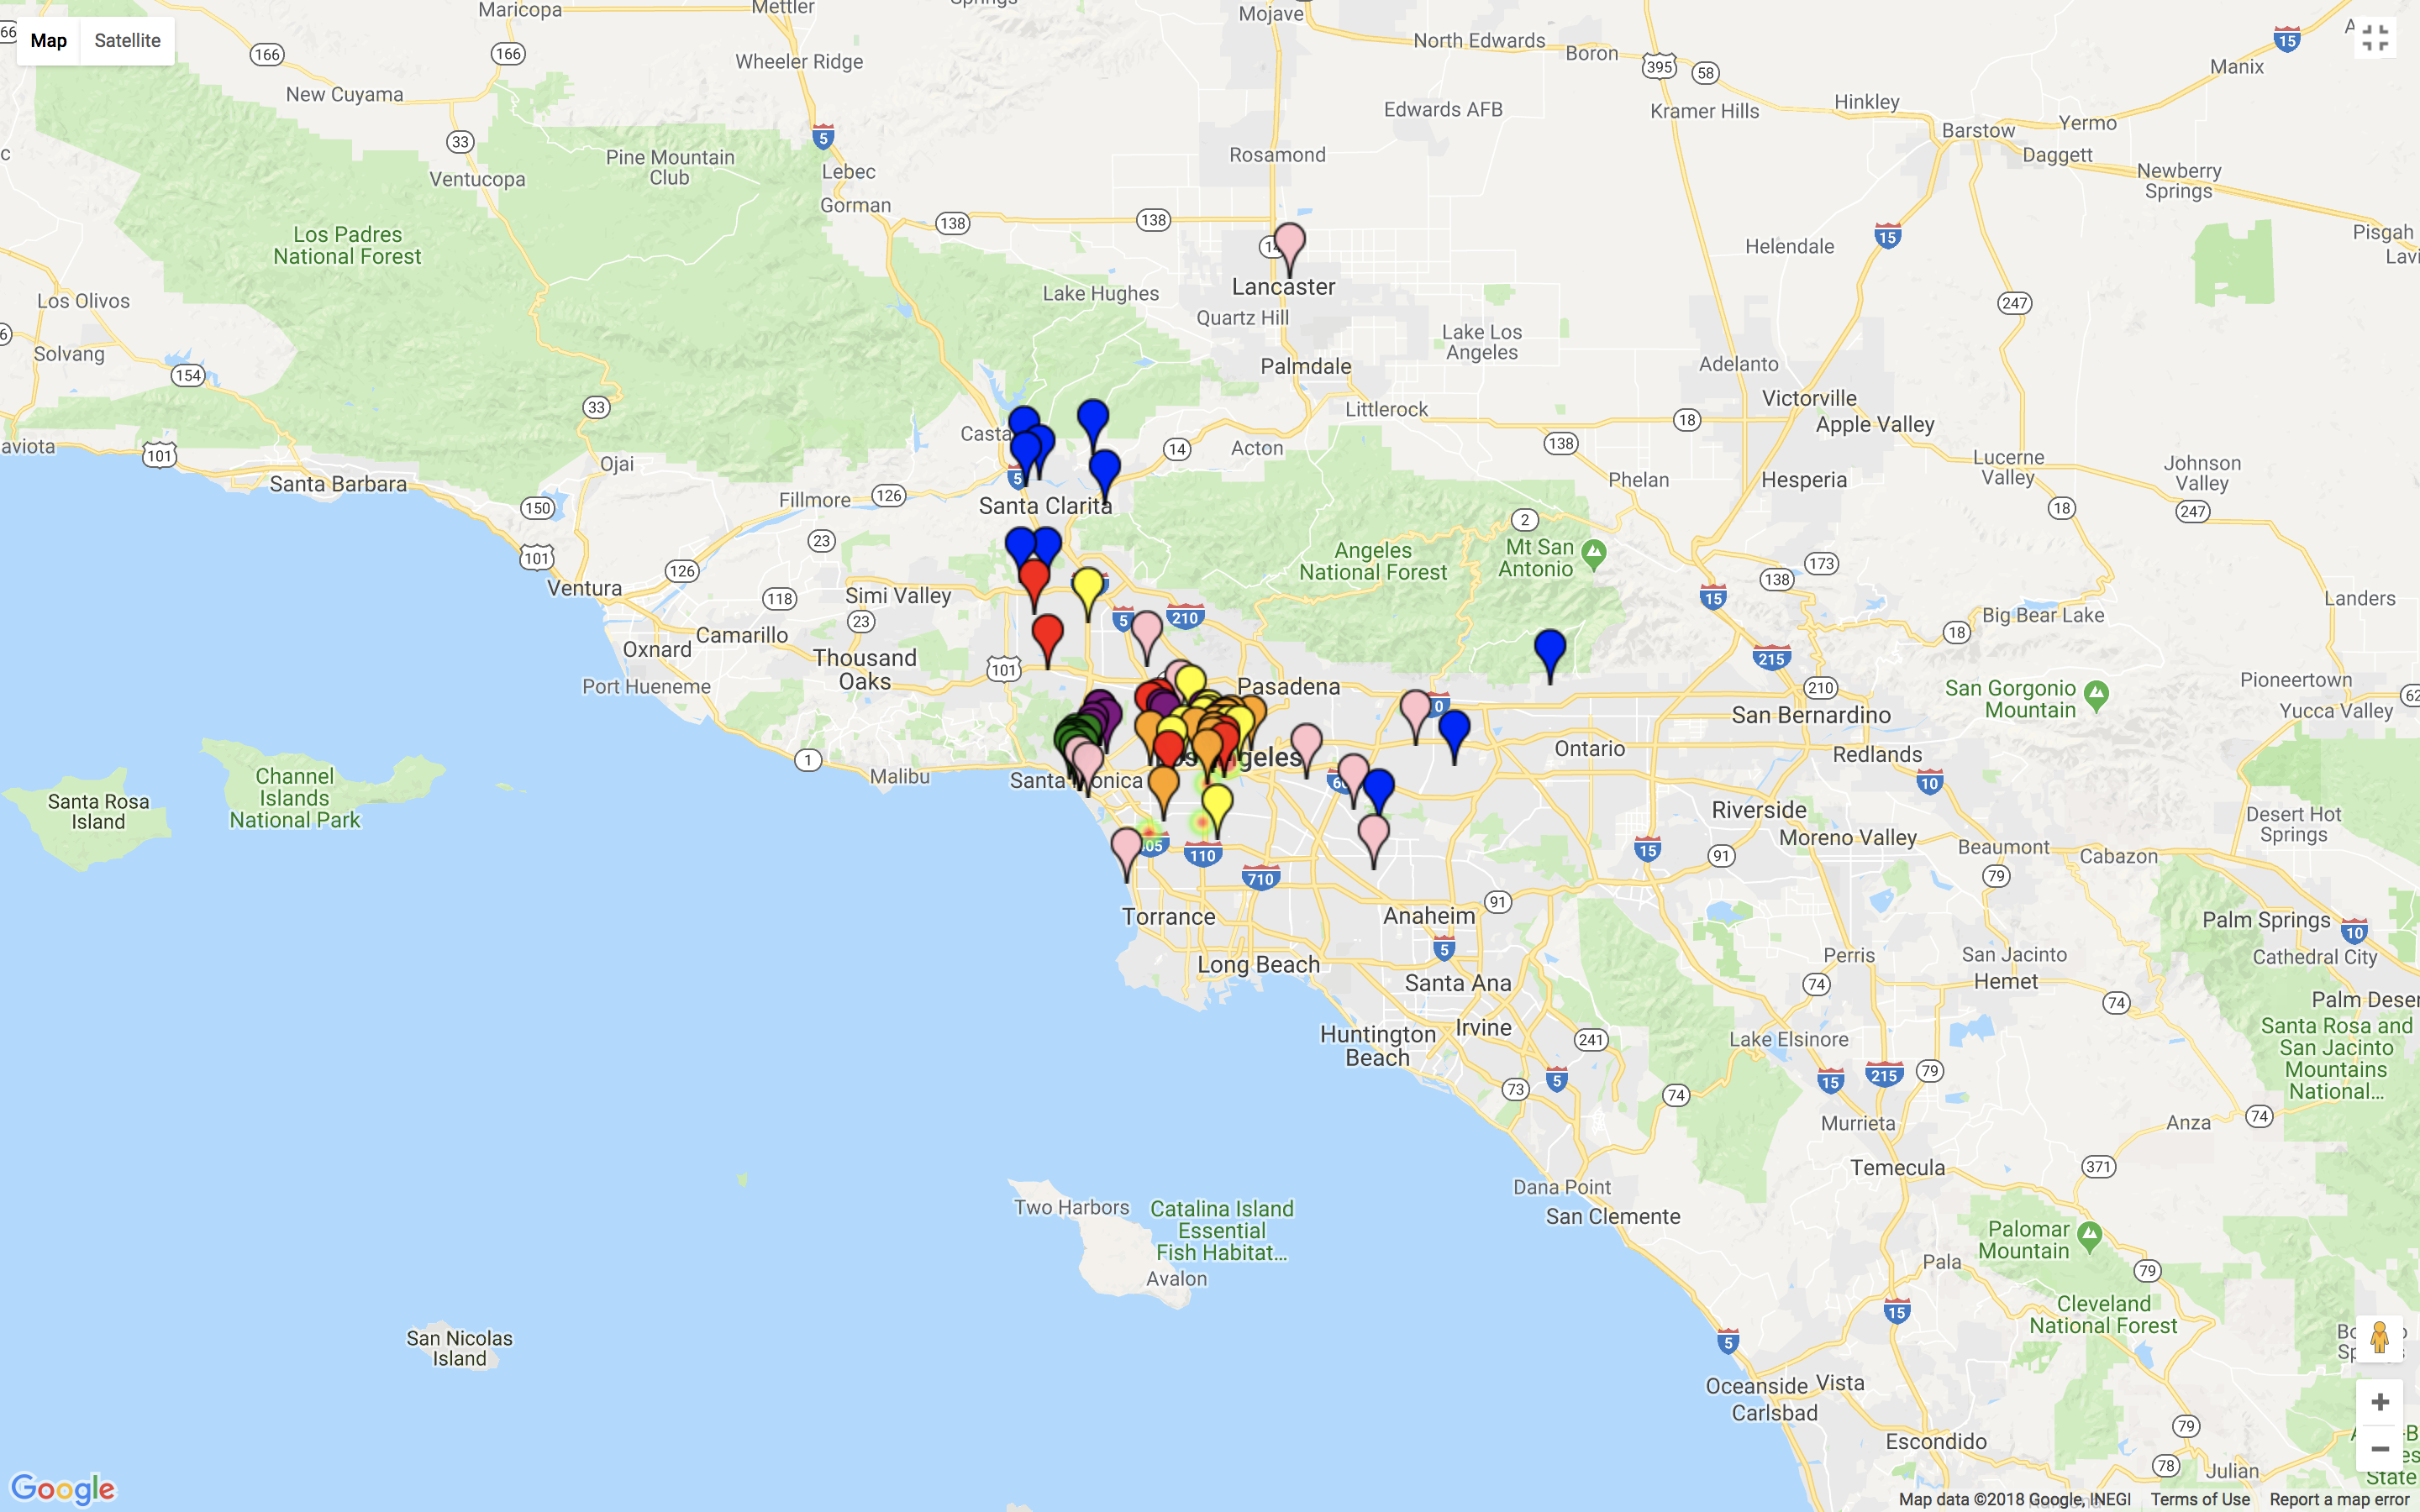
\includegraphics[width=\linewidth, height=0.4\textheight]{k=7.png}
  \caption{$k=7$}
\end{figure}
%
\begin{figure}[H]
  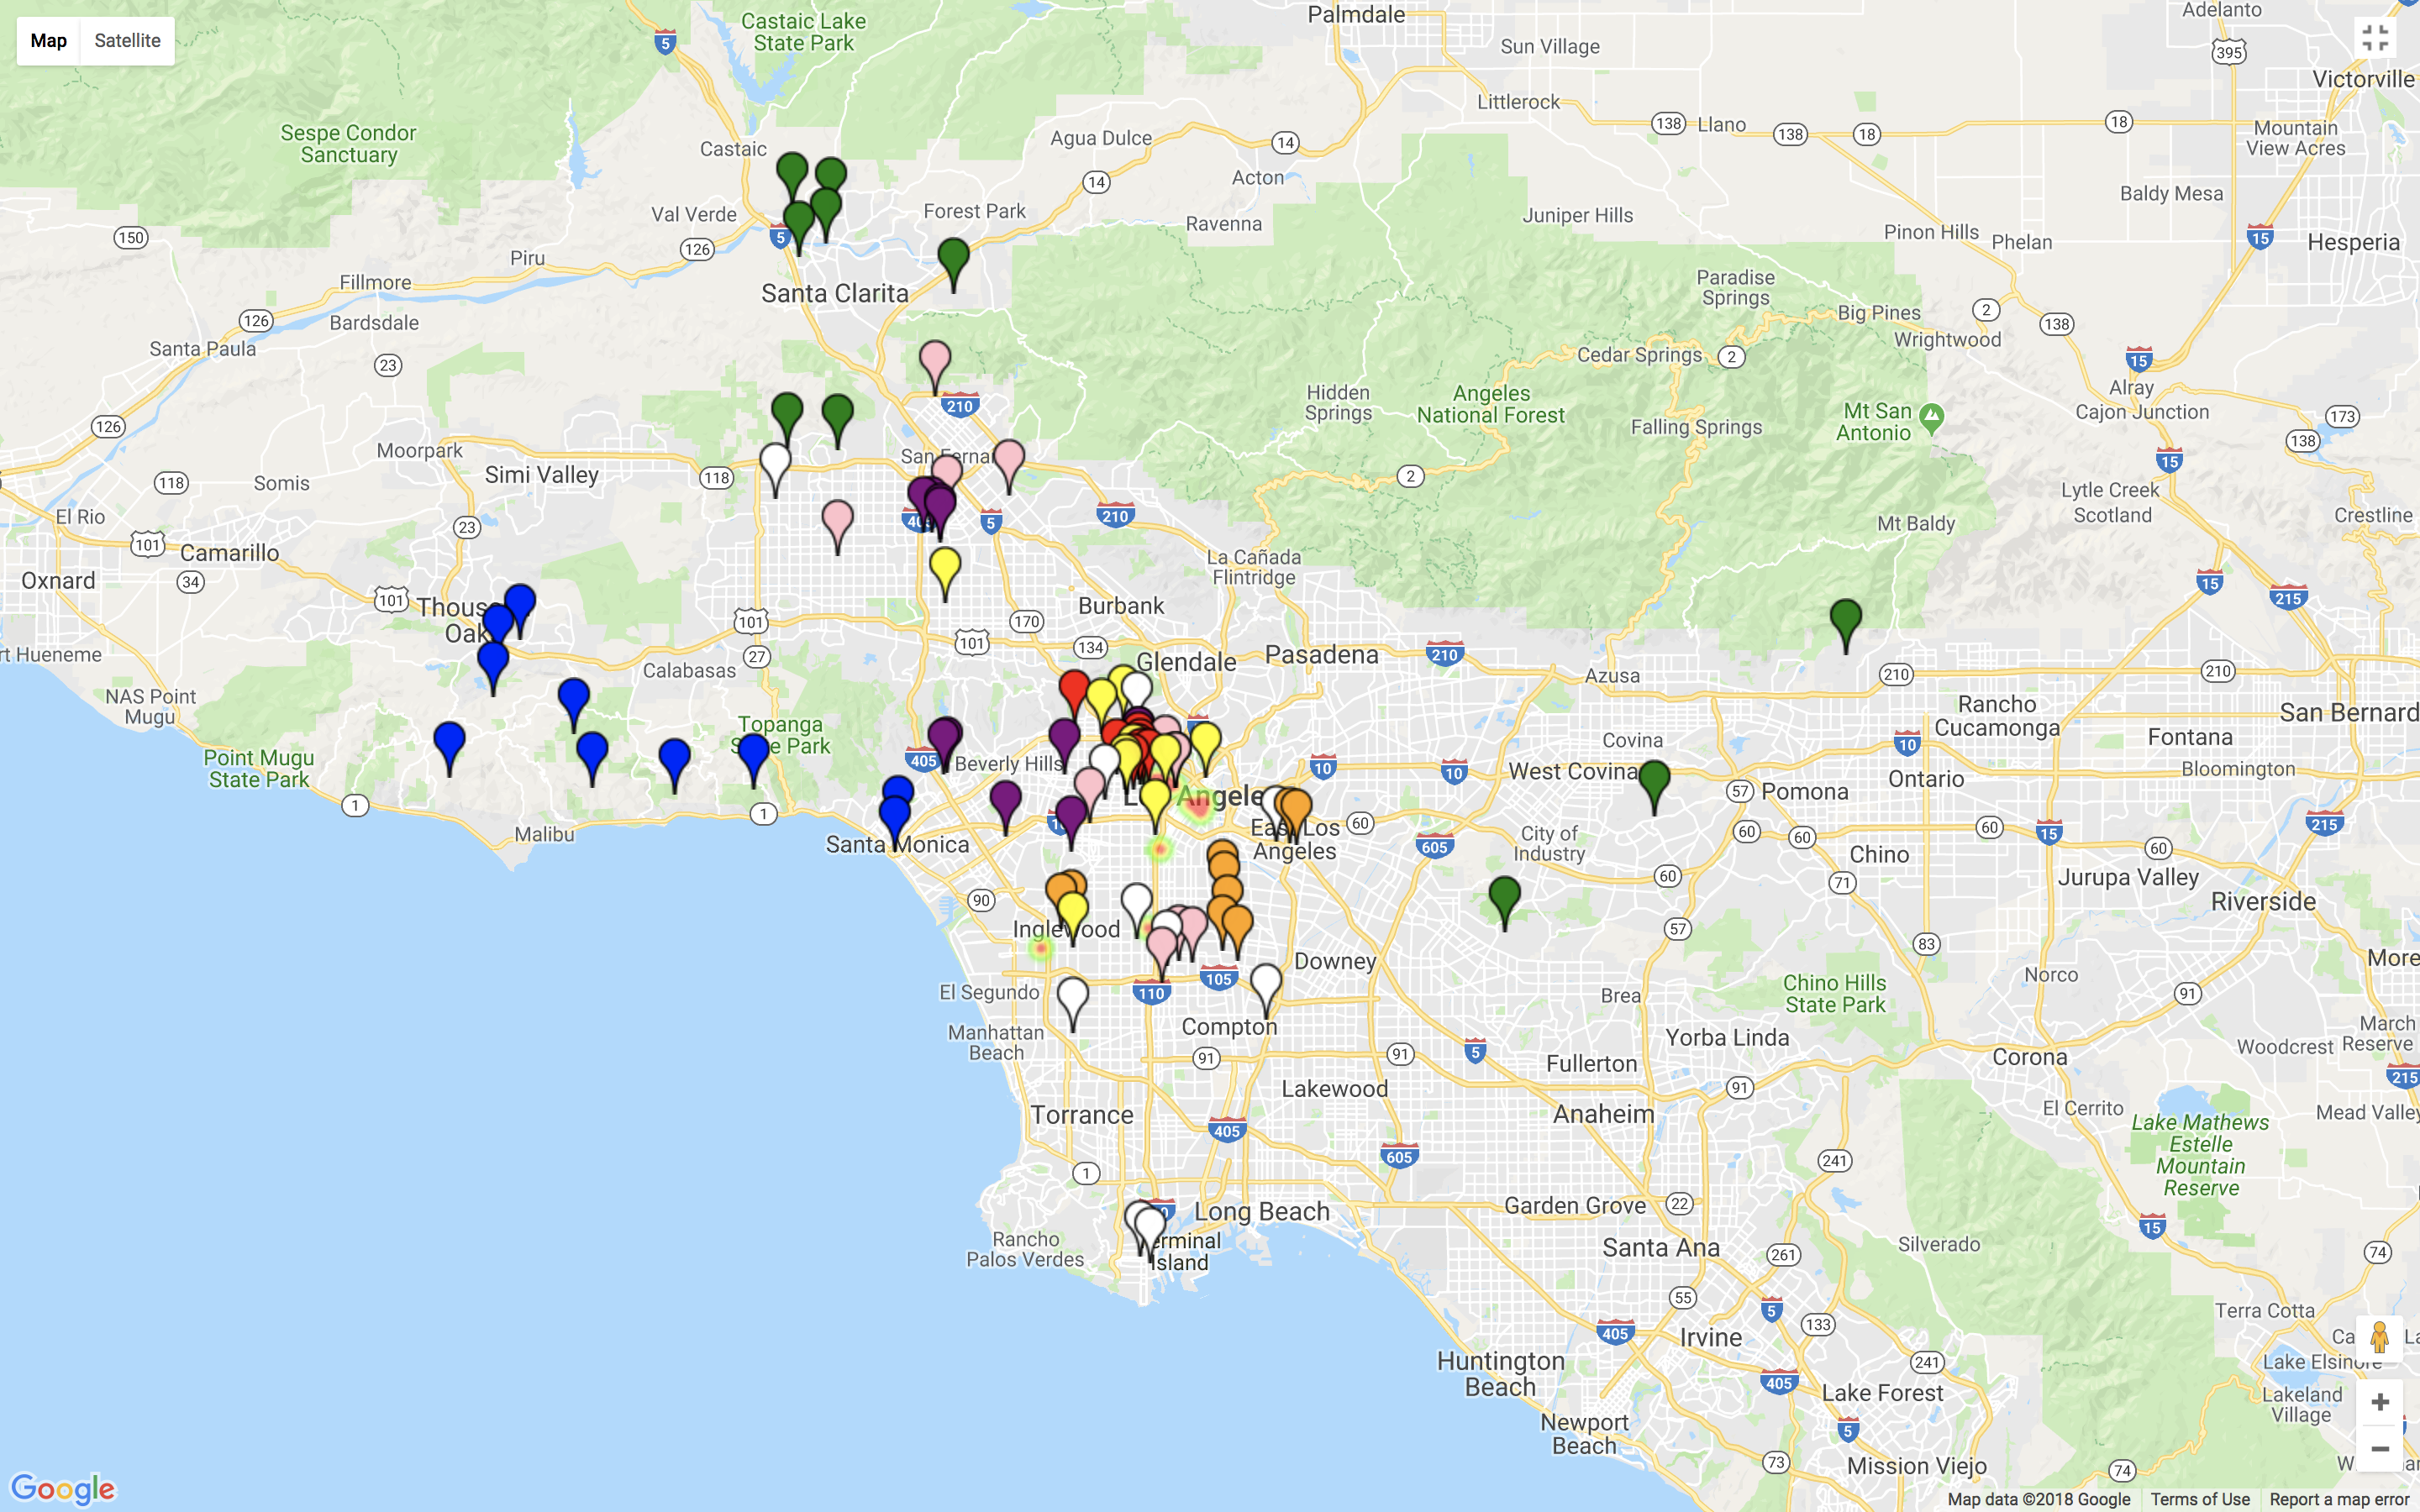
\includegraphics[width=\linewidth, height=0.4\textheight]{k=8.png}
  \caption{$k=8$}
\end{figure}
\end{subfigures}



%
\begin{comment}
\begin{figure}[H]
  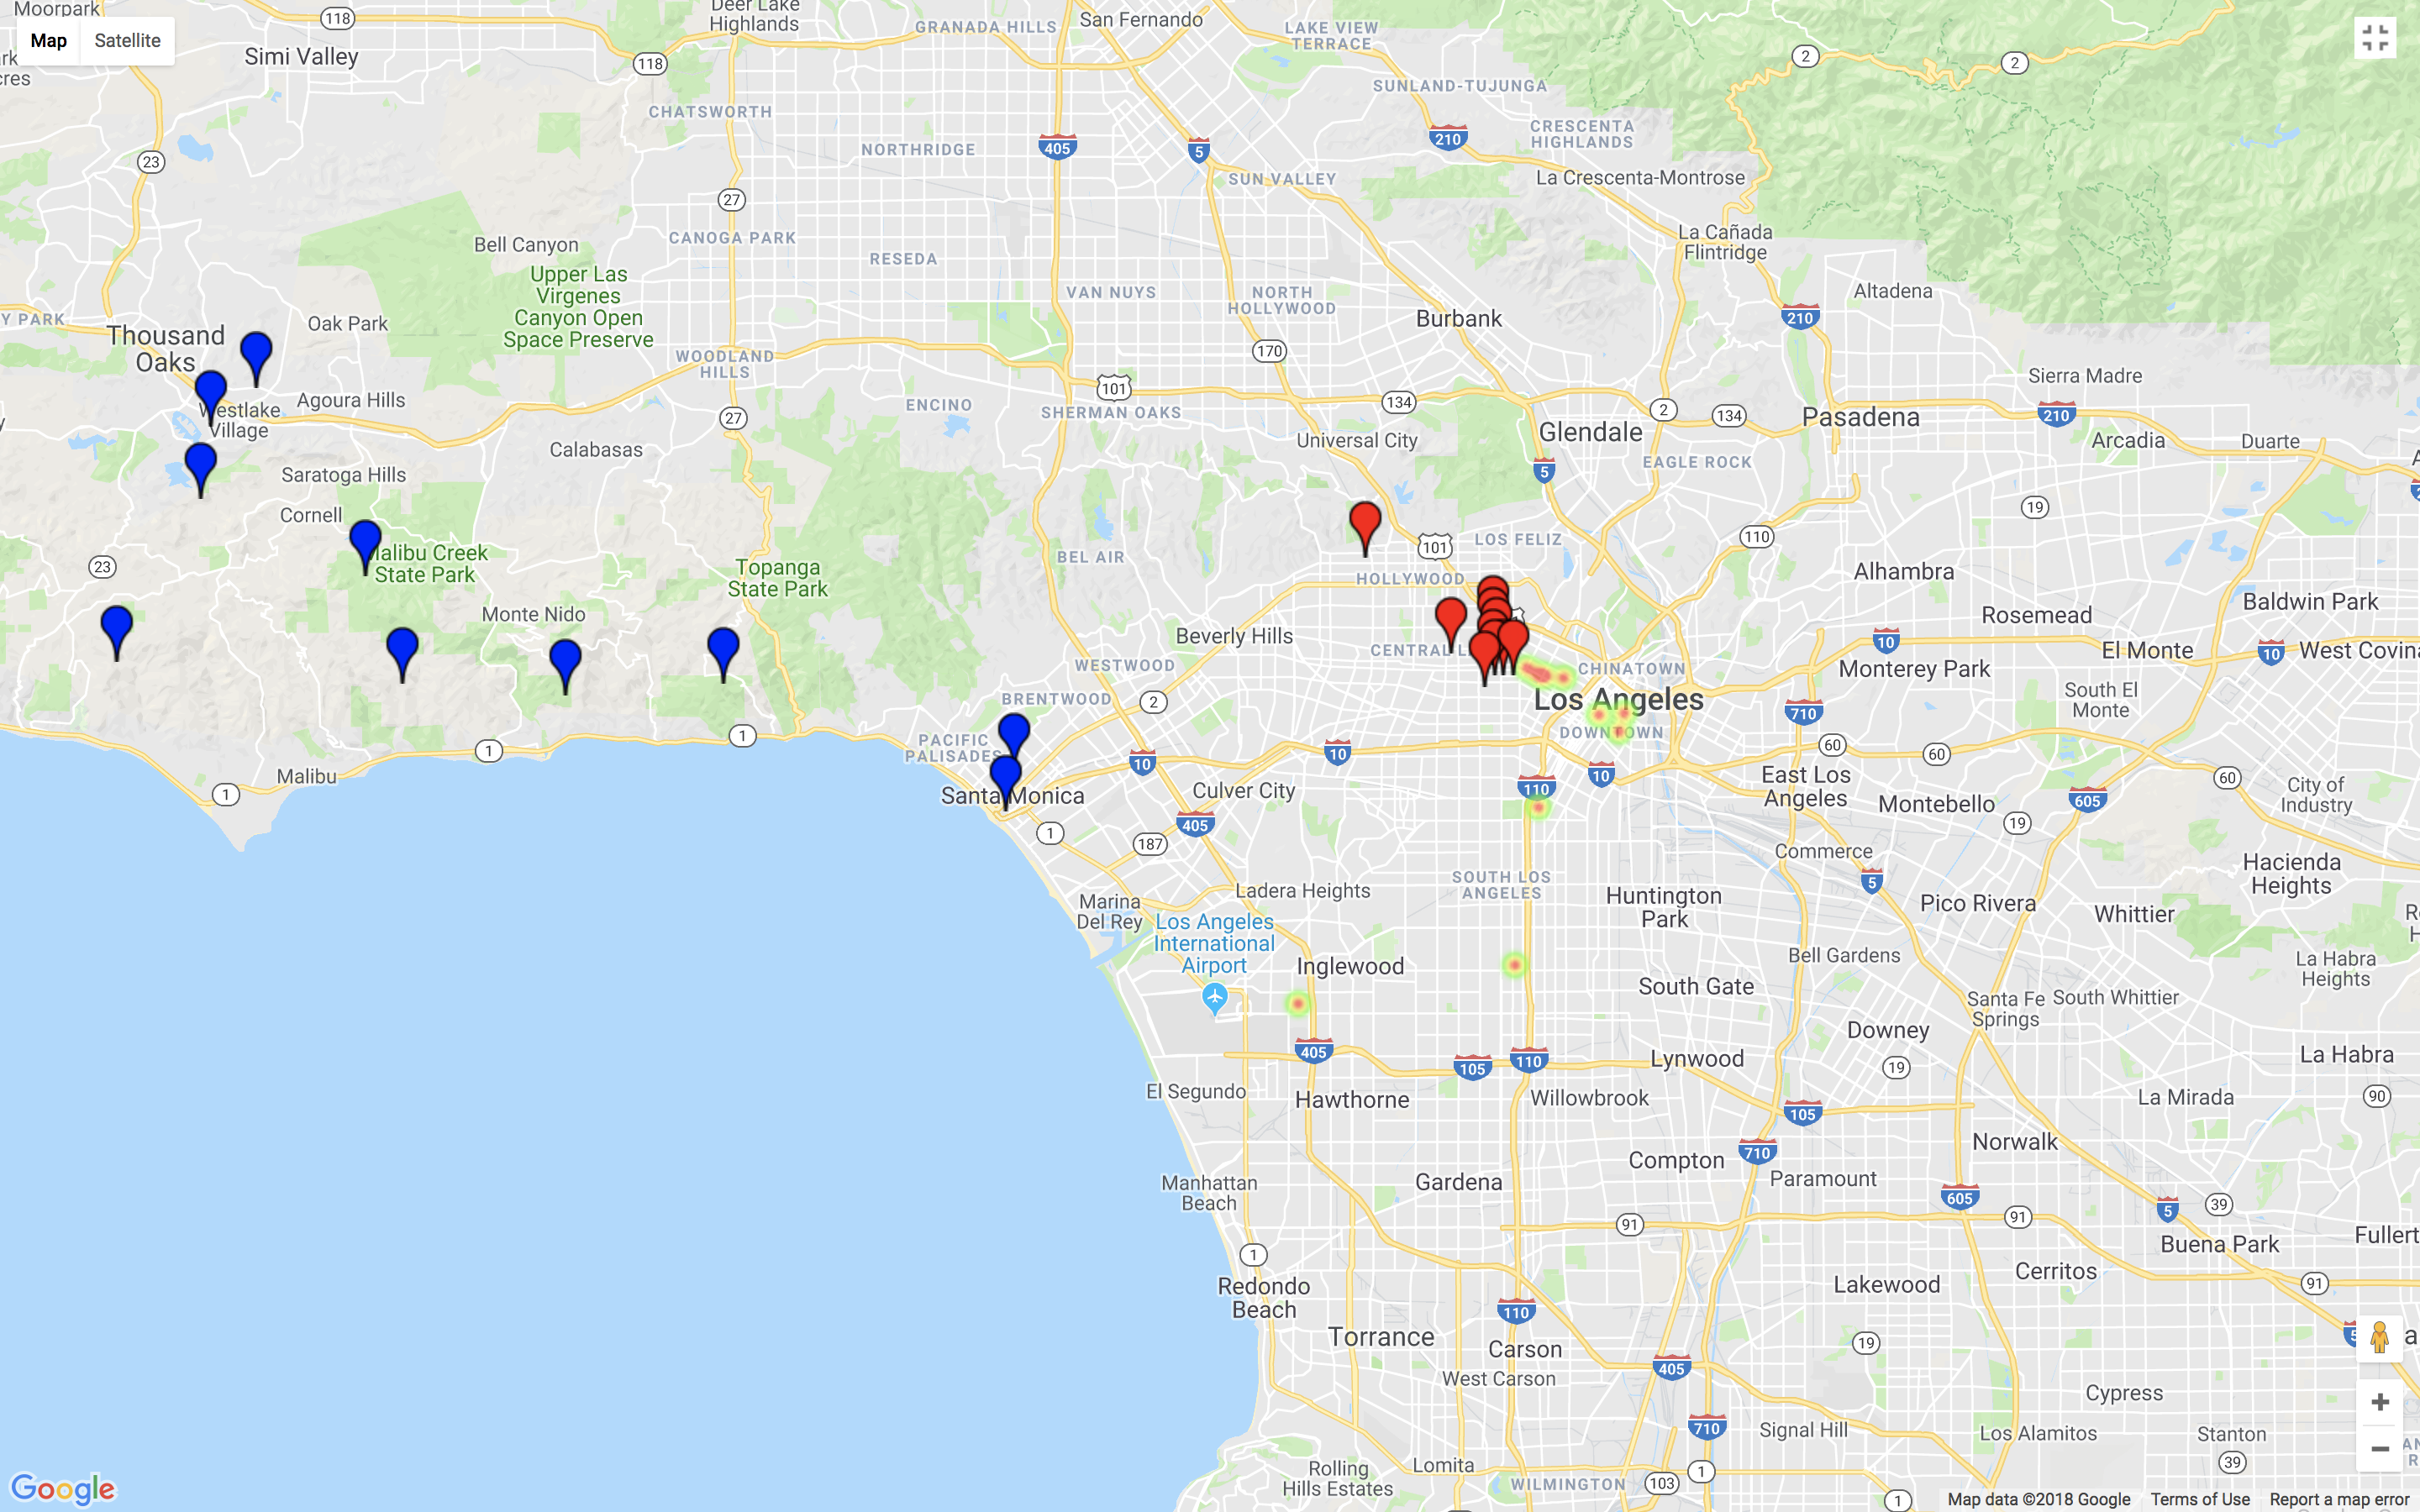
\includegraphics[width=\linewidth]{k=2.png}
  
\end{figure}

\begin{figure}[H]
  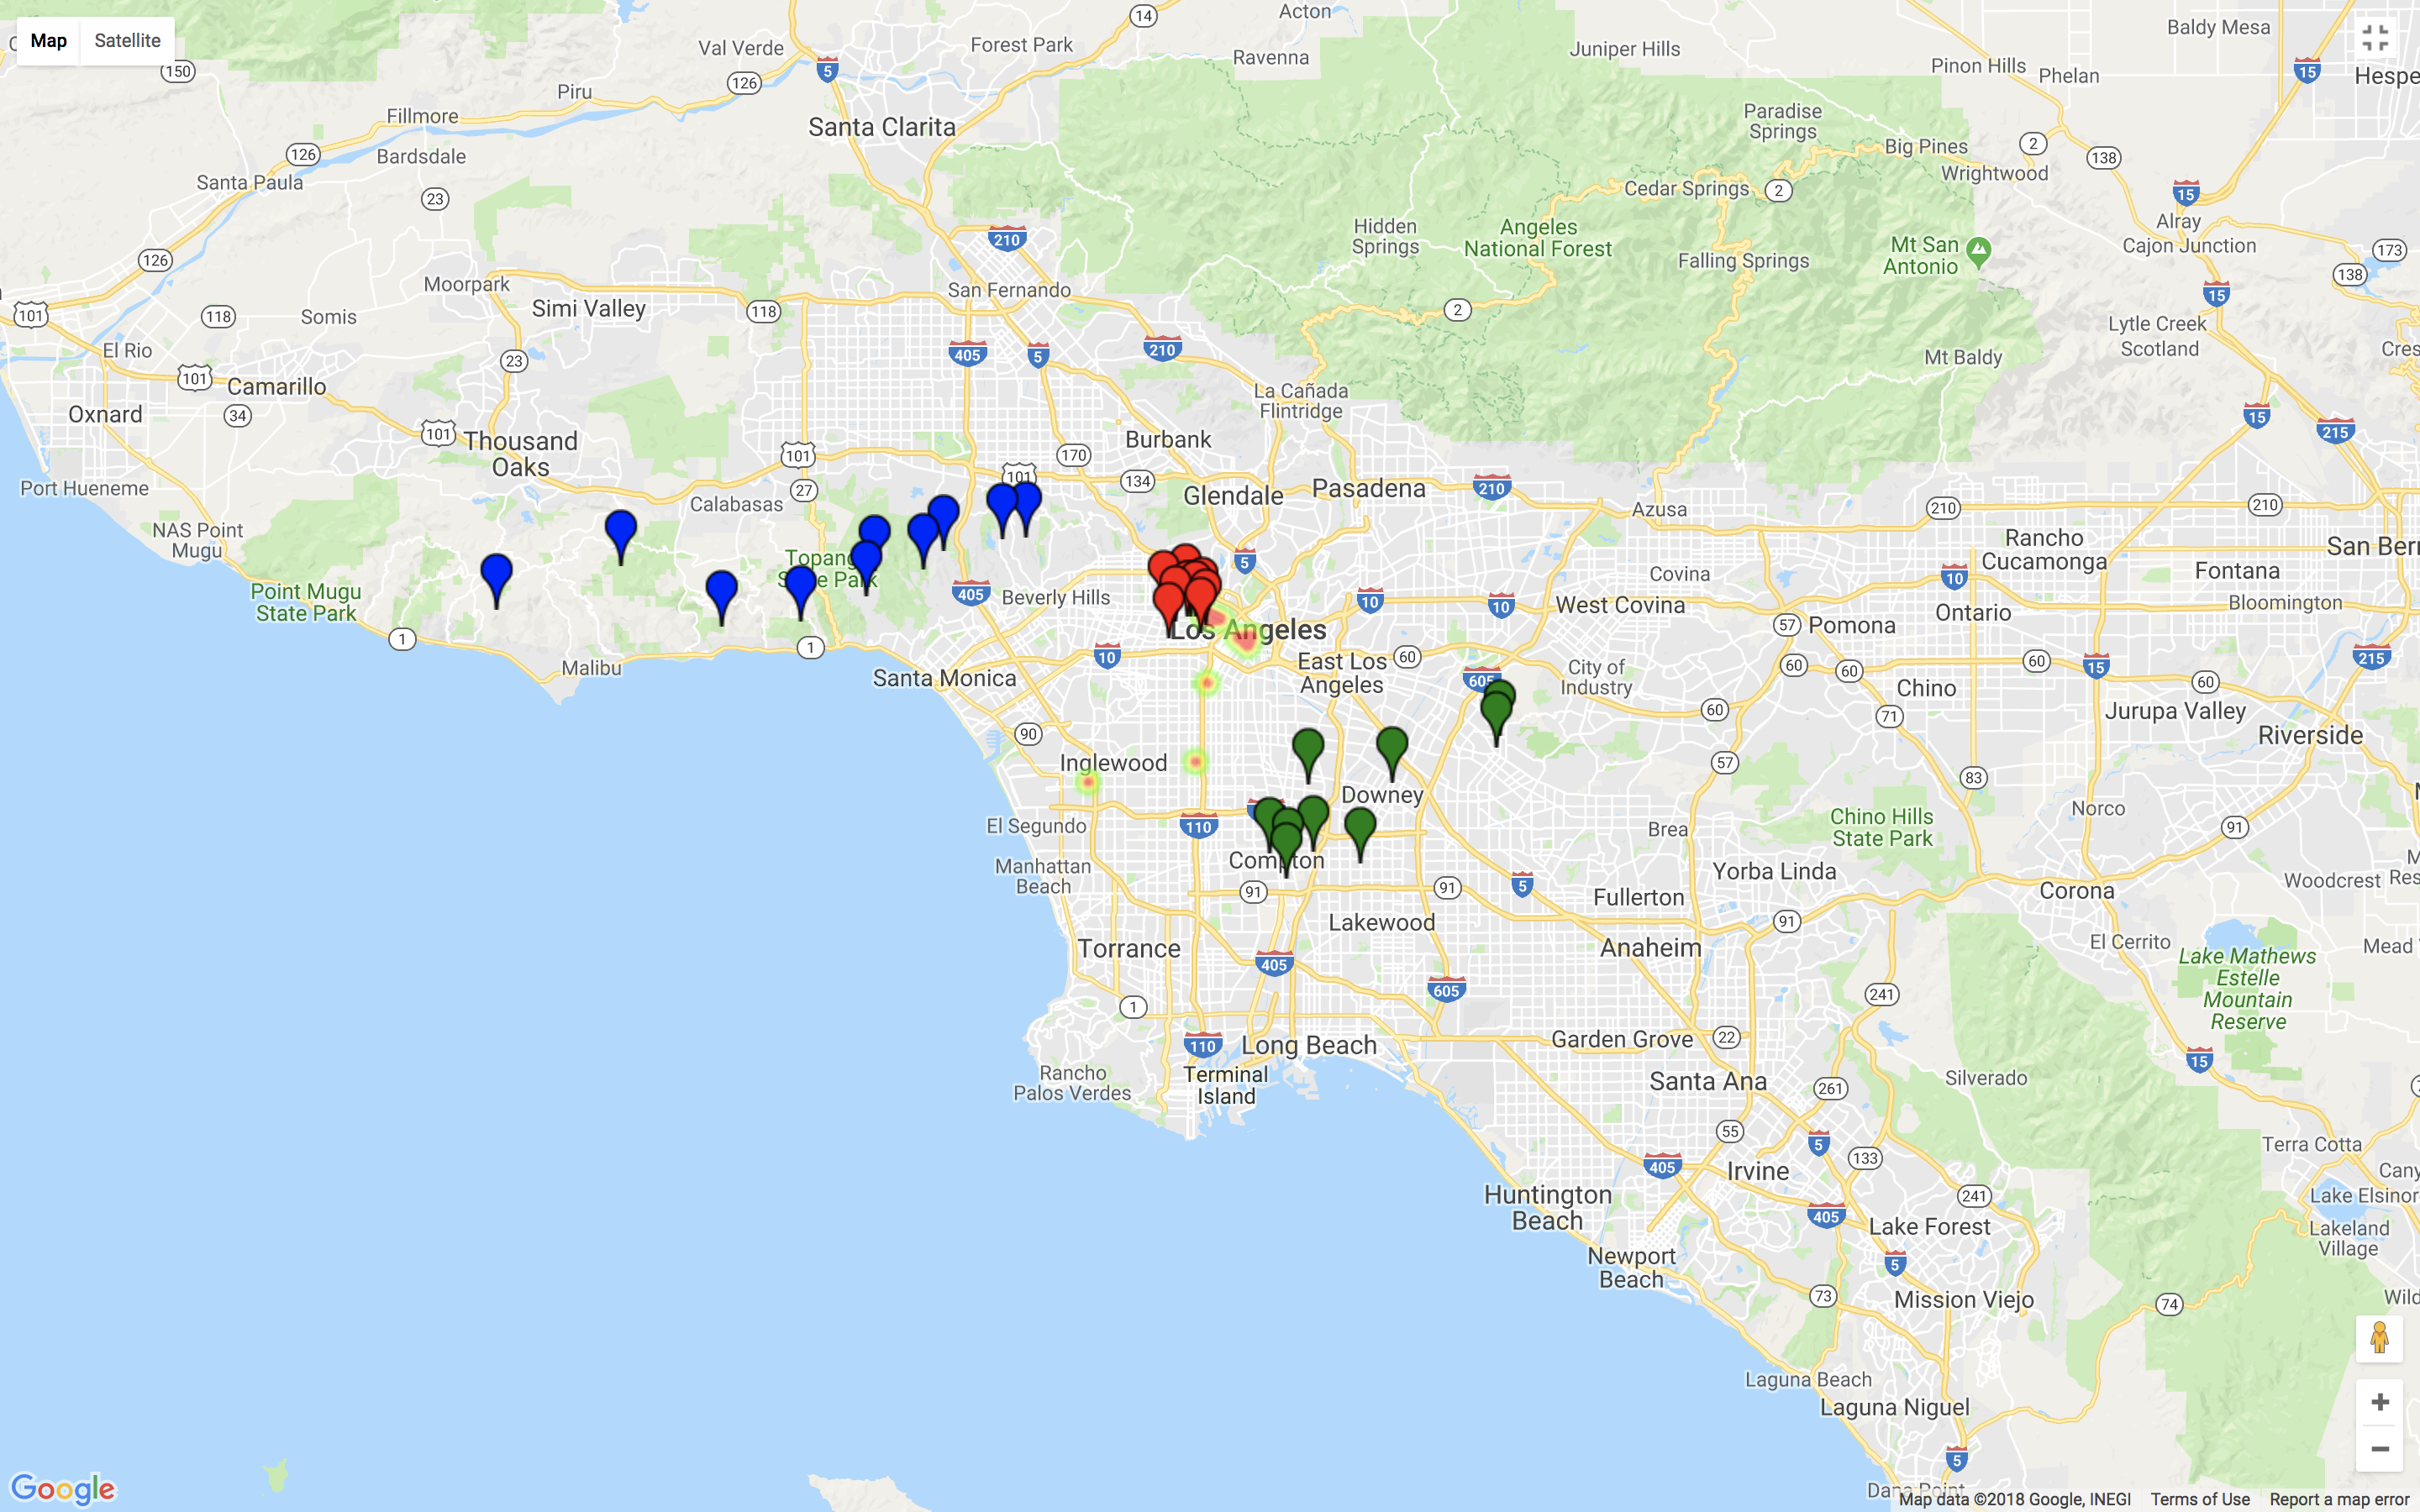
\includegraphics[width=\linewidth]{k=3.png}
  \caption{$k=3$}
\end{figure}

\begin{figure}[H]
  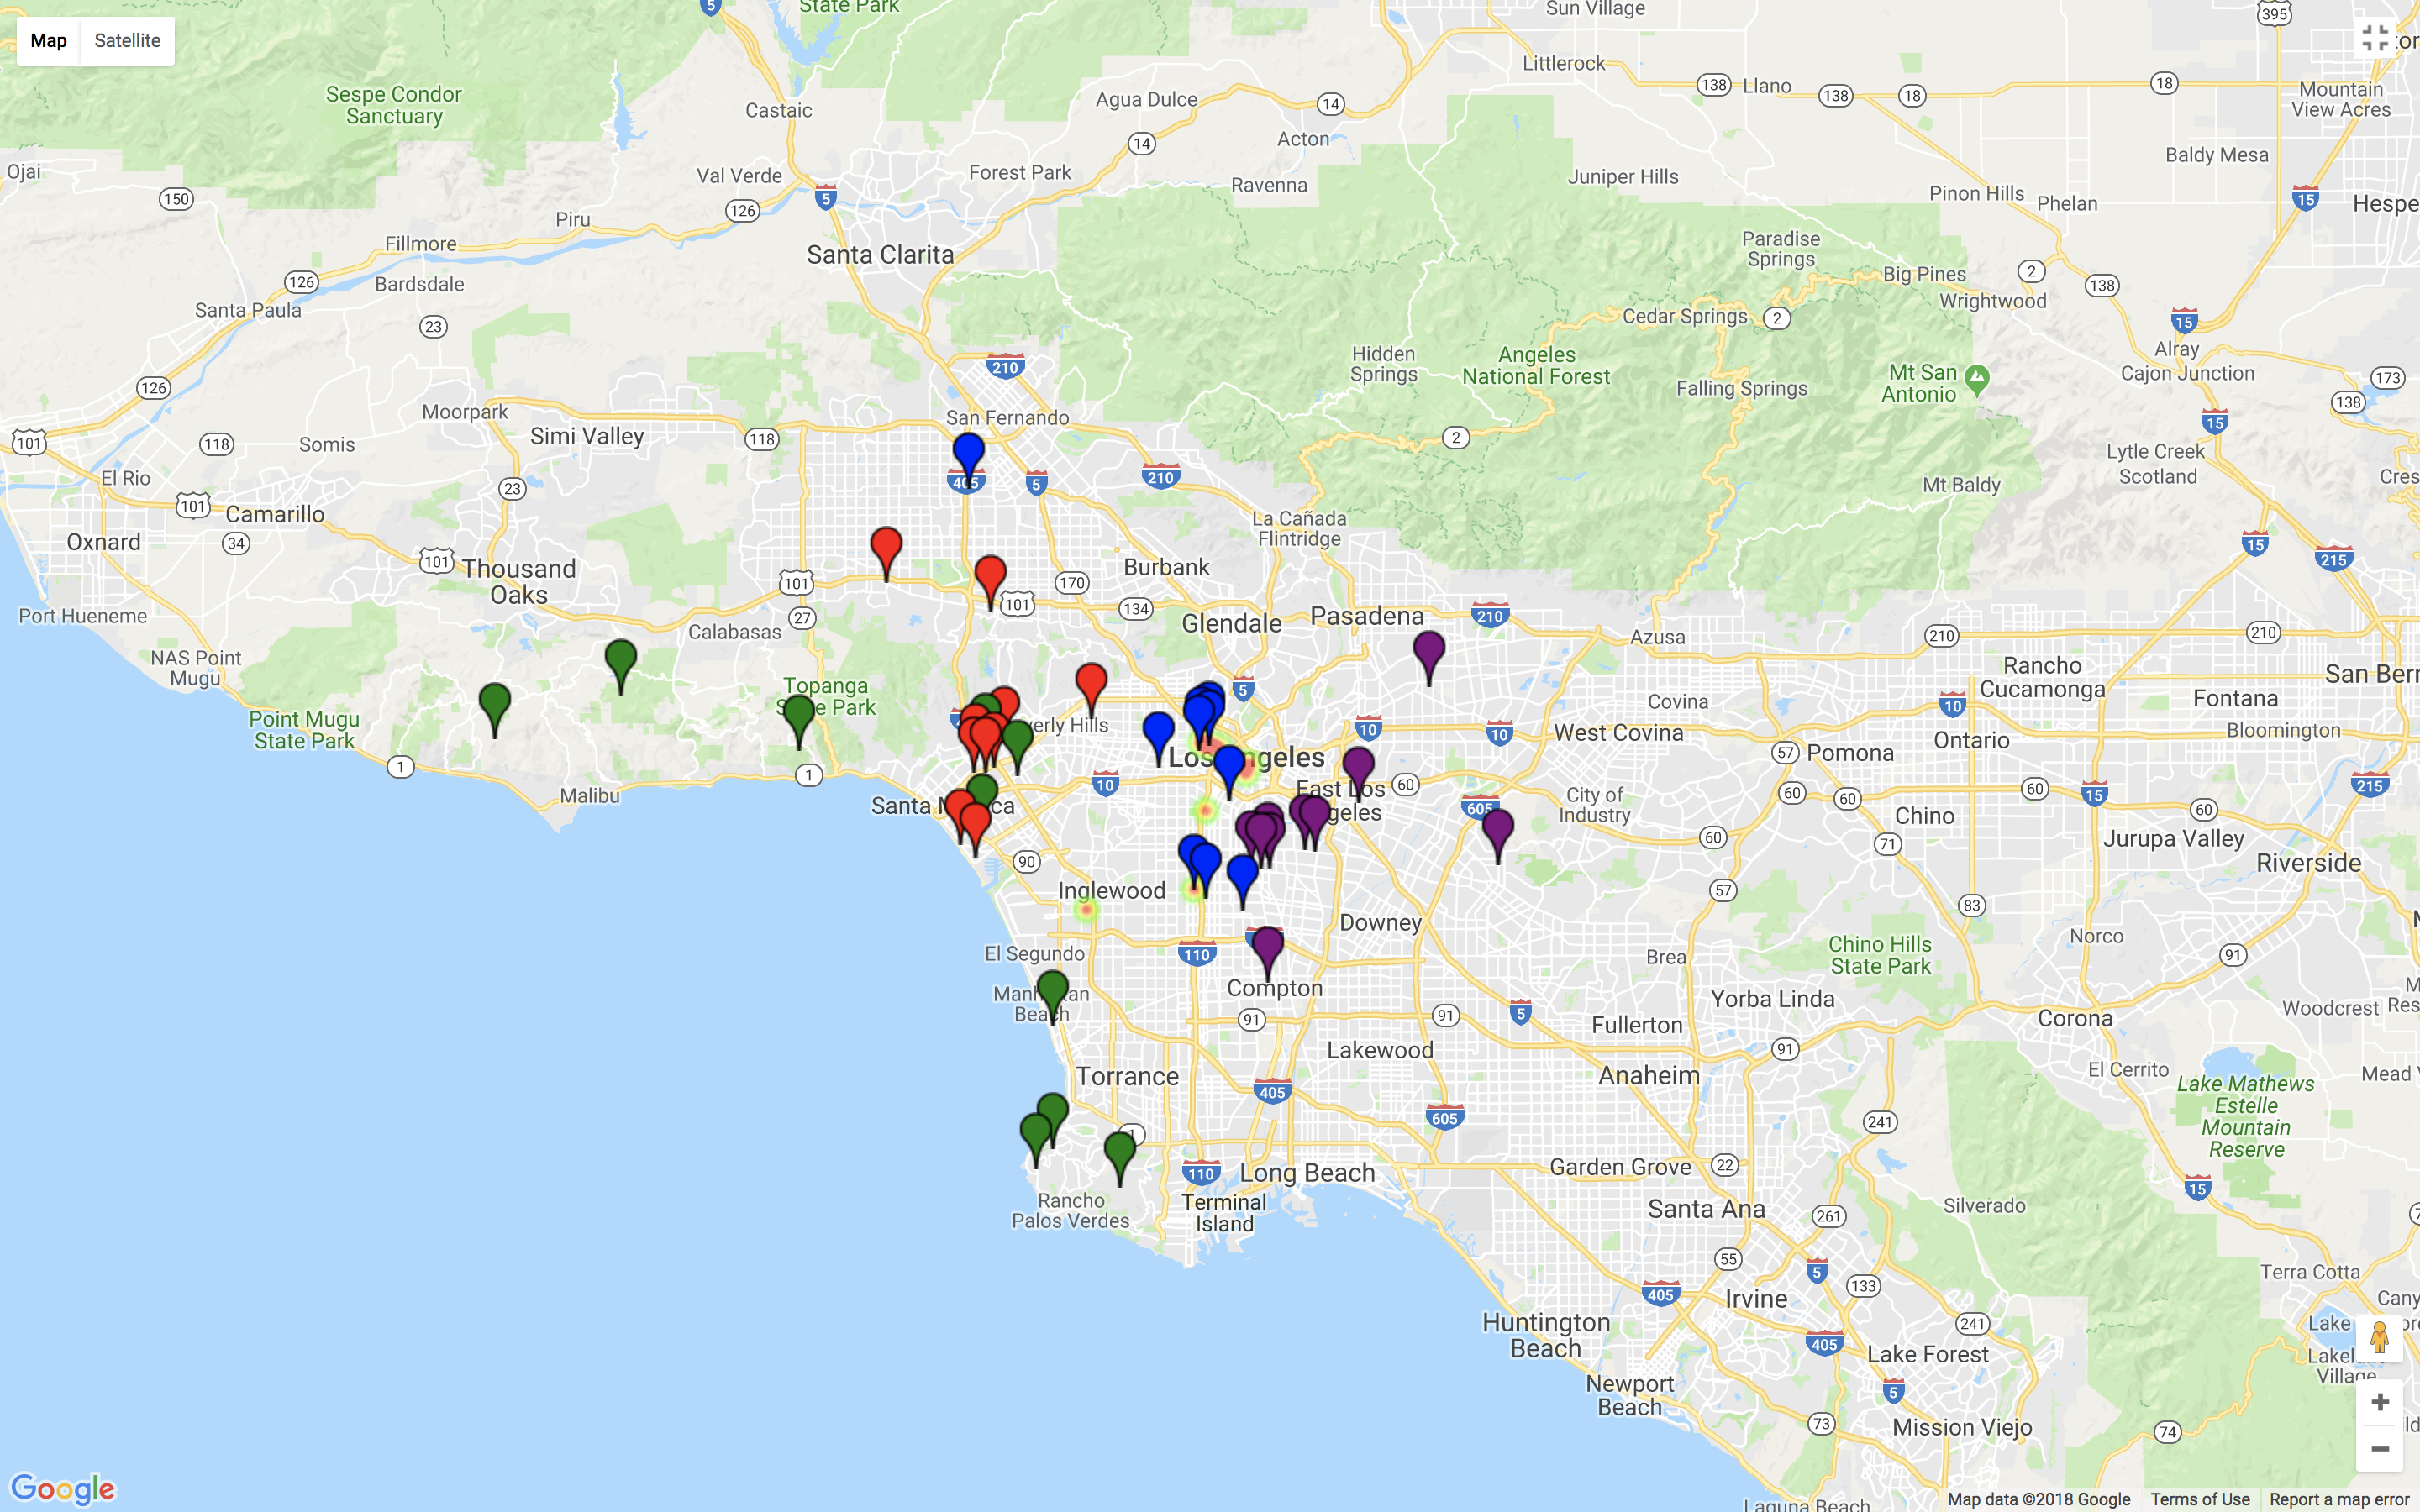
\includegraphics[width=\linewidth]{k=4.png}
  \caption{$k=4$}
\end{figure}

\begin{figure}[H]
  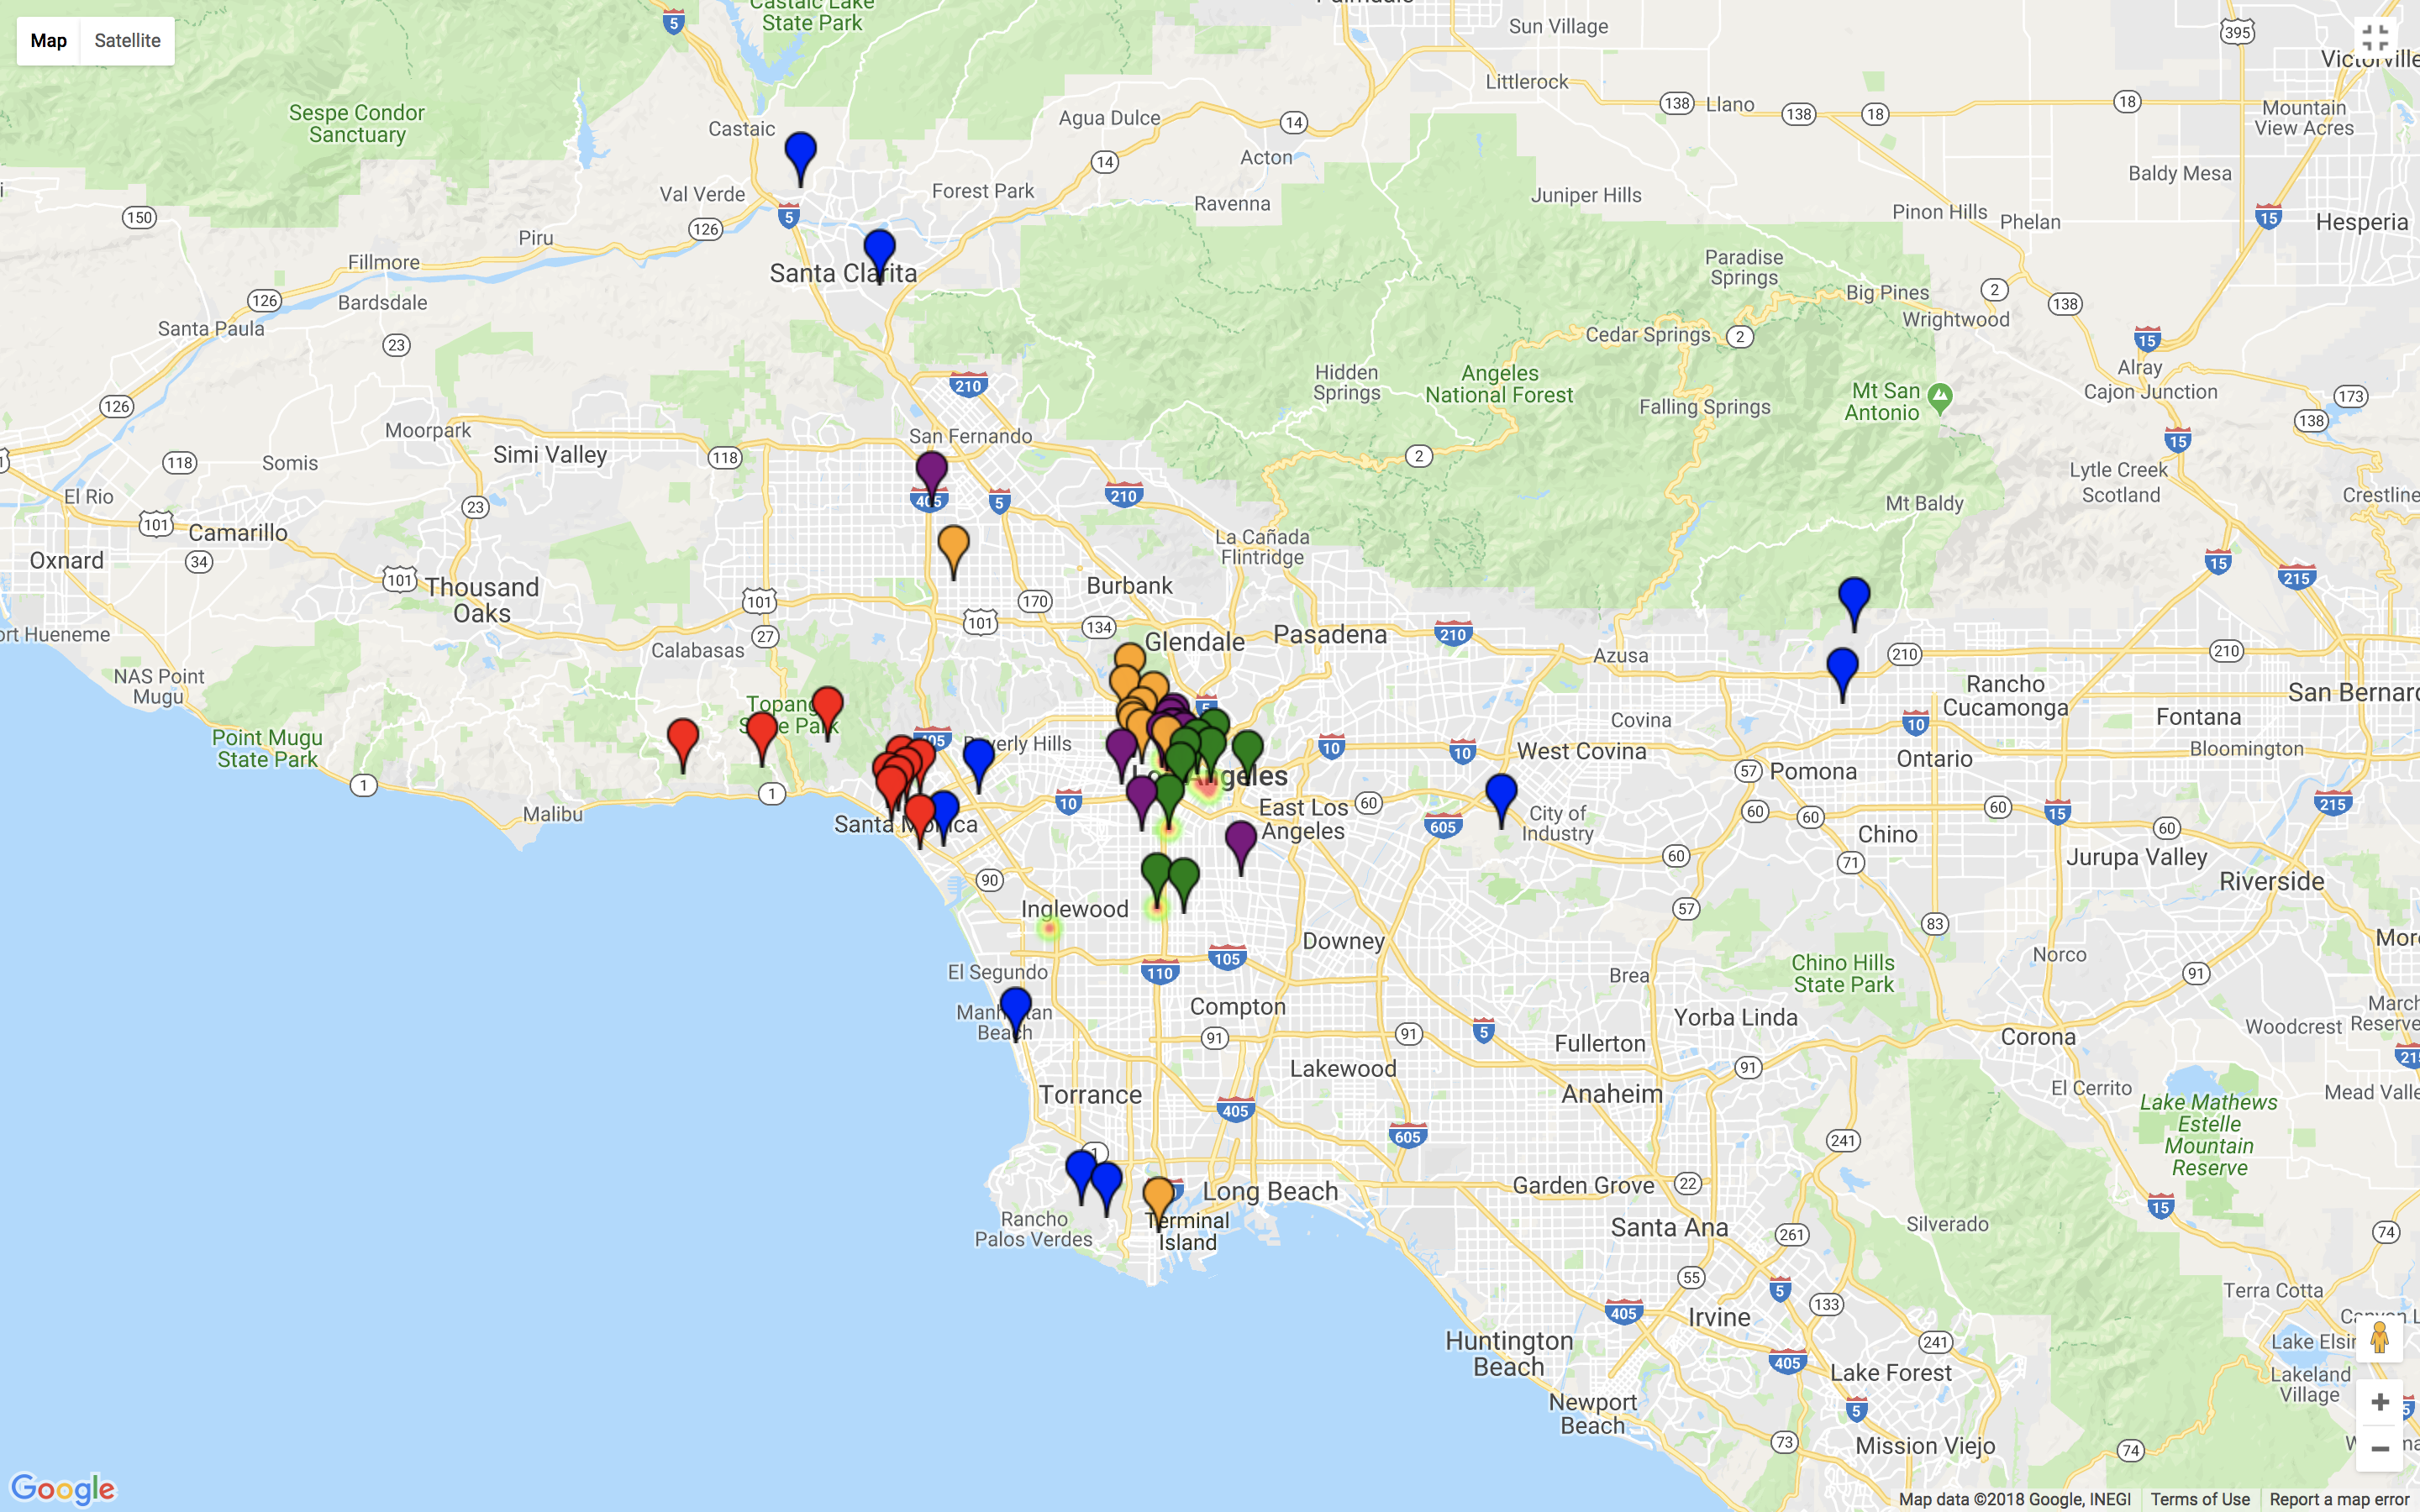
\includegraphics[width=\linewidth]{k=5.png}
  \caption{$k=5$}
\end{figure}

\begin{figure}[H]
  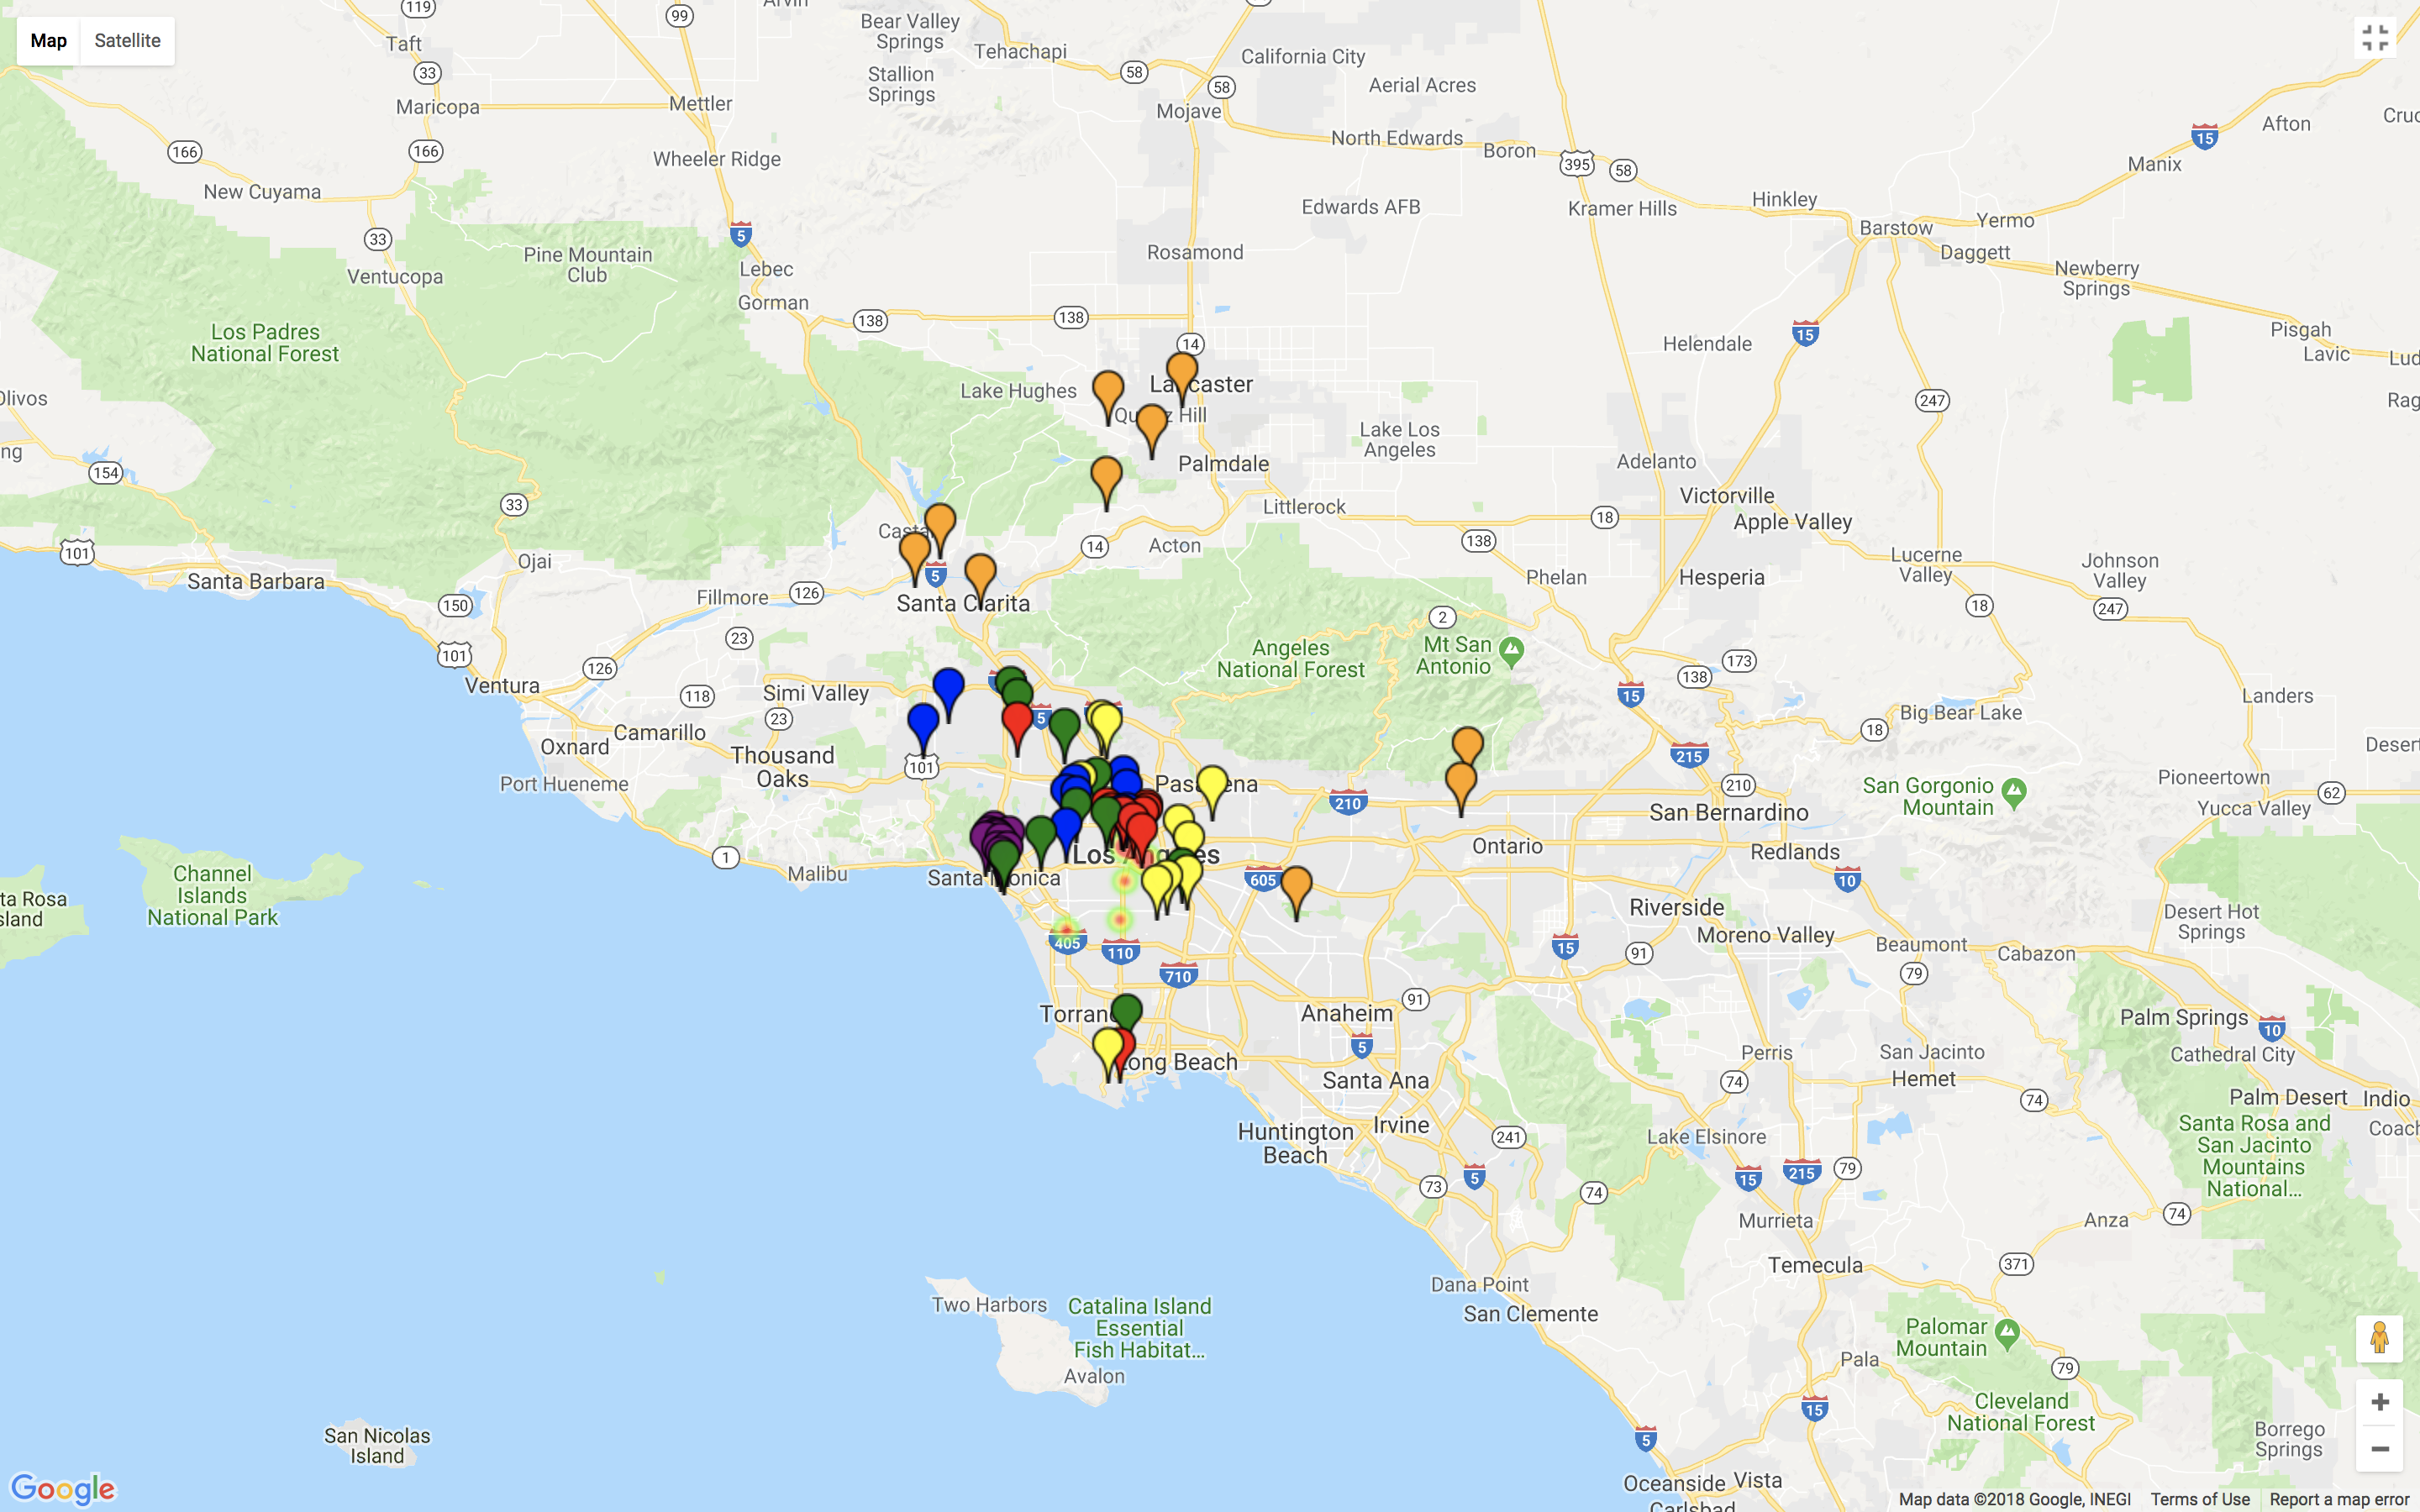
\includegraphics[width=\linewidth]{k=6.png}
  \caption{$k=6$}
\end{figure}

\begin{figure}[H]
  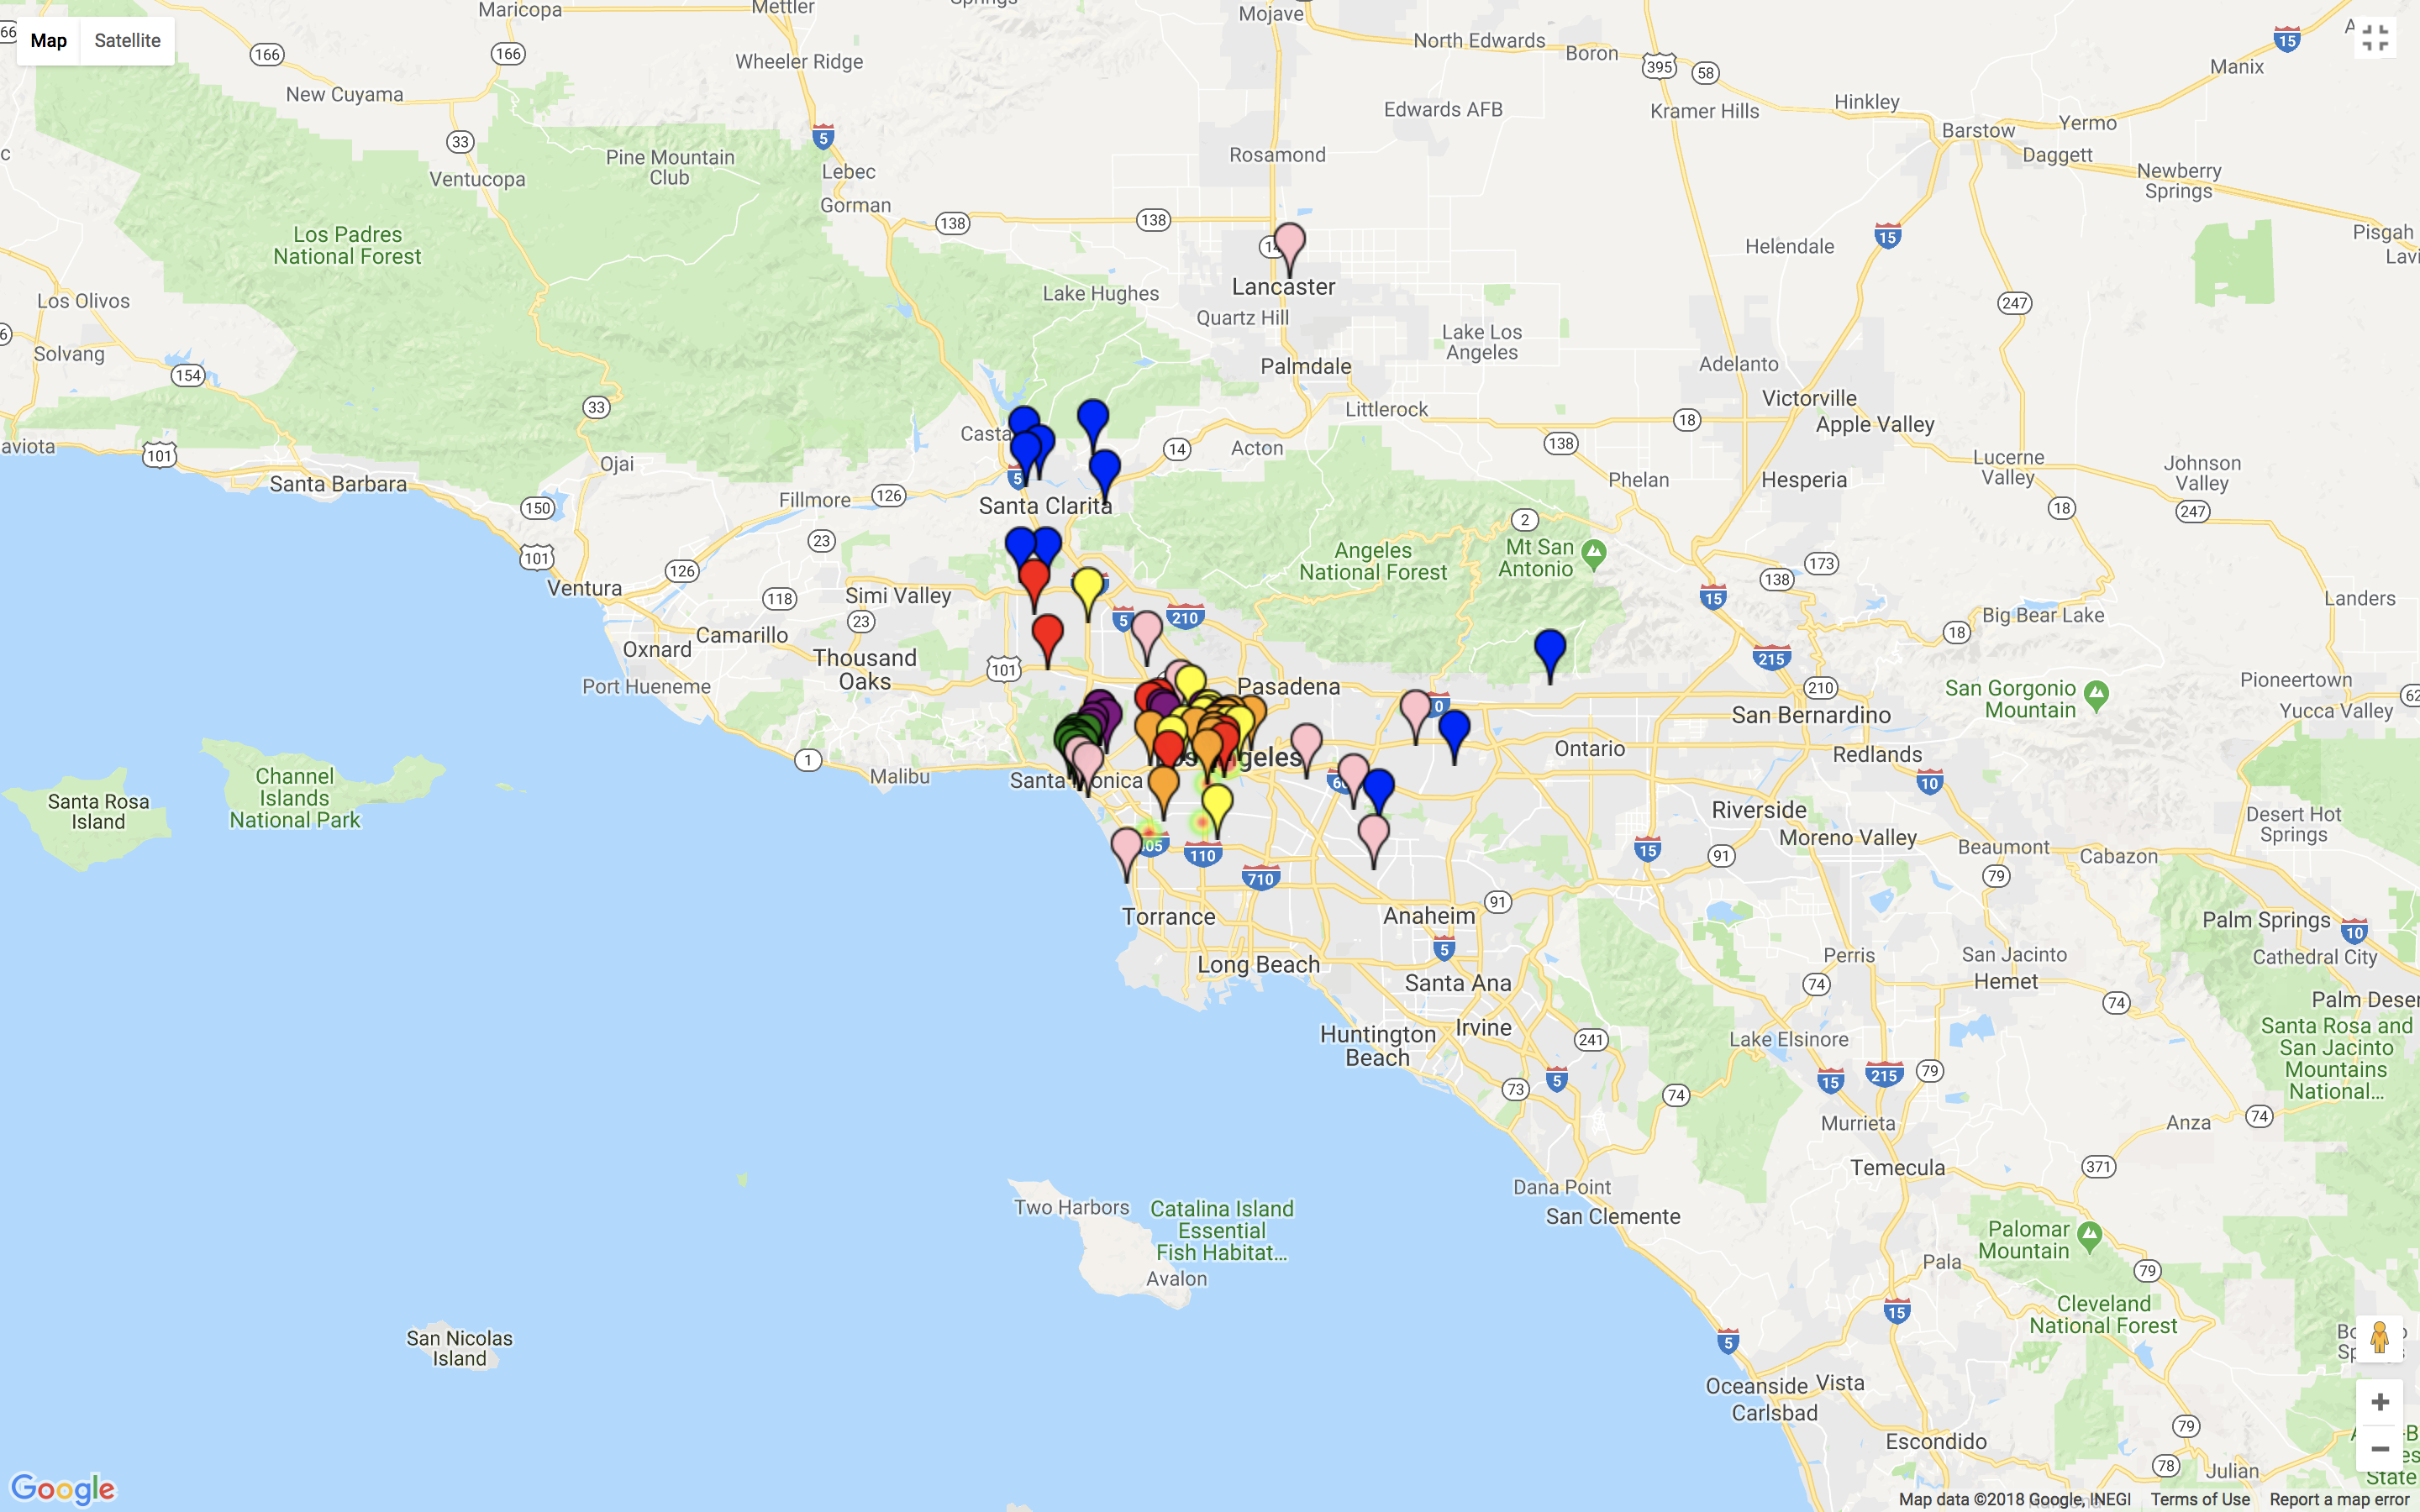
\includegraphics[width=\linewidth]{k=7.png}
  \caption{$k=7$}
\end{figure}

\begin{figure}[H]
  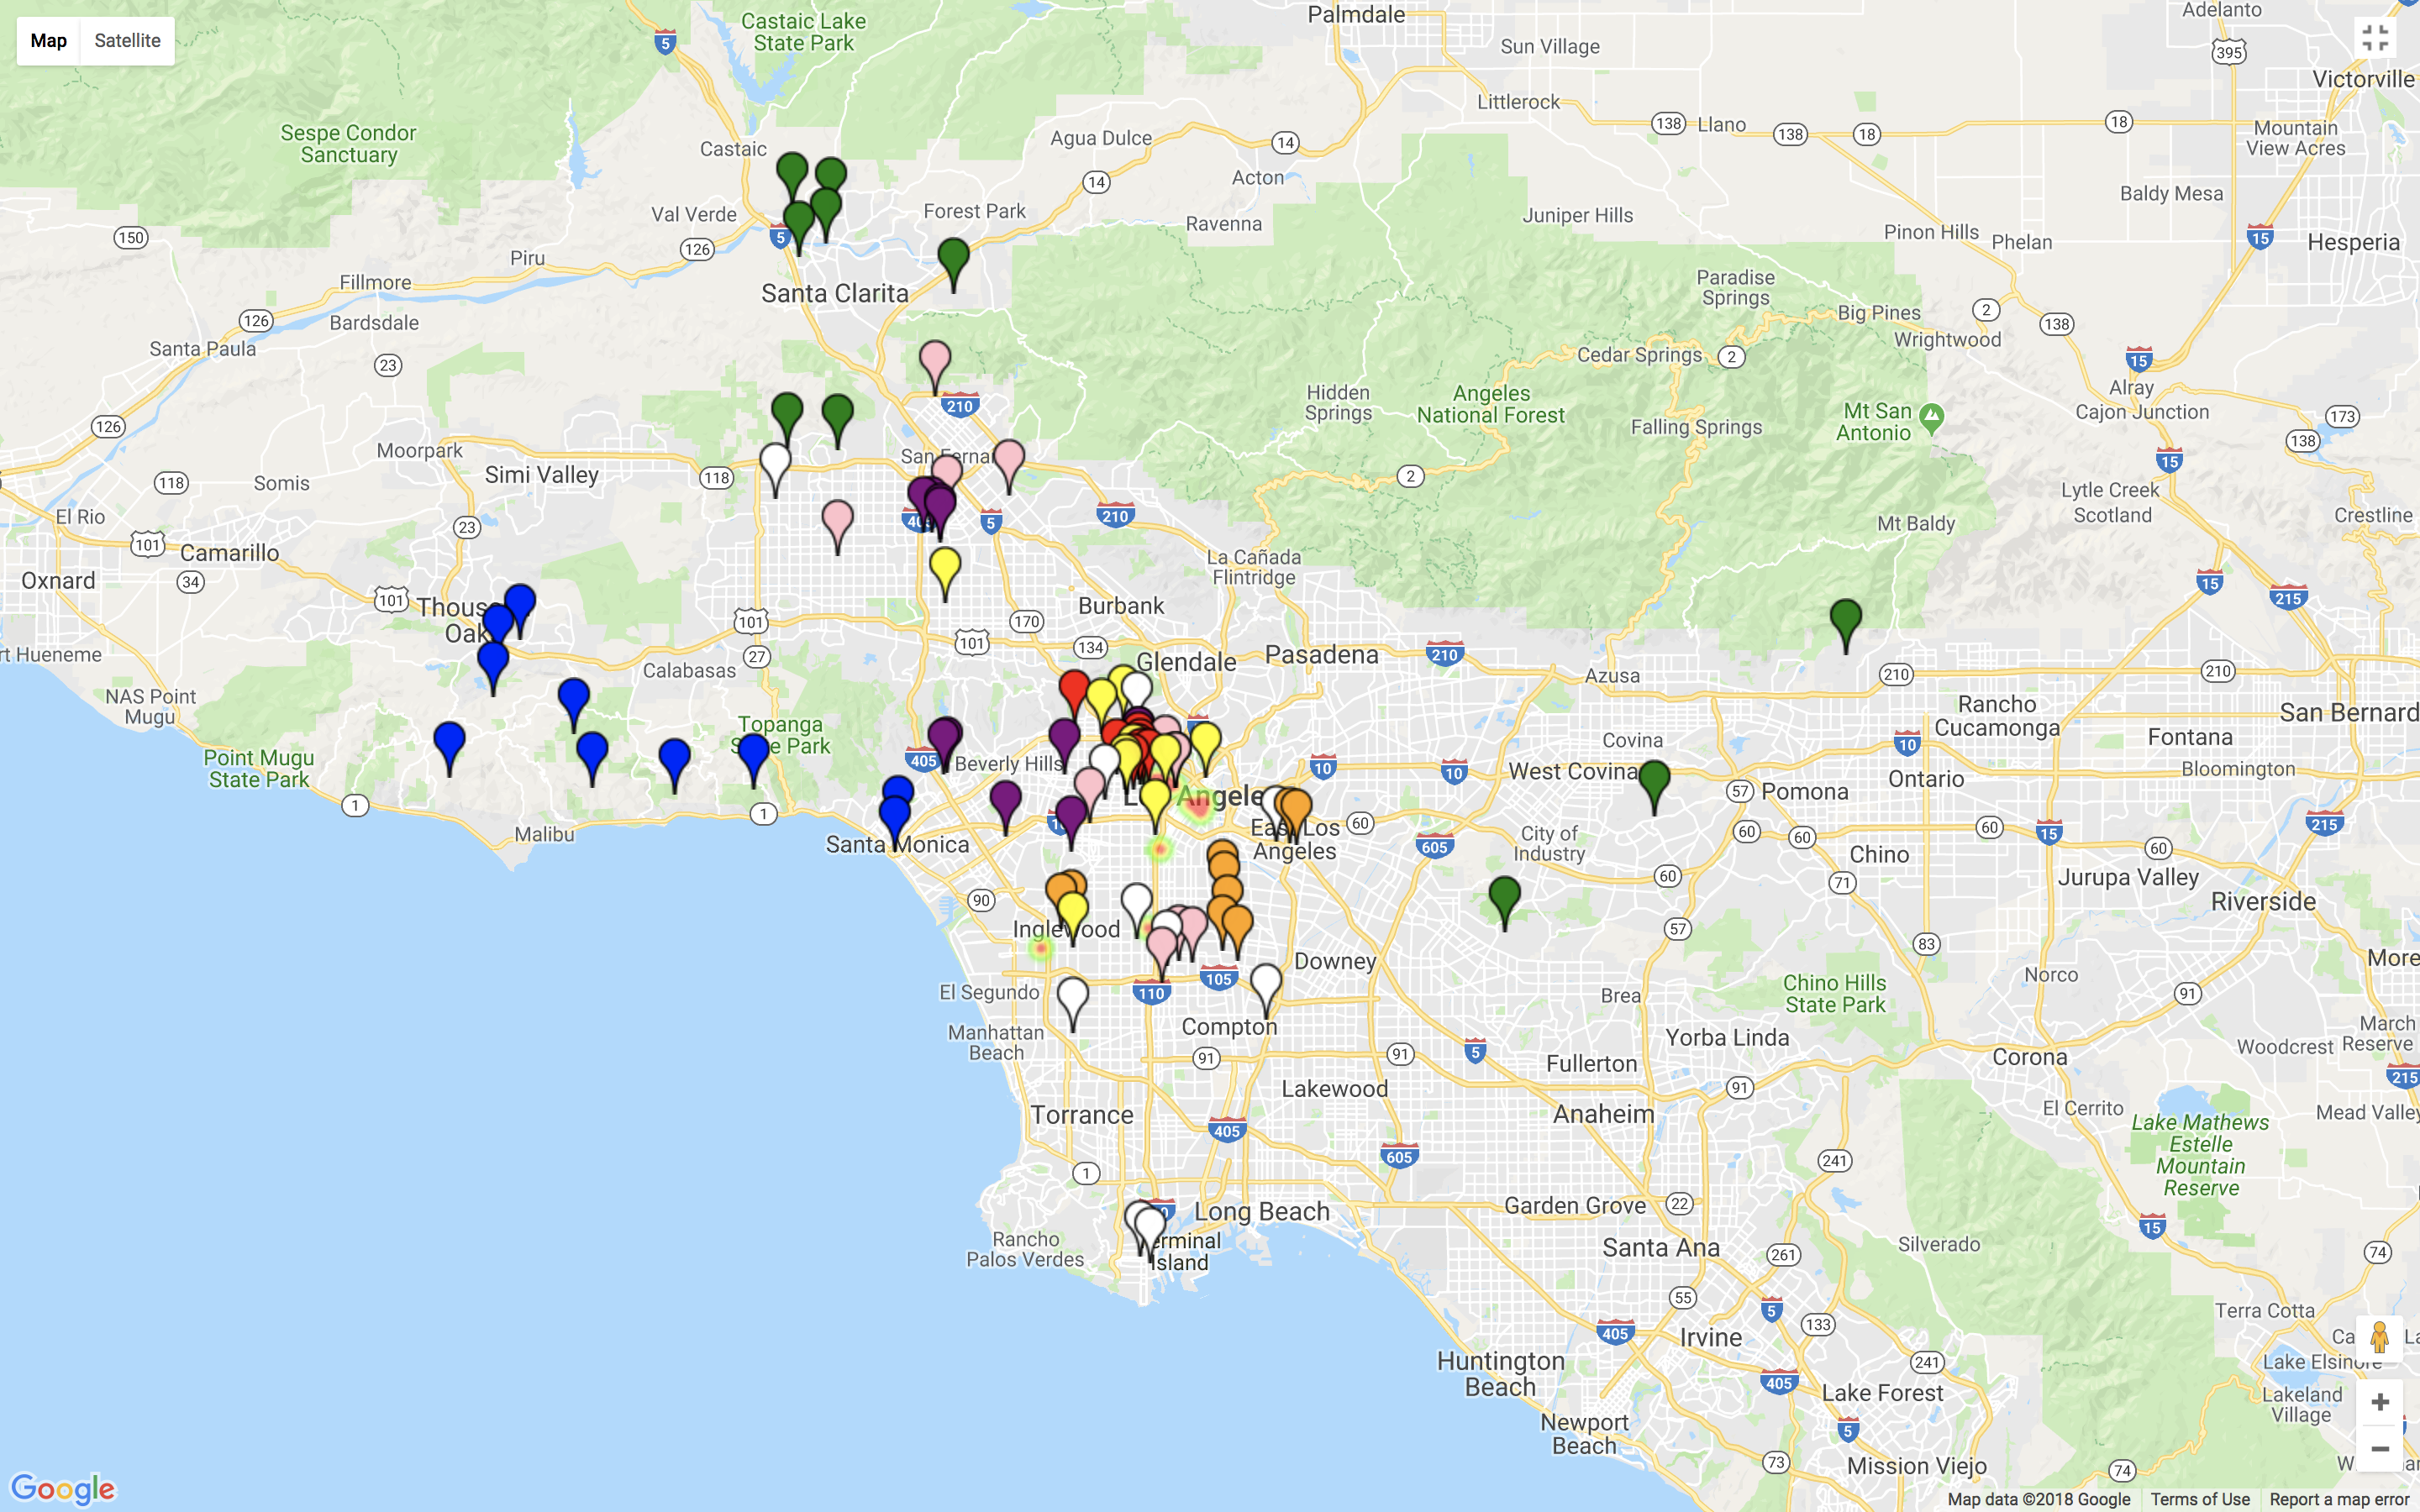
\includegraphics[width=\linewidth]{k=8.png}
  \caption{$k=8$}
\end{figure}
\end{comment}
Moreover, we conducted the non-negative matrix factorization(NMF) to obtain the correlation between the weights of each topic and the homeless population density. For simplicity sake, we will conduct the NMF for number of topics 3 to 5. Denote $\k \in\{2,5\}$ to be the number of topics. From the correlation between the weights of each topic and the homeless population density, for each k, we pick the topic matrix with the highest positive correlation and also pick the topic with highest negative correlation. Below are the matrices with the correlation $\rho$ and the features of topic matrix, i.e coffee shop density and restaurant density.\\

	For \k = 3
\begin{small}
\begin{center}
\begin{tabular}{|c|c|c|c|c|c|c|}
\hline 
$\rho$ & CoffeeDensity & RestaurantDensity & ShelterDensity & CrimeDensity & HousingDensity & BusStopDensity \\ 
\hline 
0.54697  & 0.18935 & 0.40078 & 0.17057          &  0.42859     & 0.2192  & 0.39935    \\ 
\hline 
-0.41816 & 0.23528 & 0.11055 &  0.23629 & 0.083083 &  0.18198 & 0 \\ 
\hline 
\end{tabular} 
\end{center}

\begin{flushleft}
\begin{tabular}{|c|c|c|c|}
\hline 
GenPop2015Density & ZRI & ZHVI & MedHouseholdIncome \\ 
\hline 
0.37516 & 0.35213 & 0.34418 & 0 \\ 
\hline 
0 & 0.39602 & 0.4018 & 0.71993 \\ 
\hline 
\end{tabular} 
\end{flushleft}

\end{small}

	For \k = 4
\begin{small}
\begin{center}
\begin{tabular}{|c|c|c|c|c|c|c|}
\hline 
$\rho$ & CoffeeDensity & RestaurantDensity & ShelterDensity & CrimeDensity & HousingDensity & BusStopDensity \\ 
\hline 
0.61047  & 0 & 0.45189 & 0.2045          &  0.50138     & 0.28931  & 0.39708    \\ 
\hline 
-0.55292 & 0.000158 & 0.17842 & 0.44944 &  0.16865 & 0.44094 &  0\\ 
\hline 
\end{tabular} 
\end{center}

\begin{flushleft}
\begin{tabular}{|c|c|c|c|}
\hline 
GenPop2015Density & ZRI & ZHVI & MedHouseholdIncome \\ 
\hline 
0.36995 & 0.26004 & 0.23822 & 0 \\ 
\hline 
0 & 0 & 0 & 0.73709 \\ 
\hline 
\end{tabular} 
\end{flushleft}
\end{small}

	For \k = 5
\begin{small}
\begin{center}
\begin{tabular}{|c|c|c|c|c|c|c|}
\hline 
$\rho$ & CoffeeDensity & RestaurantDensity & ShelterDensity & CrimeDensity & HousingDensity & BusStopDensity \\ 
\hline 
0.50328  & 0 & 0.56601 & 0.098547 &  0.58106     & 0.20278  & 0.30022    \\ 
\hline 
-0.54216 & 0.26811 & 0.072089 & 0.44805 & 0.027862 &  0.38839 & 0 \\ 
\hline 
\end{tabular} 
\end{center}

\begin{flushleft}
\begin{tabular}{|c|c|c|c|}
\hline 
GenPop2015Density & ZRI & ZHVI & MedHouseholdIncome \\ 
\hline 
0.081367 & 0.32986 & 0.29261 & 0 \\ 
\hline 
0.0077115 & 0 & 0 & 0.73709 \\ 
\hline 
\end{tabular} 
\end{flushleft}
\end{small}

Across the different \k , for the high positive correlation, we can see that the values for the features, RestaurantDensity and CrimeDensity are high. This indicates that census tracks with relatively many restaurants and relatively high crime rates have a high homeless population. Moreover, the MedHouseholdIncome is 0 for all k signifies that the census tracks with low median household income have high homeless population. \\
On the other hand, for the high negative correlations for all \k , the topic matrix exhibits very low values for the BusStopDensity and the GenPop15Density, and a high value for the MedHouseholdIncome. This indicates that the census tracks with low number of bus stops, low general population density and high median household income would have low homeless population. 

From these correlations, we then converted the the census tracks into their respective longitudes and lattitudes using the census tracks as centroids. We plot the heat map graphs to look at the weights of each topic and the homeless population density to compare whether there is overlap of areas of these weights and the homeless population density. Since the weights represents the degree of topic on the census track, The more overlap between the weights and the homeless population density, the more likely that the area has strong presence of homeless population, and thus the more likely that the topic explain the homeless population.

\begin{figure}[H]
  \centering
  	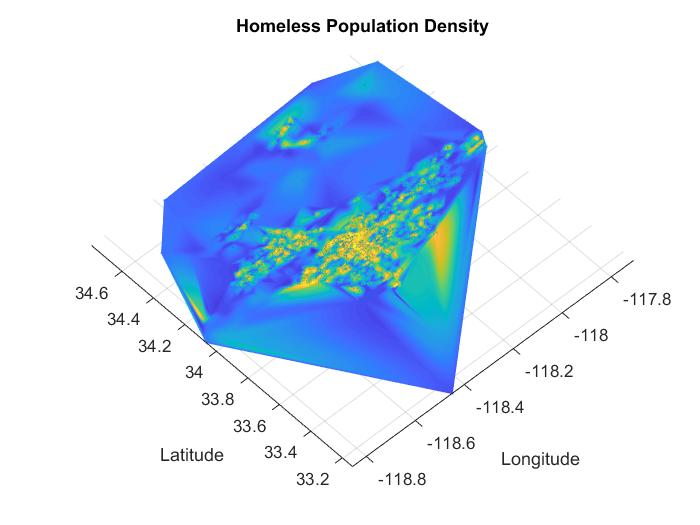
\includegraphics[scale=0.5]{Homeless_pop.jpg}
  	\caption{Homeless Population density}
\end{figure}

\begin{figure}[H]
  \centering
  \subfloat[][Highest Positive Correlation]{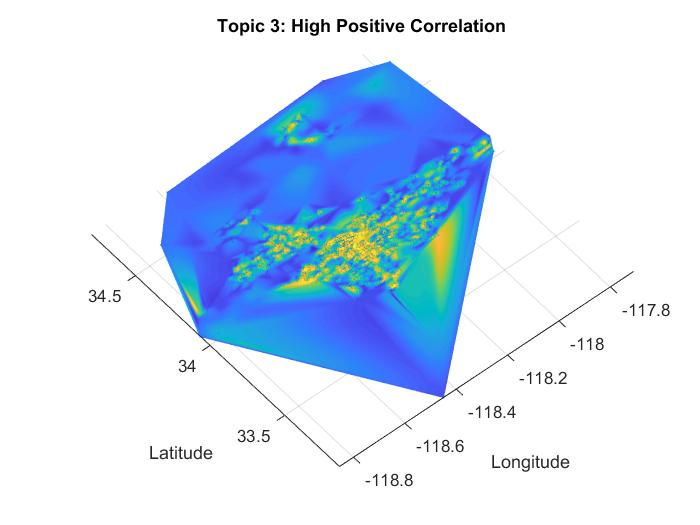
\includegraphics[scale=0.33]{3_topics_H.jpg}
  \label{graph 1}}
  \subfloat[][Highest Negative Correlation]{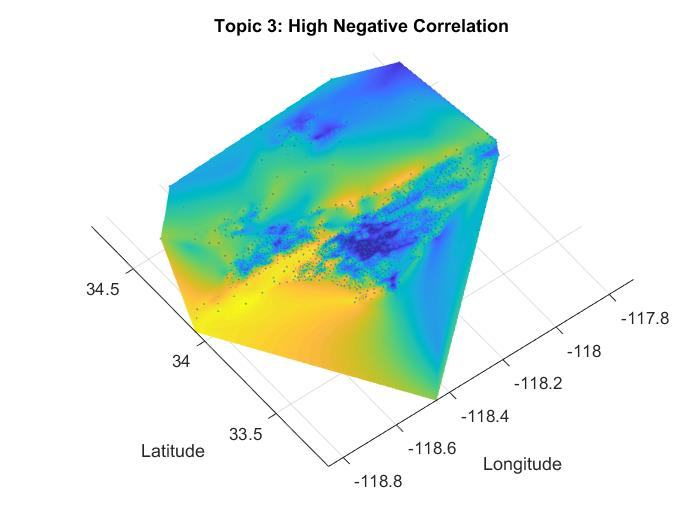
\includegraphics[scale=0.33]{3_topics_L.jpg}
  \label{graph 1}}
  \caption{Number of topics: 3}
\end{figure}

    
\begin{figure}[H]
  \centering
  \subfloat[][Highest Positive Correlation]{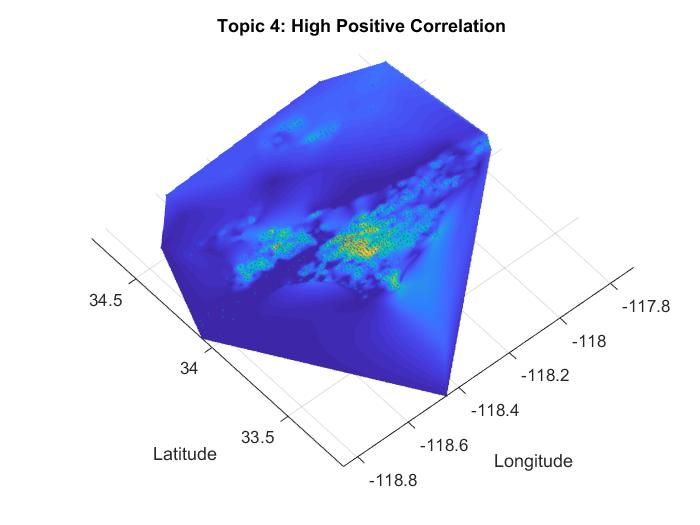
\includegraphics[scale=0.33]{4_topics_H.jpg}
  \label{graph 1}}
  \subfloat[][Highest Negative Correlation]{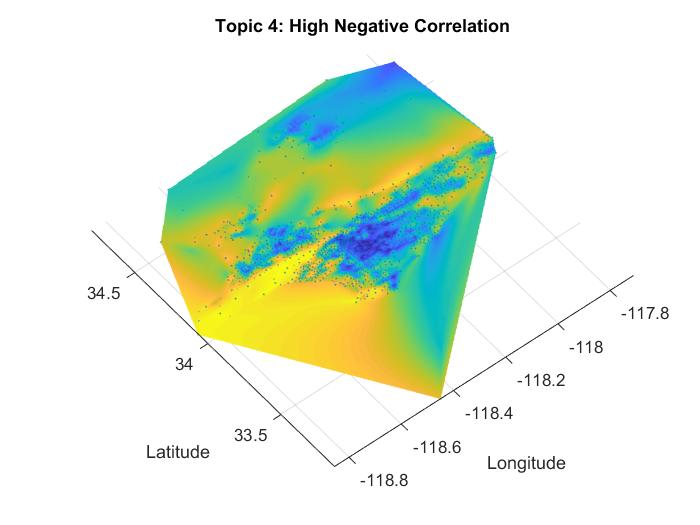
\includegraphics[scale=0.33]{4_topics_L.jpg}
  \label{graph 1}}
  \caption{Number of topics: 4}
\end{figure}


\begin{figure}[H]
  \centering
  \subfloat[][Highest Positive Correlation]{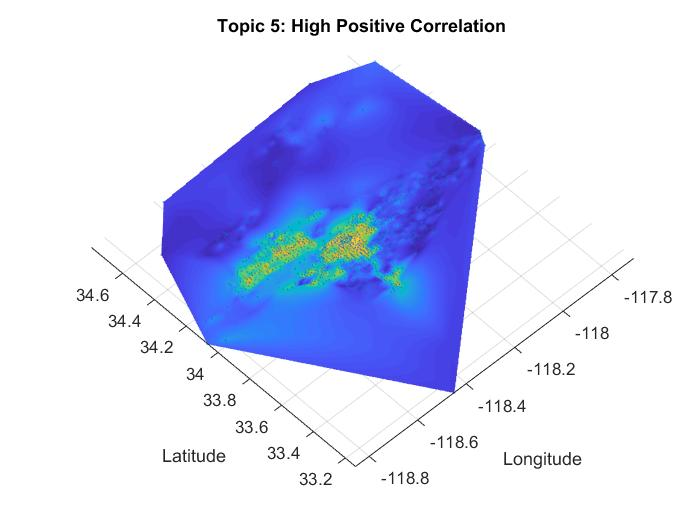
\includegraphics[scale=0.33]{5_topics_H.jpg}
  \label{graph 1}}
  \subfloat[][Highest Negative Correlation]{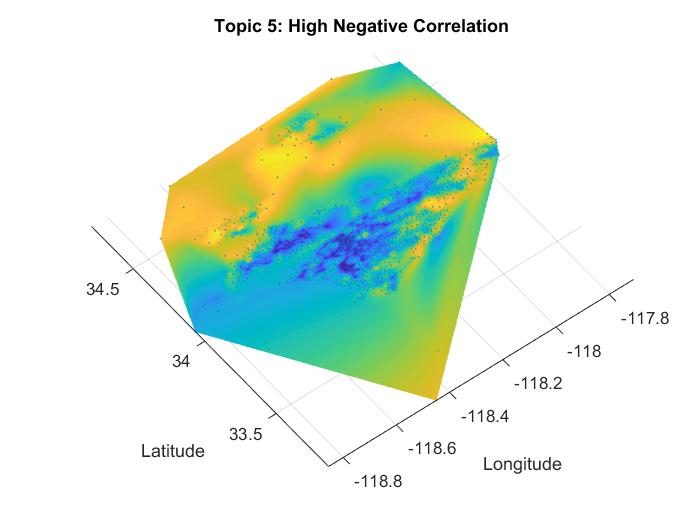
\includegraphics[scale=0.33]{5_topics_L.jpg}
  \label{graph 1}}
  \caption{Number of topics: 5}
\end{figure}

The brighter the map is, the higher the weight/homeless population density. This shows that there is more overlap for topics with the highest positive correlation with the homeless population, while those with the highest negative correlation will have less overlap or close to no overlap, which is consistent to what we would expect. \\

We also compiled the local "variance" of a census track, where (1) The top 10 census tracks with the highest homeless population density,
(2) The top 10 census tracks with the highest local variance, (3) The top 10 census tracks with the lowest local variance.\\


\begin{figure}[H]
\centering
\caption{Table that shows the census tracks with the highest homeless population density, highest local variance and lowest local variance}
\begin{tabular}{|l|l|l|}
\hline
(1)    & (2)    & (3)    \\ \hline
206300 & 207302 & 134101 \\ \hline
209104 & 207301 & 113422 \\ \hline
207301 & 206200 & 119800 \\ \hline
208720 & 206300 & 131300 \\ \hline
208903 & 207502 & 131200 \\ \hline
238320 & 226002 & 109700 \\ \hline
206200 & 211802 & 480101 \\ \hline
208801 & 208904 & 113421 \\ \hline
277400 & 212101 & 111400 \\ \hline
\end{tabular}
\end{figure}

There are many overlaps between the first and the second column, i.e 206300, 207301, etc, which there are none between the first and the third column. This shows that there is clustering of homeless people in the census tracts with the highest variances. This makes sense because we expect that suppose there is large difference in the amenities and the conditions to living within a neighbourhood, there would be more homeless people.

\subsection{Linear Models}

After eliminating predictors that had significant issues of high multicolinearity, and transforming the response variables to achieve constant variance and normally distributed residuals, we identified the statistically significant predictors for explaining variation in each category of a census tracts’ homeless population.

The statistically significant predictors in explaining variation among the homeless population living in vehicles (cars, and campers) are: citations, totcars, mediancome, bus stops, and totencamp people. The Adjusted R-squared for the model explaining variation in vehicle homeless population with street and shelter homeless is  0.434.

\begin{figure}[H]
  \centering
  \caption{Diagnostic Plots for Model Predicting Homeless Population Living in Vehicles}
  
  \begin{subfigures}
  \begin{figure}[H]
    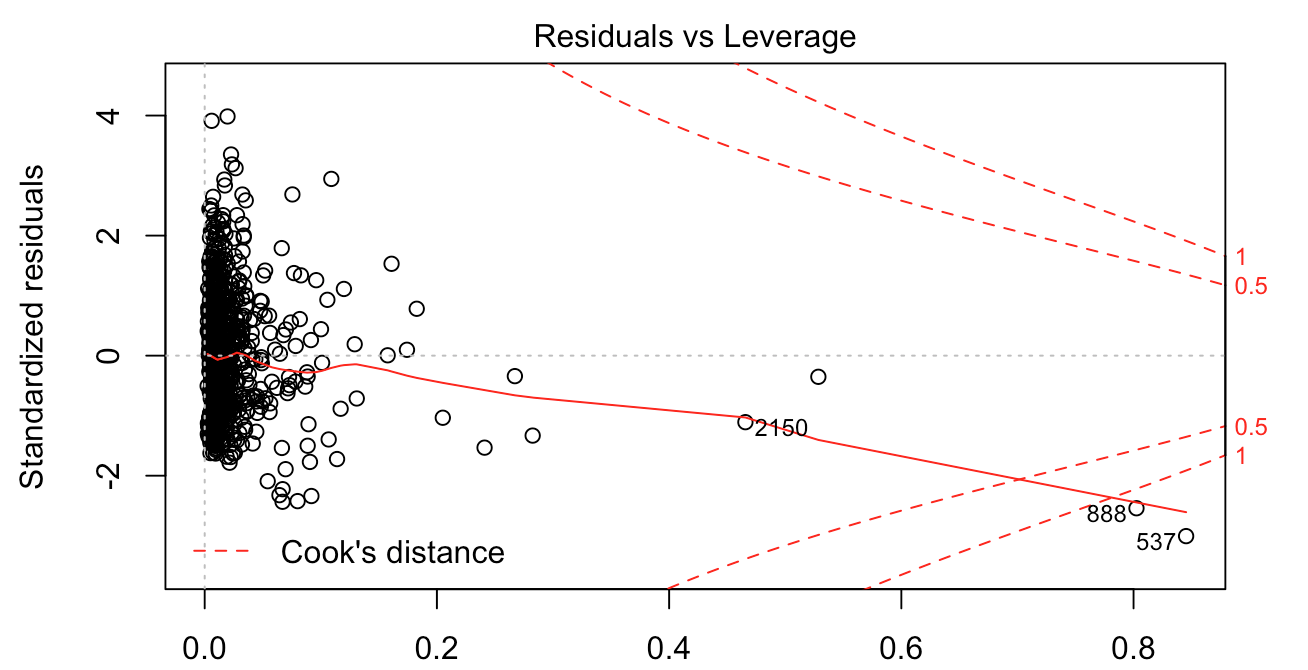
\includegraphics[width=\linewidth, height=0.3\textheight]{carhomeless.png}
  \end{figure}
  %
  \begin{figure}[H]
    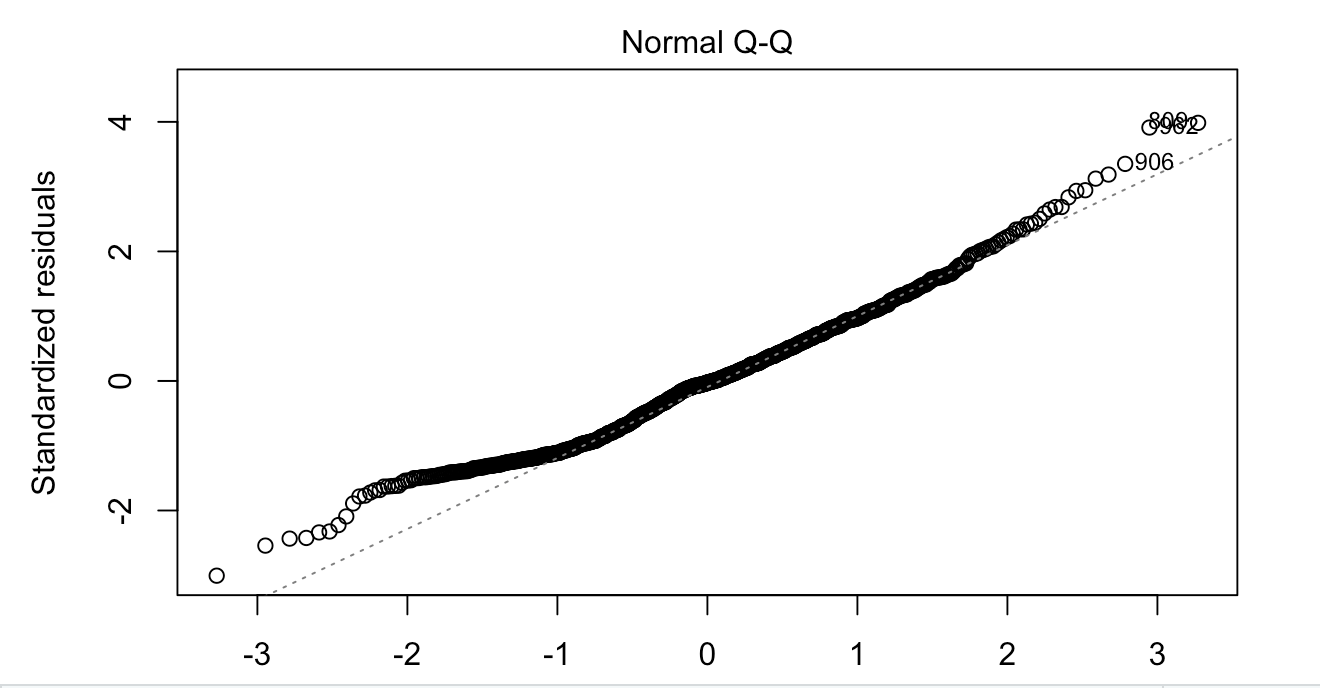
\includegraphics[width=\linewidth, height=0.3\textheight]{carhomeless2.png}
  \end{figure}
  \end{subfigures}

\end{figure}

\begin{figure}[H]\centering
  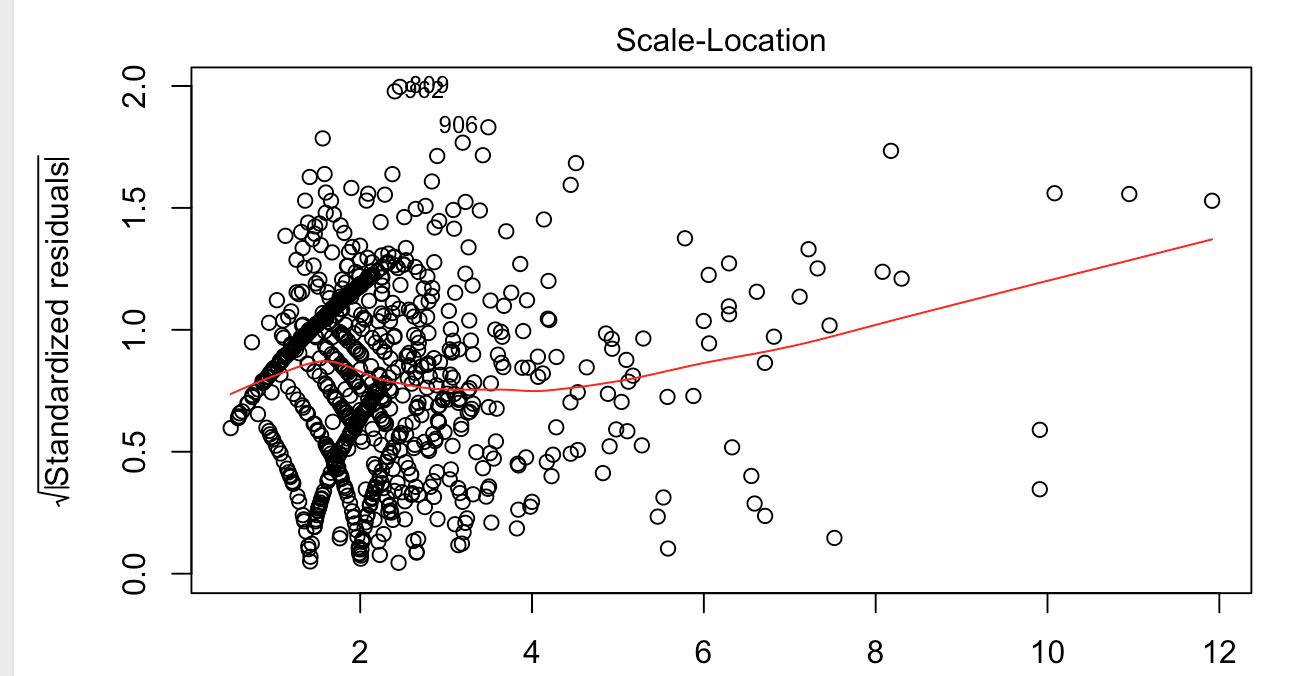
\includegraphics[width=\linewidth, height=0.3\textheight]{carhomeless3.png}
\end{figure}

    From these diagnostic plots, we see that the residuals are normally distributed, and that the residuals are randomly distributed around a mean of zero with constant variance.

Notably, only for predicting the homeless population living in vehicles is the total homeless population count for previous years not a statistically significant predictor. This is likely due to the mobility afforded to the homeless population that live in cars, which makes it so the location of homeless people who live in vehicles is not particularly tied to any certain location.

The model for explaining variation in the shelter homeless population has restaurants, median home income, bus stops, tothomeless2015, tothomeless2016,tottencamp people as its statistically significant predictors.  The adjusted R-squared for this model is 0.8321.


\begin{figure}[H]
\centering
\caption{Modeling Homeless Population Living in Shelters}
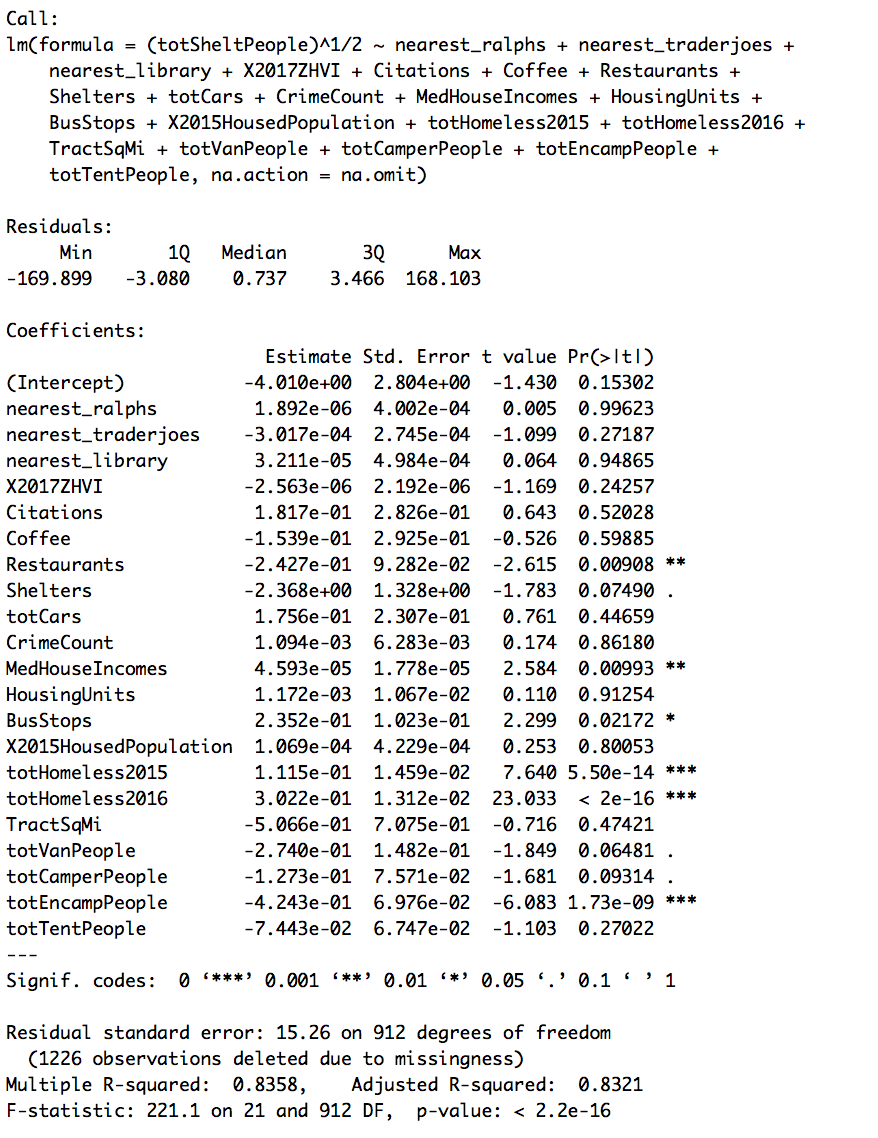
\includegraphics[scale=0.75]{predictingShelterHomeless.png}
\end{figure}

The statistically significant predictors for explaining the variation in a census tracts’ homeless population living on the street in tents and in encampments are the distance to the nearest Trader Joes, distance to the nearest public library, coffee shops, crime count, affordable housing units, bus stops, the 2015 total homeless population the 2016 total homeless population, total number of vans, and the total number of shelter. This model’s Adjusted R-squared is 0.7536.

\begin{figure}[H]
\centering
\caption{Modeling Homeless Population in Tents and Encampments}
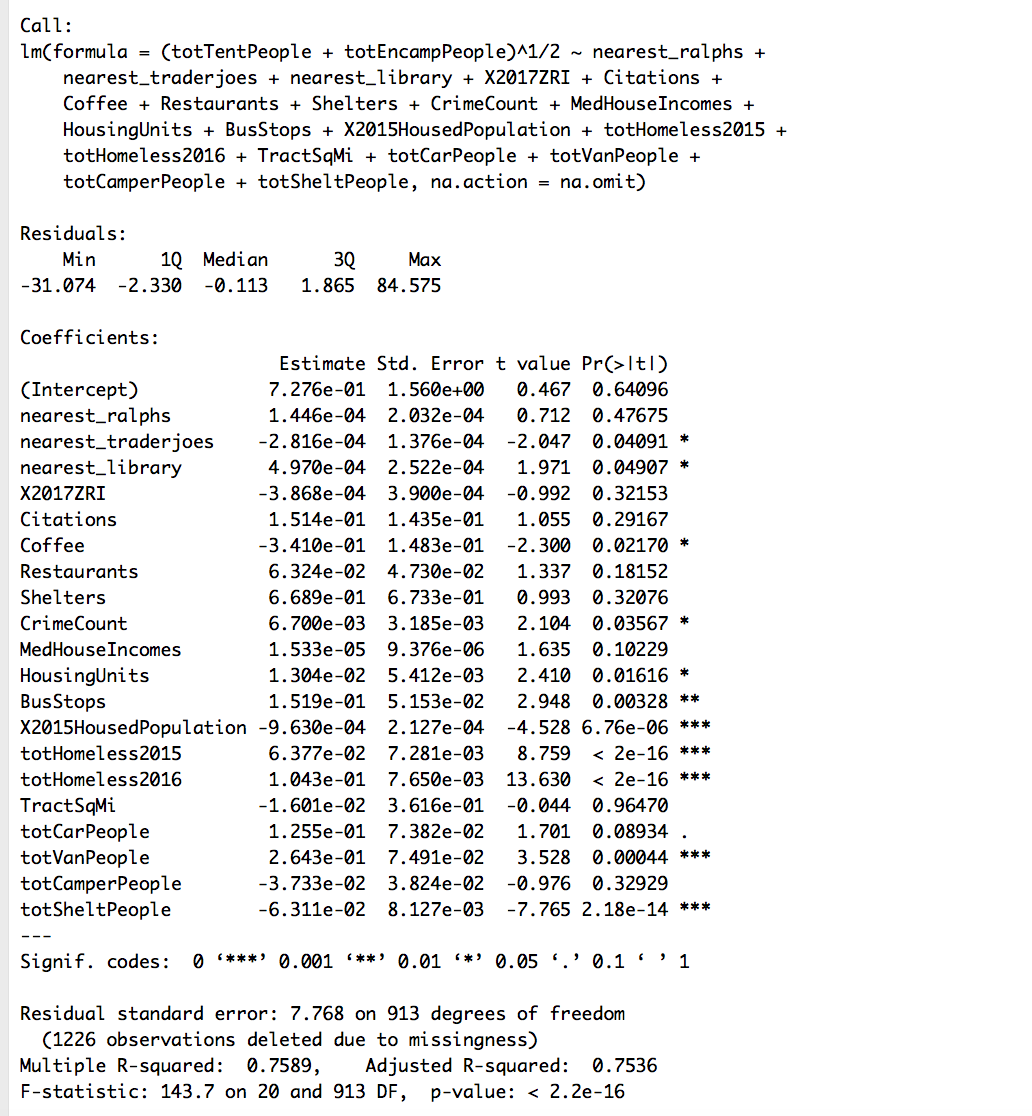
\includegraphics[scale=0.75]{predictingStreetHomeless.png}
\end{figure}

Next, we reconstructed models for the three homeless populations using a forward stepwise regression process. In each step, this stepwise regression process will consider a variable for addition from the set of explanatory variables based on some prespecified criterion. We constructed models using both AIC and BIC as criterions.

The selected predictors for modeling the homeless population living in shelters when using BIC as the criterion for inclusion are  totCars, totEncampPeople, MedHouseIncomes, BusStops, and Coffee. The adjusted R-squared for the forward stepwise regression model created using BIC as a criterion is 0.4337.
 
When using AIC to select predictors for the homeless population living in shelters, the Adjusted R-squared only slightly increased to  0.4348, and the number of predictors selected increased to include totCamperPeople, totVanPeople,  totCarPeople,  totCars , MedHouseIncomes,  X2015HousedPopulation , nearest\_library,  Bus Stops,  Coffee , nearest\_traderjoes , X2015ZRI, and X2017ZRI. This is due to AICs tendency to overfit because of its smaller penalty for increasing the number of predictors.

The selected predictors for modeling the homeless population living on the street using AIC as a criterion are totHomeless2016, totVanPeople, CrimeCount, X2015HousedPopulation, BusStops, HousingUnits,  totSheltPeople , totHomeless2015 , nearest\_library,  coffee , nearest\_traderjoes, and totCars.
 
The selected predictors for explaining the variation in the homeless population living on the street using forward stepwise regression with BIC as the criterion are totHomeless2016, totVanPeople,  CrimeCount , X2015HousedPopulation , BusStops, HousingUnits. Again, we see that models constructed using BIC include fewer predictors because of BICs greater penalty for increasing the number of predictors. 

\begin{figure}[H]
\centering
\caption{Visualizing Size of Homeless Populations With The Brand of Nearest Grocery Store}
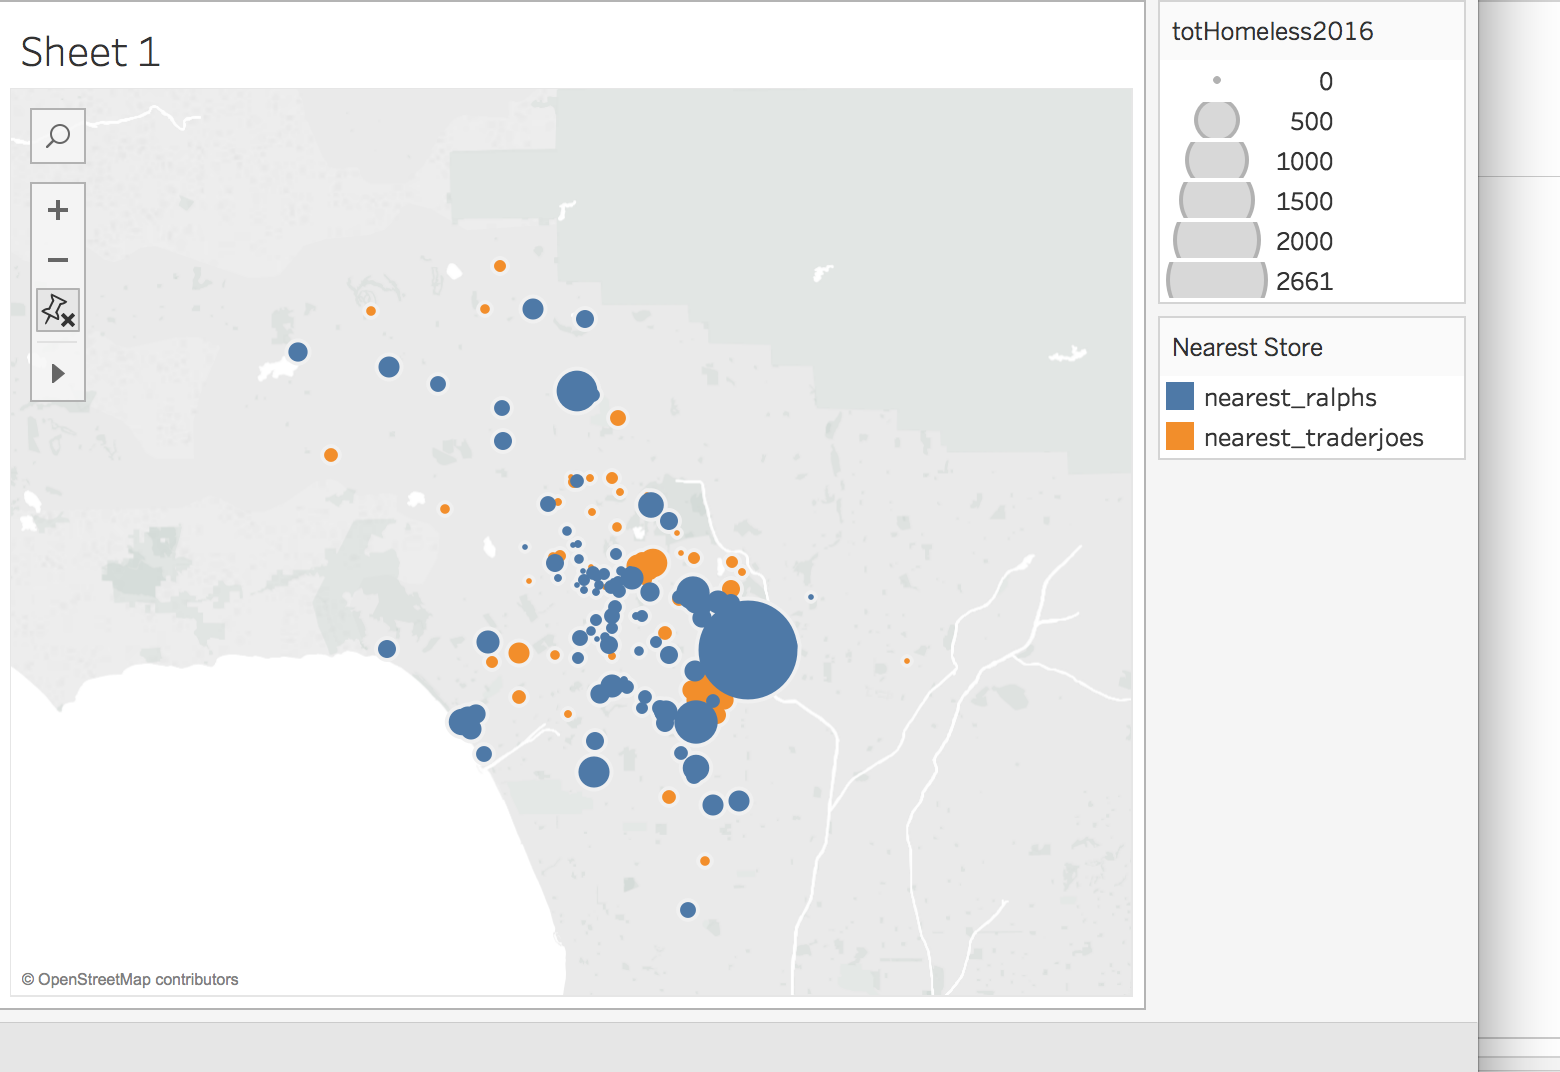
\includegraphics[scale=.5]{plot_homless_with_nearestStore.png}
\end{figure}

It appears that census tracts with larger homeless populations tend to be in closer proximity to Ralphs, while census tracts with smaller homeless populations tend to be in closer proximity to Trader Joes.

\begin{figure}[H]
\centering
\caption{Visualizing Size of Homeless Populations With Proximity to Public Libraries}
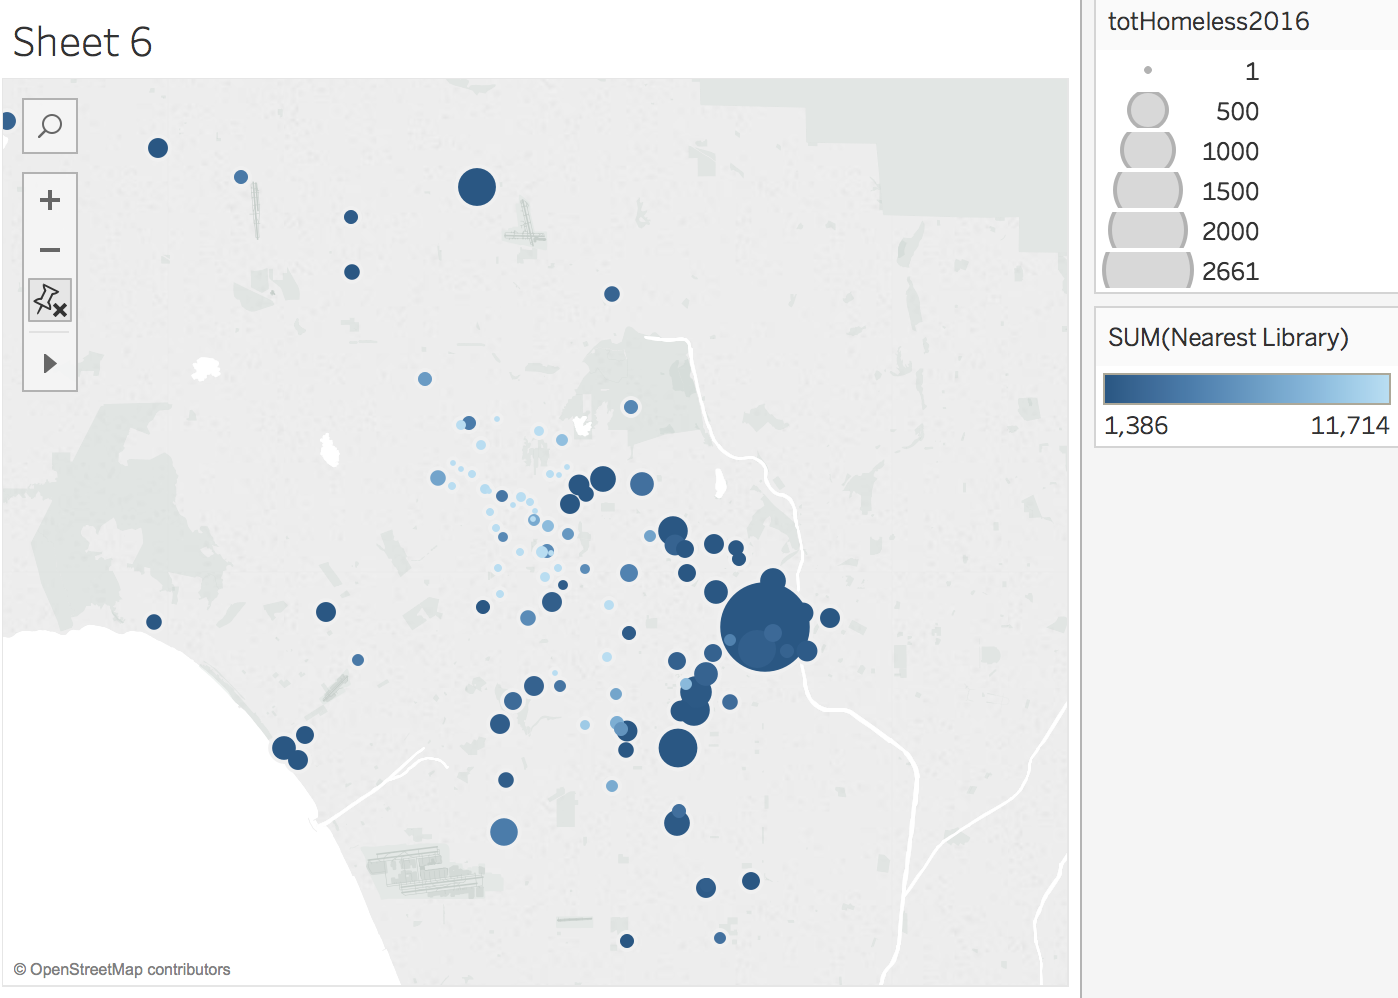
\includegraphics[scale=.5]{dark_libs.png}
\end{figure}

It appears that census tracts with larger homeless populations tend to be in closer proximity to Public Libraries, while census tracts that are farther from Public Libraries tend to have smaller homeless populations.

\subsection{Neural Networks}

Because of the uneven distribution of the bins, we use different measurement to reflex how well the algorithm do. Apart from the accuracy, we have confusion matrix and precision. Accuracy can be calculated by:
\begin{align}
A = \frac{\text{\# of correct predictions}}{\text{\# of all predictions}}
\end{align}
A confusion matrix $C$ is a table that is often used to describe the performance of a classification model on a set of test data for which the true values are known. The $(i,j)$ entry of the matrix represents  the number of point whose true value is the $i^{th}$ class and it was predicted to the $j^{th}$ class. Precision$i$ is the ratio of true predictions among all the points that was predicted to be in the $i^{th}$ class:
\begin{align}
\text{Precision i} = \frac{C[i,i]}{\sum_j C[i,j]}
\end{align}

The table below shows the best result of the ternary classification for bucket division: [-400,-20), [-20,20), [20,600).\\

\begin{tabular}{c||ccccccc}
\hline 
Model & Preprocessing & Accuracy & Training Cost & Testing Cost & Hidden & Output \\ 
\hline 
A & PCA & 0.725 & 0.359 & 0.501 & - & Sigmoid \\ 
\hline 
\end{tabular} \\\\
With a confusion matrix and precision:\\
\begin{center}
\begin{tabular}{c|ccc}
- & True 0 & True 1 & True 2 \\ 
\hline 
Pred 0 & 4 & 19 & 2 \\ 
Pred 1 & 46 & 346 & 61 \\ 
Pred 2 & 2 & 4 & 3 \\ 
\end{tabular}
\end{center} 
\ \\
\begin{center}
\begin{tabular}{ccc}
\hline 
Precision0 & Precision1 & Precision2 \\ 
\hline 
0.160 &  0.764 & 0.333 \\ 
\hline 
\end{tabular}
\end{center}
\ \\

We need to take more care when we look at the precision numbers. Because of the imbalance of the numbers of data points in each bin, if we have a purely chance predictor, the precision will be the ratio of the number of data point in that bin to the number of data point in total. Thus a pure chance model will have a precision:\\
\begin{center}
\begin{tabular}{ccc}
\hline 
Precision0 & Precision1 & Precision2 \\ 
\hline 
0.070 &  0.758 & 0.136 \\ 
\hline 
\end{tabular}
\end{center}
Thus even though the precision number looks bad, all of them in fact are bigger than the change model. Therefore our model is performing better than chance at predicting change in homeless population. 

We change the cutoff point so that the three bins to have roughly equal amount. The table below shows the best result of the ternary classification for bucket division: [-400,-3), [-3,6), [6,600).\\

\begin{tabular}{c||ccccccc}
\hline 
Model & Preprocessing & Accuracy & Training Cost & Testing Cost & Hidden & Output \\ 
\hline 
B & Normalization & 0.389 & 0.397 & 0.914 & relu & Sigmoid \\ 
\hline 
\end{tabular} \\\\
With a confusion matrix and precision:\\
\begin{center}
\begin{tabular}{c|ccc}
- & True 0 & True 1 & True 2 \\ 
\hline 
Pred 0 & 60 & 49 & 60 \\ 
Pred 1 & 58 & 79 & 48 \\ 
Pred 2 & 48 & 35 & 51 \\ 
\end{tabular}
\end{center} 
\ \\
\begin{center}
\begin{tabular}{ccc}
\hline 
Precision0 & Precision1 & Precision2 \\ 
\hline 
0.355 & 0.427 &  0.380 \\ 
\hline 
\end{tabular}
\end{center}
\ \\

A pure chance model for this one would result in a precision of:\\
\begin{center}
\begin{tabular}{ccc}
\hline 
Precision0 & Precision1 & Precision2 \\ 
\hline 
0.333 & 0.333 &  0.333 \\ 
\hline 
\end{tabular}
\end{center}
\ \\
The precision of our model is higher than each of it's corresponding entry in the chance model. Therefore our model performs better than chance.

\section{Summary and Future Work}
\subsection{Earth Mover's Distance}
Further geospatial analysis is to come with the topic modelling plots using the earth mover’s distance (EMD), or the Wassertein metric. The earth mover’s distance describes the cost of moving from one geospatial cluster to the a new geospatial cluster. In our applications this can be used to determine the cost of moving to one census tract to the next or from one cluster of topic model to another.

Take a cluster of points denoted \textbf{P} such that $\textbf{P} = \lbrace (p_{1}, w_{p1}), ..., (p_{i}, w_{pi})   \rbrace$ where $p_{i}$ is the cluster representative and $w_{pi}$ is the weight of clusters. Similarly, take another cluster of points denoted \textbf{P} such that $\textbf{Q} = \lbrace (p_{1}, w_{q1}), ..., (q_{j}, w_{qj})   \rbrace$. Take $\textbf{D} = [d_{ij}]$ to be the ground clusters between clusters $p_{i}$ and $q_{j}$

Our goal is to find flow $ \textbf{F}=[f_{ij}]$ with $f_{i,j}$ being the flow between $p_{i}$ and $q_{j}$ that minimizes the overall cost. This can be done by solving the optimization function:$$min \sum_{i=1}^{m} \sum_{j=1}^{n} f_{i,j}d_{i,j}$$

\subsection{Neural Network Exploration}
Future research should explore more method of prepossessing the data. Considering the error in public database, we could put the feature data into bins as well (e.g.: income can be slit into 5 bins according to it's standard deviation). 

\subsection{Convolutional Neural Network}
Convolutional neural network is also promising in the context of analyzing the change in homeless population because homeless population move around frequently. Change in one area will change the number of homeless population in other areas. 

\section{Acknowledgments}

We thank our adviser and mentor, Professor Michael Lindstrom, for all of his advice and help on this project.

\newpage

\printbibliography
\end{document}

